\documentclass[times, utf8, diplomski]{fer}
\usepackage{booktabs}
\usepackage{color}
\usepackage{listings}
\usepackage{pdfpages}
\usepackage{subcaption}
\usepackage{float}

\graphicspath{ {./resources/images/} }
\renewcommand{\lstlistingname}{K\^{o}d}%
\lstset{ %
language=C++,                % choose the language of the code
basicstyle=\footnotesize,       % the size of the fonts that are used for the code
numbers=left,                   % where to put the line-numbers
numberstyle=\footnotesize,      % the size of the fonts that are used for the line-numbers
stepnumber=1,                   % the step between two line-numbers. If it is 1 each line will be numbered
numbersep=5pt,                  % how far the line-numbers are from the code
backgroundcolor=\color{white},  % choose the background color. You must add \usepackage{color}
showspaces=false,               % show spaces adding particular underscores
showstringspaces=false,         % underline spaces within strings
showtabs=false,                 % show tabs within strings adding particular underscores
frame=single,           % adds a frame around the code
tabsize=2,          % sets default tabsize to 2 spaces
captionpos=b,           % sets the caption-position to bottom
breaklines=true,        % sets automatic line breaking
breakatwhitespace=false,    % sets if automatic breaks should only happen at whitespace
escapeinside={\%*}{*)}          % if you want to add a comment within your code
}

\begin{document}

% TODO: Navedite broj rada.
\thesisnumber{2926}

% TODO: Navedite naslov rada.
\title{3D interaktivna vizualizacija simulacije vibracija}

\author{Nikola Vugdelija}

\maketitle

% Ispis stranice s napomenom o umetanju izvornika rada.
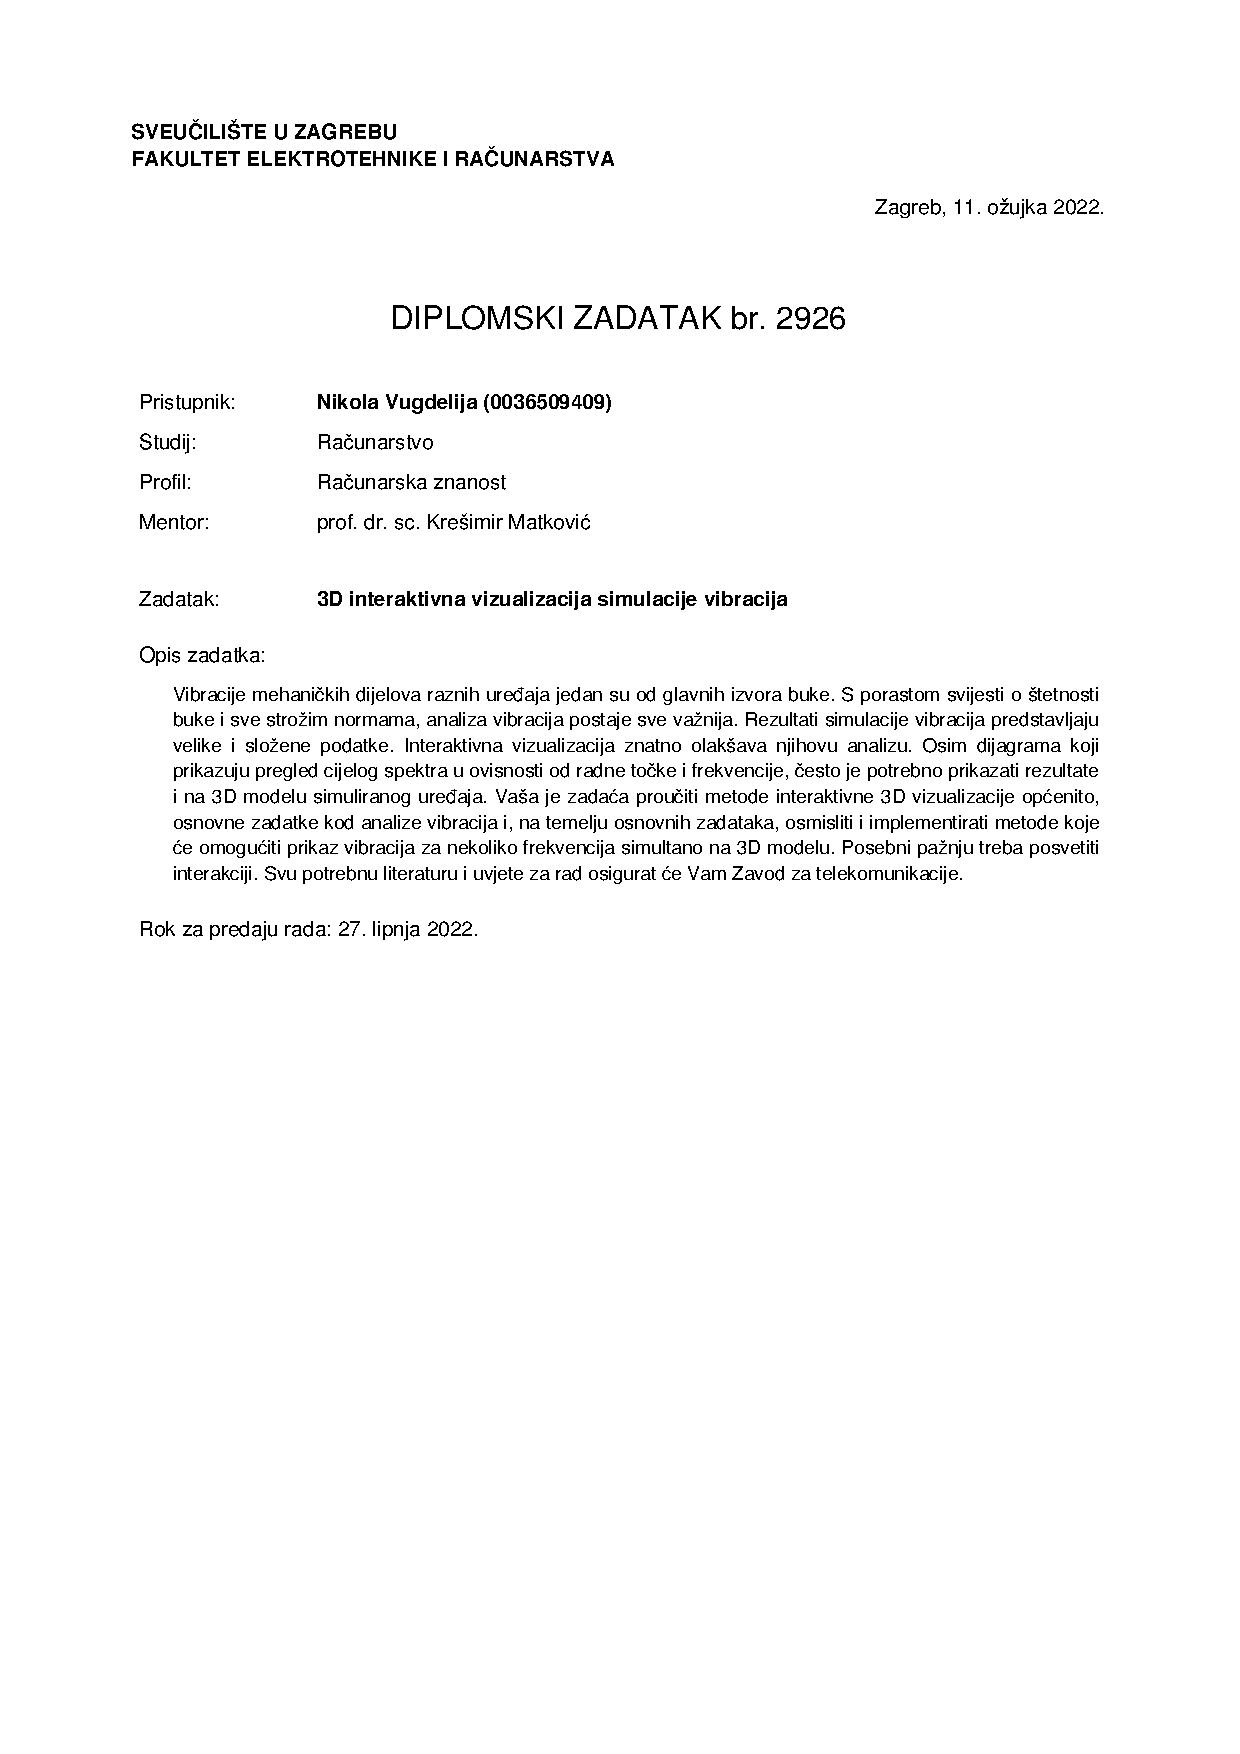
\includepdf[pages=-]{resources/docs/task.pdf}


% Dodavanje zahvale ili prazne stranice. Ako ne želite dodati zahvalu, naredbu ostavite radi prazne stranice.
\zahvala{Zahvala će biti ovdje kad je formuliram u glavi.}

\tableofcontents

\listoffigures

\chapter{Uvod}
Buka i vibriranje motora su jedni od ključnih faktora koji utječu na osjećaj udobnosti putnika u osobnom automobilu. No, iako se može reći kako je osjećaj udobnosti subjektivne prirode, propisi koji kontroliraju dozvoljene razine buke koju u okolišu proizvodi motor vozila su objektivni i egzaktni. Zbog navedenih razloga je inženjerima iznimno važno održati vibriranje motora na što nižoj razini prilikom rada, a najjednostavniji način na koji to mogu provjeriti u fazi projektiranja motora je pomoću NVH \engl{Noise, Vibration, Harshness} simulacija. NVH simulacije inženjerima omogućuju precizan uvid u razinu vibriranja pojedinih dijelova motora, a probleme koji mogu uzrokovati vibraciju mogu rješavati prilikom projektiranja.\\

No, računanje simulacije je samo dio problema. U radu \citep{matkovic2021getting} je naglašeno kako računske simulacije ove vrste, nerijetko proizvode podatke koje se ne može jednostavno vizualizirati i analizirati. Stoga je potrebno podatke prikazati intuitivno i razumljivo kako bi ih stručnjaci mogli koristiti na što efikasniji način. Iako su podaci prikazani u obliku tablica i grafova korisni, vizualizacijom istih podataka na 3D modelu motora se postiže jasniji, intuitivniji i potpuniji prikaz potencijalnih izvora buke.\\

Ovaj rad opisuje izradu alata za vizualizaciju podataka dobivenih iz NVH simulacije pomoću 3D modela motora i 2D grafova. Fokus predstavljenog alata je na vizualizaciji snage vibracije dijelova motora s obzirom na višestruke frekvencije vibriranja motora, kako bi se razine vibracije različitih taktova motora jednostavnije uspoređivale.

\chapter{Pregled područja}
Vizualizacija podataka je iznimno važno područje analize podataka. Budući da isti skup podataka može prenijeti potpuno drugačije informacije ovisno o načinu prikaza, od velike je važnosti odabrati optimalne vizualizacijske tehnike za konkretni skup podataka. Kako je naglašeno u članku \citep{Unwin2020Why}, kod vizualizacije ne postoji jedna, "optimalna" grafika koja vrijedi za svaki skup podataka, nego je često potrebno pronaći grupu vizualizacijskih tehnika koje se međusobno upotpunjuju i prikazuju cjelovitu sliku. Stoga je tijekom osmišljavanja alata za vizualizaciju izrazito važno utvrditi za koju svrhu se taj alat koristi, te koje informacije je potrebno njime vizualizirati iz danog skupa podataka. Odgovori na navedena pitanja postaju kompleksniji za odgonetnuti s porastom kompleksnosti skupa podataka koji alat vizualizira. Zbog toga je pomoć stručnjaka u domeni itekako korisna.\\

Kao što je već spomenuto, glavna svrha alata razvijenog u sklopu ovog rada je vizualizacija NVH podataka na modelu motora. Prilikom izrade ovog rada je korišten isti skup podataka koji je korišten prilikom izrade alata u sklopu rada \citep{matkovic2021getting}. Spomenuti podaci su izračunati NVH simulacijom pomoću alata AVL EXCITE™ \citep{avlEXCITE}. Motor je zadan kao skup ćelija, a za svaku ćeliju su poznate koordinate okolnih točaka u 3D prostoru, te kojom snagom ćelija vibrira pri različitim frekvencijama vibracije motora.\\

Kako je spomenuto u radu \citep{matkovic2021getting}, stručnjake pri analizi NVH podataka ponajprije zanimaju tri stavke:

\begin{itemize}
\item Usporedba snage vibriranja motora na različitim frekvencijama vibracije motora
	\begin{itemize}
	\item Kako se snaga vibracije mijenja na pojedinim dijelovima motora s promjenom frekvencije vibracije motora?
	\end{itemize} 
\item Lokalizacija značajki
	\begin{itemize}
	\item Koje ćelije motora pri zadanoj frekvenciji vibriraju snagom koja pripada zadanom rasponu?
	\end{itemize} 
\item Lokalna pretraga
	\begin{itemize}
	\item Kojom snagom vibriraju odabrane ćelije?\\
	\end{itemize} 
\end{itemize}

Alat razvijen u sklopu rada \citep{matkovic2021getting} dobro adresira navedene značajke. Koristeći paralelne koordinate, omogućen je detaljan pregled usporedbe podataka na različitim frekvencijama vibracije motora. Adresiranje druge i treće značajke je olakšano omogućavanjem korištenja višestrukih, međusobno povezanih prozora s 3D prikazom motora. Lokalna pretraga je ostvarena uz pomoć interaktivne selekcije koju korisnik može koristiti za biranje raspona snage vibracije za određene frekvencije, a svi prozori automatski ažuriraju prikaz modela motora označujući ćelije koje pripadaju zadanim rasponima. Konačno, u radu \citep{matkovic2021getting} je lokalna pretraga omogućena bojanjem modela motora bazirano na snazi vibracije pojedinačnih ćelija pri zadanoj frekvenciji vibriranja motora. Detaljniji uvid u snagu vibriranja pojedine ćelije modela je omogućen odabirom interesne ćelije, nakon čega se istakne 2D graf vibracija  zadane ćelije.\\

No, iako je referirani rad cjelokupno odlično pokrio sve tri značajke, u području usporedbe snage vibracije dijelova motora na različitim frekvencijama vibracije još ima prostora za napredak. Naime, trenutna usporedba podataka na različitim frekvencijama je moguća samo pomoću 2D grafova, koji iako korisni, imaju problema s čitljivošću i jasnoćom. Alat koji je razvijen u sklopu ovog rada implementira niz vizualizacijskih tehnika koje potencijalno povećavaju intuitivnost usporedbe vibracija dijelova motora na različitim frekvencijama vibriranja u odnosu na izvedbu kod alata razvijenog u radu \citep{matkovic2021getting}.

\chapter{Analiza zadatka i zahtjeva}
Budući da dizajniranje alata za vizualizaciju nije jednostavan zadatak, potrebno je poduzeti određene predprodukcijske korake kako bi se osigurala zadovoljavajuća implementacija glavnog zadatka. Navedeni je zadatak potrebno dodatno analizirati, čime bi se uočili zahtjevi potrebni za njegovo uspješno odrađivanje. Identificirane zahtjeve je također potrebno analizirati, kako bi se utvrdila njihova povezanost s glavnim zadatkom, te osiguralo njihovo uspješno i cjelovito zadovoljavanje. 

\section{Identificirani zadaci}
Ključni zadatak alata razvijenog u sklopu ovog rada je intuitivno i razumljivo prikazivanje razlika i sličnosti u vibriranju dijelova motora s obzirom na različite frekvencije vibriranja motora. Kao što je već navedeno u prethodnom poglavlju, alat iz rada \citep{matkovic2021getting} ima problema s čitljivošću i jasnoćom usporedbe utjecaja više frekvencija na snagu vibracije dijelova motora. Spomenuta usporedba je omogućena korištenjem grafova kod kojih svaka linija predstavlja funkciju vibracije jedne ćelije (x-os predstavlja sve frekvencije za koje postoje podaci, a y-os predstavlja snagu vibracije). Takav način rada stvara nezanemarive poteškoće s korištenjem alata. Teže je usporediti frekvencije koje nisu susjedne na grafu jer su podaci o svim frekevcijama konstantno prisutni na grafu. Čitljivost grafa je uvelike smanjena kada je odabrano više ćelija jer su grafovi svih odabranih ćelija prikazani linijama iste boje. Konačno, otežano je uočavanje dijelova modela koji se razlikuju u snazi vibriranja jer u jednom trenutku može biti odabrana samo jedna frekvencija na temelju koje se određuju boje ćelija motora.

\section{Identificirani zahtjevi} \label{requests-section}
Kako bi se usporedbu učinilo intuitivnijom i jasnijom, očiti korak je omogućiti iscrtavanje rezultata usporedbe na 3D modelu motora. Naime, iako se u alatu iz rada \citep{matkovic2021getting} ćelije bojaju na temelju jačine vibracija pri zadanoj frekvenciji vibriranja, nije moguće iscrtati utjecaj više frekvencija na modelu motora. Takvim iscrtavanjem bi se uveliko olakšalo uočavanje promjena na dijelovima motora. Naravno, kod više odabranih frekvencija, postavlja se pitanje: kako iz niza podataka o snagama vibracije ćelija pri odabranim frekvencijama odabrati jedan konačni iznos koji će pomoću zadanog raspona i gradijenta odrediti konačnu boju ćelije kojoj pripada. Alat razvijen u sklopu ovog rada korisniku nudi nekoliko funkcija koje može odabrati, a koje primaju niz iznosa vibracija te vraćaju jednu vrijednost vibracije, koja predstavlja "sažetak" navedenog niza. Za tu svrhu su u sklopu alata implementirane metode:

\begin{itemize}
\item MIN - najmanji iznos vibracije,
\item MAX - najveći iznos ,
\item AVERAGE - prosjek vibracija,
\item MEDIAN - medijan vibracije,
\item SPREAD - razlika između najvećeg i najmanjeg iznosa vibracije.\\
\end{itemize}

Korisnik zatim može odabrati funkciju koja najbolje odgovara njegovim potrebama. Na primjer, ako korisnik treba saznati maksimalno opterećenje za svaku ćeliju pri odabiru različitih frekvencija za to mu može koristiti funkcija MAX, a funkciju SPREAD može koristiti ako ga zanima kolike će vibriranje ćelija varirati tijekom višestrukih frekvencija vibriranja itd.\\

No, kada navedene funkcije iz niza vrijednosti izračunaju konačnu vrijednost, taj iznos treba prebaciti u interval [0, 1] kako bi se omogućilo uzorkovanje gradijenta. Za ostvarivanje prijelaza u taj interval potrebno je znati koji broj označava najmanju vrijednost intervala, odnosno 0, a koji broj označava najveću vrijednost intervala, odnosno 1. U alatu su ponuđena tri načina računanja navedenog raspona:
\begin{itemize}
\item GLOBAL - donju i gornju granicu raspona čine najmanji i najveći iznos snage vibracije kojom neka ćelija može vibrirati s obzirom na odabrane frekvencije vibriranja,
\item LOCAL - donju i gornju granicu raspona čine najmanji i najveći iznos snage vibracije kojom neka ćelija može vibrirati s obzirom na odabrane frekvencije vibriranja,
\item USER DEFINED - korisnik sam definira donju i gornju granicu raspona.\\
\end{itemize}

Alat korisniku omogućuje definiranje boje gradijenta na temelju kojeg će se modelu odrediti boje ćelija.\\

U sklopu alata je implementiran još jedan način "bojanja" modela motora koji je baziran na unaprijed određenim ograničenjima vibracija. Navedena ograničenja dijele raspon vibracija na 3 zone: bezopasnu, rizičnu i opasnu. Rasponi su definirani za određene frekvencije (ne nužno za sve) u posebnoj datoteci. Ovaj način bojanja je odvojen od normalnog načina rada, objašnjenog u prijašnjem odlomku. Boje ćelija u načinu rada s ograničenjima se određuju na sljedeći način:
\begin{itemize}
\item Zelena - ako se snage vibracije trenutne ćelije nalaze u bezopasnoj zoni s obzirom na sve odabrane frekvencije vibriranja
\item Gradijent žute - ako se snage vibracije trenutne ćelije nalaze u rizičnoj zoni s obzirom na barem jednu odabranu frekvenciju, a nijedna u opasnoj zoni
\item Gradijent crvene - ako se snage vibracije trenutne ćelije nalaze u opasnoj zoni s obzirom na barem jednu odabranu frekvenciju\\
\end{itemize}

Navedeni gradijenti se uzorkuju pomoću omjera broja frekvencija vibriranja tijekom kojih snaga vibracije ćelije spada u zonu gradijenta i ukupnog broj odabranih frekvencija. Navedena boja i gradijenti su početno postavljeni na spomenute vrijednosti, a korisnik ih može mijenjati kako njemu odgovara.\\

Kako bi se adresirao problem s uspoređivanjem nesusjednih frekvencija vibracije motora, na grafu se iscrtavaju samo podaci za odabrane frekvencije. Konačno, kako bi se poboljšala čitljivost grafa u sklopu alata su implementirana dva načina iscrtavanja podataka: stupčasti i linijski, te tri načina uspoređivanja:
\begin{itemize}
\item DEFAULT - svi grafovi su prikazani unutar jednog prikaza
\item SUBPLOTS - svaki graf je prikazan unutar zasebnog prikaza
\item RELATIVE - kao DEFAULT, ali je dodatno moguće odabrati jednu ćeliju s obzirom na koju će se prikazati grafovi svih ostalih ćelija\\
\end{itemize}

Navedeno rješenje predstavlja poboljšanje na području čitljivosti zbog više razloga. Grafovi svih ćelija više nisu prikazani odjednom, već su samo prikazani grafovi odabranih ćelija. Moguće je prikazati svaki graf na zasebnom prikazu, čime je pojednostavljeno uspoređivanje u slučaju više odabranih ćelija. S relativnim uspoređivanjem, korisnik može lakše usporediti odabranu ćeliju s ostalim ćelijama. Konačno, budući da su omogućena dva načina iscrtavanja podataka, korisnik može odabrati način koji najbolje odgovara njegovim potrebama i preferencijama, te nije prisiljen koristiti linije za iscrtavanje grafova.

\chapter{Dizajn vizualizacije}

Zahtjevi navedeni u prijašnjem poglavlju daju naslutiti kako će sučelje alata biti kompleksno jer korisniku na raspolaganju trebaju biti brojne opcije. Kako bi se svi navedeni zahtjevi zadovoljili, a upotrebljivost alata se ne bi smanjila, potrebno je alat organizirati u smislene prozore, koje će korisnik moći premiještati, povećavati i smanjivati kako mu najbolje odgovara. Na slici \ref{fig:gen-screen} se može vidjeti kako je alat zapravo organiziran u sedam prozora. Navedeni prozori su detaljno opisani u nastavku.\\

\begin{figure}[H]
\centering
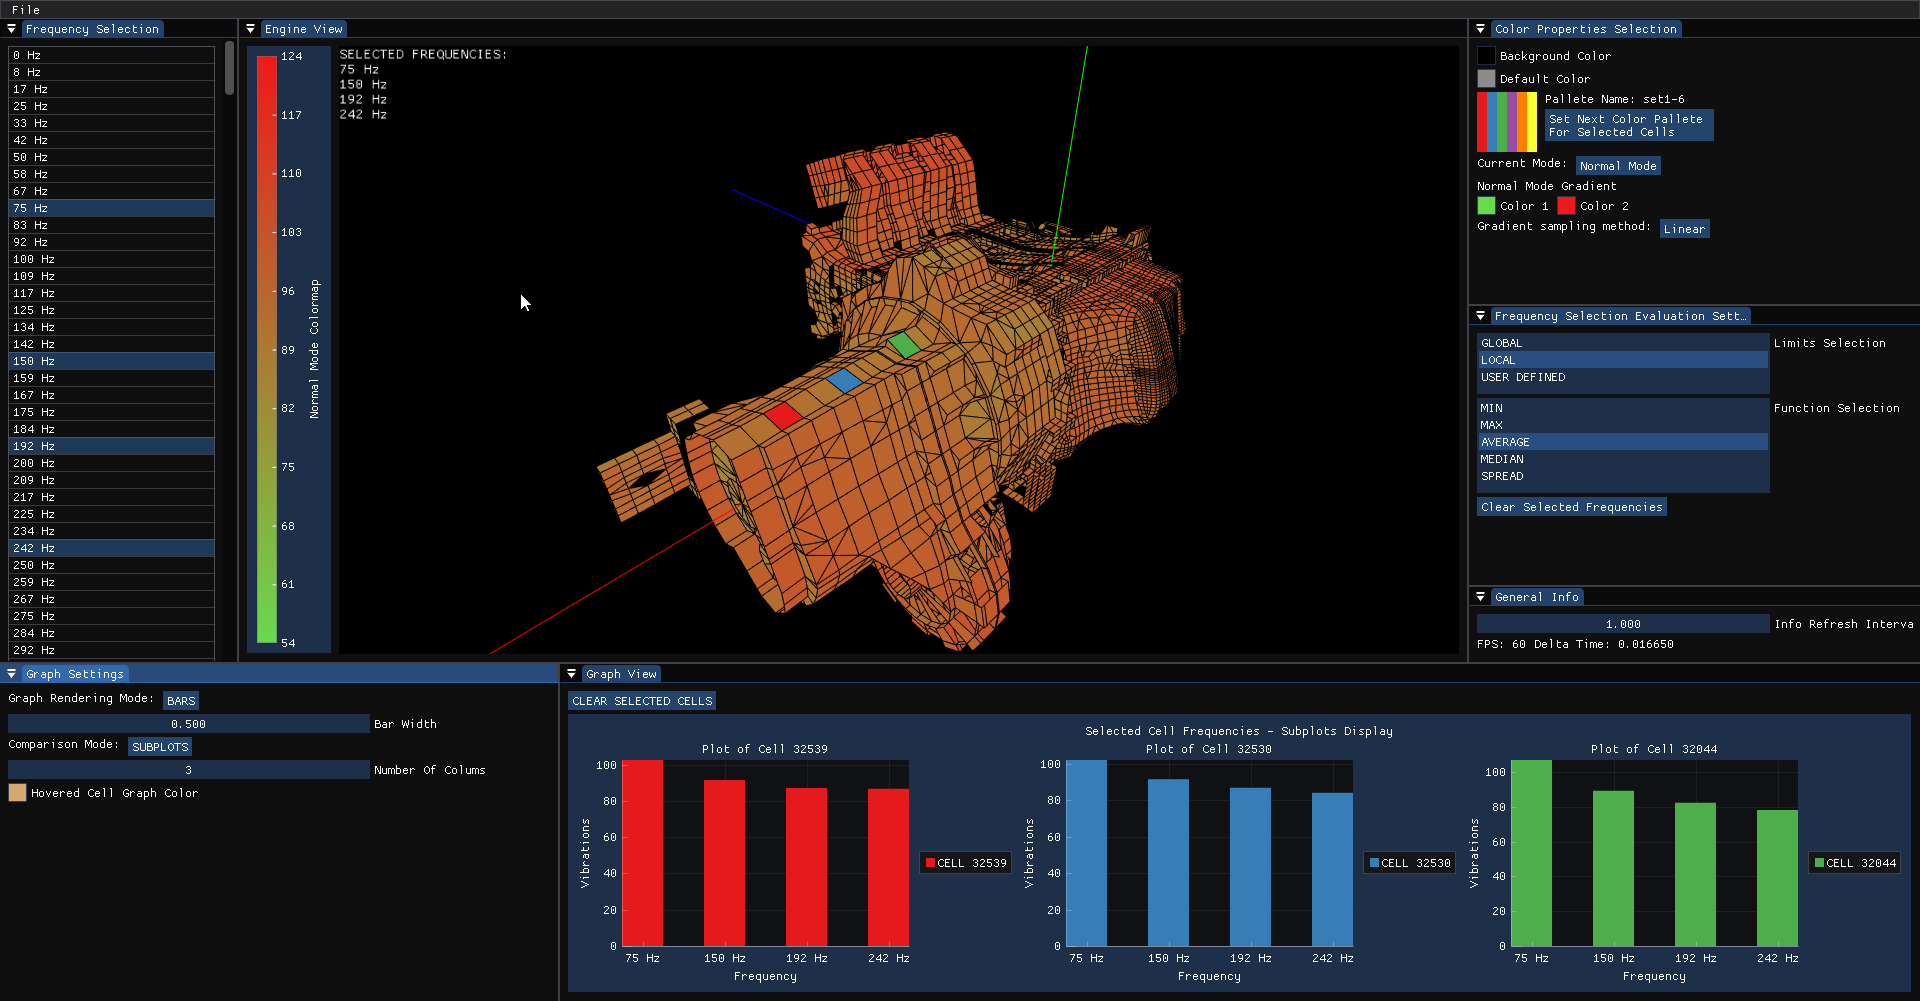
\includegraphics[width=\linewidth]{general_screenshot.png}
\caption{Snimka zaslona alata}
\label{fig:gen-screen}
\end{figure}

\section{Prikaz motora} \label{engine-view-section}
Zadaća prikaza motora je jasno vizualizirati podatke o vibracijama ćelija, pritom uzimajući u obzir brojne postavke vizualizacije poput: načina rada, odabranih frekvencija, načina računanja konačnih podataka ćelije, zadanih raspona podataka, gradijenata koje se koristi za vizualizaciju i načina uzorkovanja tih gradijenata. Korisnik ovu komponentu također može koristiti i za označavanje interesnih ćelija.\\
\begin{figure}[H]
\centering
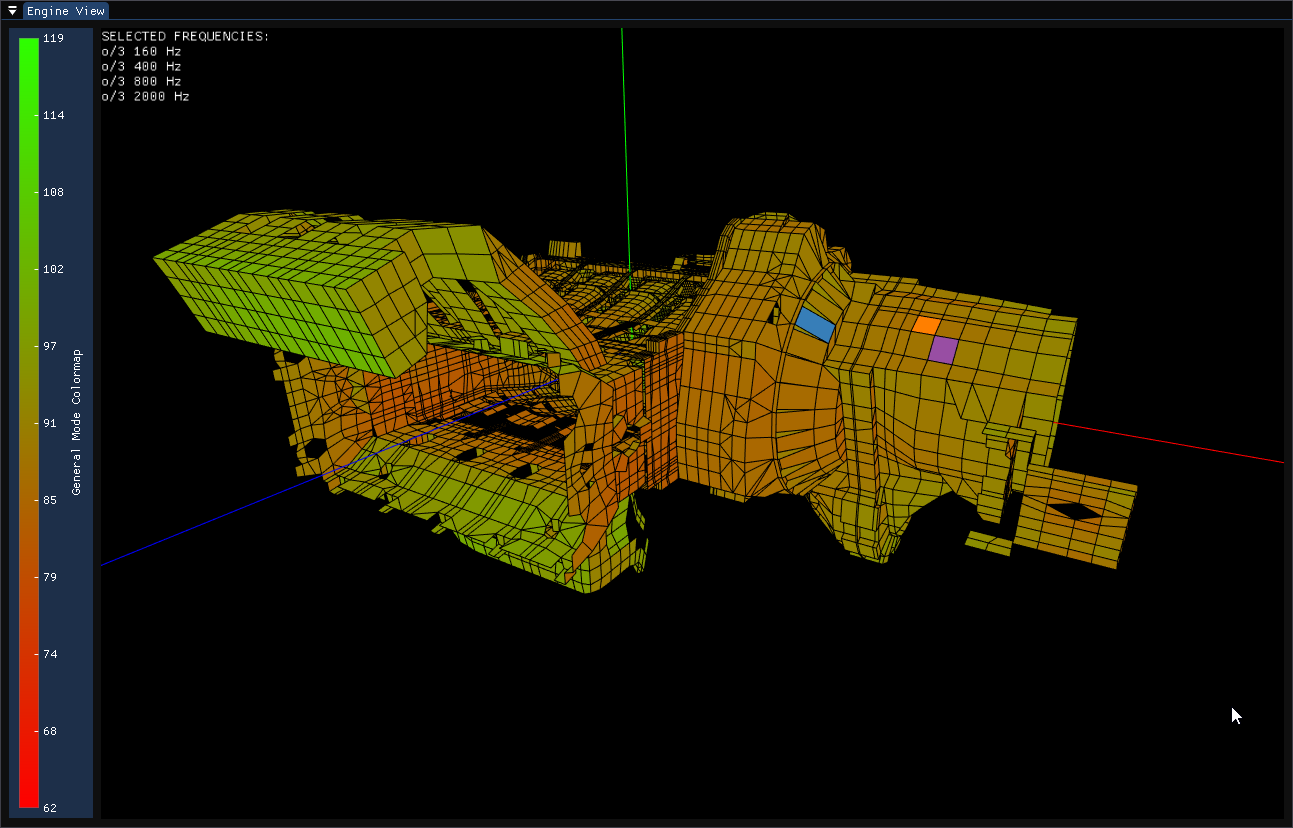
\includegraphics[width=0.85\linewidth]{engine_view_normal_mode.png}
\caption{Prikaz motora tijekom normalnog načina rada}
\label{fig:normal-mode-engine-view}
\end{figure}
\begin{figure}[h]
\centering
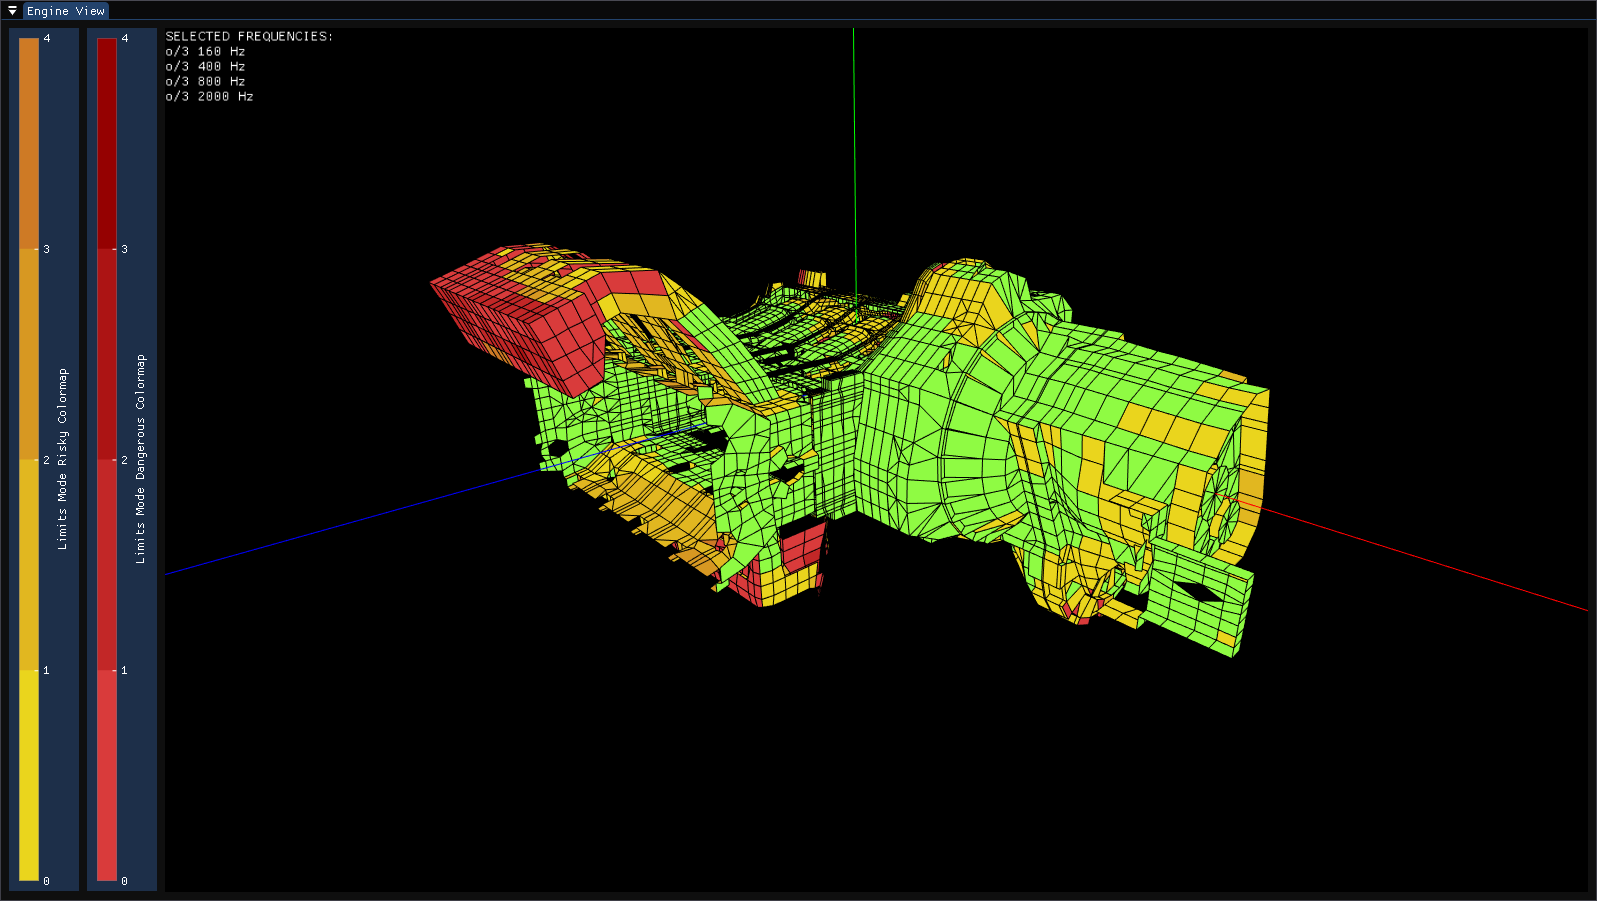
\includegraphics[width=0.85\linewidth]{engine_view_limits.png}
\caption{Prikaz motora tijekom načina rada s preddefiniranim ograničenjima}
\label{fig:limits-mode-engine-view}
\end{figure}

Na slikama \ref{fig:normal-mode-engine-view} i \ref{fig:limits-mode-engine-view} se može vidjeti primjer ovog prikaza tijekom dva moguća načina rada. Uz prikaz obojanog modela ova komponenta alata je zadužena i za prikaz legende gradijenta i nabrajanje odabranih frekvencija vibriranja, kako bi snimak prikaza prenosio sve relevantne informacije potrebne za razumijevanje rezultata vizualizacije. Osi koordinatnog sustava su nacrtane uz model motora kako bi korisnik dobio osjećaj za 3D prostor u kojem se model nalazi. Označavanje ćelija se odrađuje pozicioniranjem pokazivača miša iznad interesne ćelije te klikom na lijevu tipku miša. Kada korisnik pokazivačem miša prijeđe preko ćelije bez klikanja, boja ćelije postaje inverz prijašnje boje, kako bi se korisniku dala povratna informacija o ćeliji koja će biti odabrana odluči li se korisnik kliknuti lijevu tipku miša. Opisana ćelija će se u nastavku rada nazivati "lebdeća" ćelija. Jednom kada korisnik klikne na ćeliju, ćelija se označava jednom od boja iz trenutne palete (detaljno objašnjeno u poglavlju \ref{color-settings-section}) te je korisniku prikazan detaljan uvid u podatke označene ćelije putem prikaza grafa (vidi poglavlje \ref{graph-view-section}). Ponovnim klikom na već odabranu ćeliju, ćelija se briše iz liste odabranih ćelija.\\

Kao što je vidljivo iz slika \ref{fig:normal-mode-engine-view} i \ref{fig:limits-mode-engine-view}, razlike u dva načina rada se ne manifestiraju samo u vizualizaciji motora, već i u sučelju ovog prikaza. Naime, kako je objašnjeno u poglavlju \ref{requests-section}, u normalnom načinu rada alatu je potreban jedan kontinuirani gradijent, a u načinu rada s preddefiniranim ograničenjima su potrebna dva diskretna gradijenta.
\begin{figure} [H]
     \centering
     \begin{subfigure}[h]{0.16\textwidth}
         \centering
         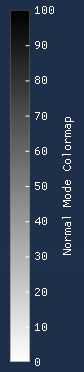
\includegraphics[width=\textwidth]{linear_colormap.png}
         \caption{Linearno}
         \label{fig:linear_legend}
     \end{subfigure}
     \hfill
     \begin{subfigure}[h]{0.16\textwidth}
         \centering
         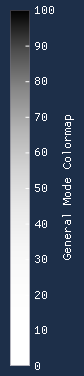
\includegraphics[width=\textwidth]{cubic_colormap.png}
         \caption{Kubno v1}
         \label{fig:cubic_legend}
     \end{subfigure}
     \hfill
     \begin{subfigure}[h]{0.16\textwidth}
         \centering
         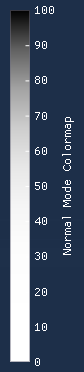
\includegraphics[width=\textwidth]{quartic_colormap.png}
         \caption{Kvartičko v1}
         \label{fig:quartic_legend}
     \end{subfigure}
     \hfill
     \begin{subfigure}[h]{0.16\textwidth}
         \centering
         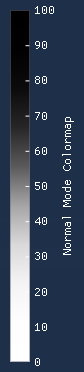
\includegraphics[width=\textwidth]{cubic_symmetrical_colormap.png}
         \caption{Kubno v2}
         \label{fig:cubic_symmetrical_legend}
     \end{subfigure}
     \hfill
     \begin{subfigure}[h]{0.16\textwidth}
         \centering
         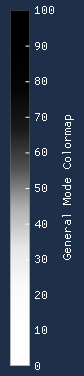
\includegraphics[width=\textwidth]{quartic_symmetrical_colormap.png}
         \caption{Kvartičko v2}
         \label{fig:quartic_symmetrical_legend}
     \end{subfigure}
        \caption{Drugačije postavke uzorkovanja gradijenta\\}
        \label{fig:colormap-legends}
\end{figure}

Osim što je navedene gradijente moguće mijenjati pomoću dvije kontrolne boje, moguće ih je mijenjati i promjenom funkcije uzorkovanja gradijenta, a utjecaj različitih funkcija uzorkovanja na kontinuirane gradijente se može vidjeti na slici \ref{fig:colormap-legends}. Različite funkcije uzorkovanja su izravno preuzete s web stranice Easing \citep{easing}.

\section{Prikaz grafa} \label{graph-view-section}

Komponenta prikaza grafa služi za iscrtavanje jednog ili više prikaza grafova odabranih ćelija, ali i "lebdeće" ćelije. Prilikom iscrtavanja spomenutih grafova uzimaju se u obzir brojne postavke i načini crtanja. Boje grafova odabranih ćelija odgovaraju bojama koje te ćelije imaju unutar prikaza motora (vidi poglavlje \ref{engine-view-section}), a boja grafa "lebdeće" ćelije je zadana unutar postavki grafa (vidi poglavlje \ref{graph-settings-section}). Kao što je navedeno u poglavlju \ref{requests-section}, alat implementira tri načina usporedbe i dva načina iscrtavanja grafova, a izgled ove komponente uz sve moguće kombinacije postavki grafa su prikazane na slikama u dodatku \ref{appendix:graph-display-examples}. Na navedenim slikama se može vidjeti kako ovu komponentu čini jedan ili više prikaza grafova i gumb za brisanje liste odabranih ćelija.\\

Sa slika u dodatku \ref{appendix:graph-display-examples} je također vidljivo kako su rasponi osi prikaza grafova postavljeni tako da obuhvaćaju podatke koji se u njima nalaze, te nisu fiksno određeni. Implementacija ovakvog načina određivanja raspona je odabrana zbog smanjene preglednosti razlika u "tokovima" grafova kada su postavljeni fiskni rasponi jer pri fiksnim rasponima grafovi zauzimaju puno manji dio prikaza, a ostatak prikaza je potrošen na prazan prostor. Spomenuta primjedba je posebno uočljiva na slikama \ref{appendix:subplots_graph_display_bars} i \ref{appendix:subplots_graph_display_lines} gdje se vidi kako, zbog različitih raspona, grafovi koji su iscrtani pomoću stupaca bolje pokazuju razliku u iznosima podataka, ali grafovi iscrtani pomoću linija bolje pokazuju razlike u "tokovima" grafova. Konkretno, na slici \ref{appendix:subplots_graph_display_bars} se na prvi pogled čini kako se zelena ćelija (ćelija 10982) i žuta ćelija (ćelija 11182) ponašaju slično, no uvidom u graf na slici \ref{appendix:subplots_graph_display_lines} se otkriva kako to nije istina. Ali ako se korisniku ovakav način određivanja raspona ne sviđa, u alatu je moguće otvoriti postavke bilo koje osi prikaza grafa pozicioniranjem pokazivača miša iznad željene osi te klikom na desnu tipku miša. Kao što se vidi na slici \ref{fig:graph-axis-settings}, unutar spomenutih postavki je moguće uređivati brojna svojstva osi poput raspona, načina interpoliranja između granica raspona, smjera osi i mnoge druge postavke.

\begin{figure} [H]
	\centering
    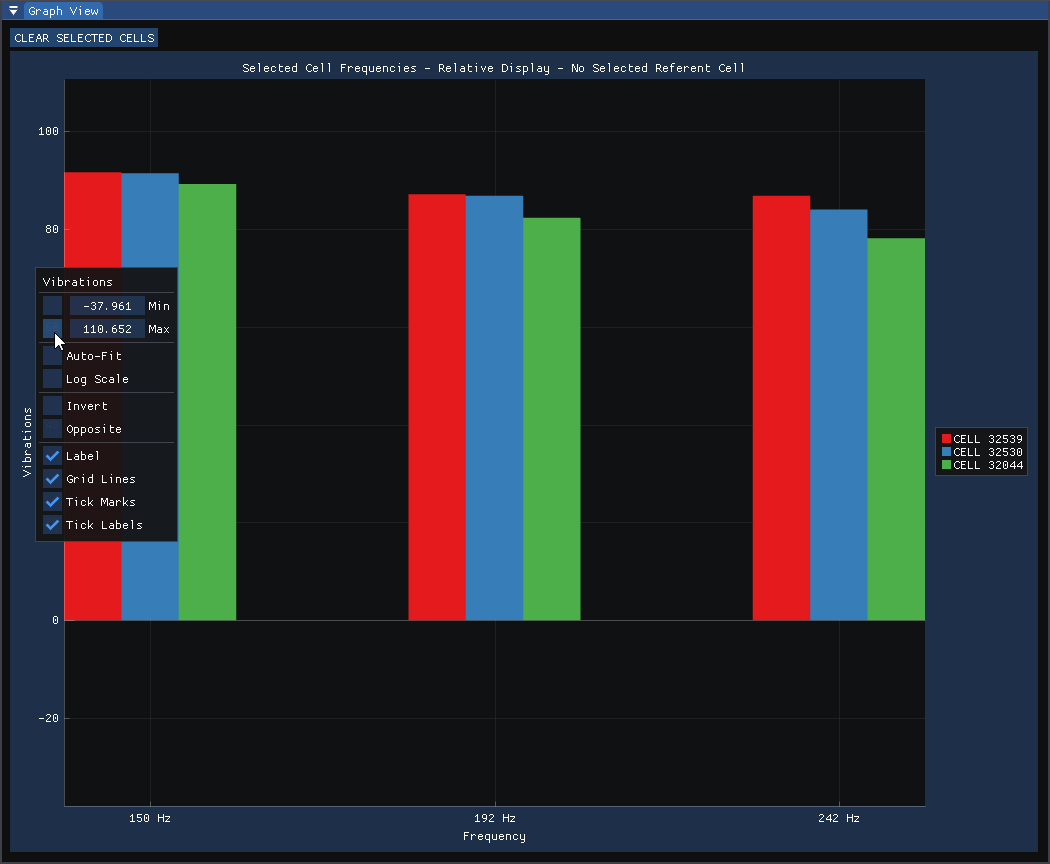
\includegraphics[width=\textwidth]{graph_view_axis_settings.png}
    \caption{Postavke osi prikaza grafa}
    \label{fig:graph-axis-settings}
\end{figure}

\section{Postavke boja} \label{color-settings-section}
Kao što samo ime ove komponente kaže, glavna svrha joj je čuvanje postavki koje bi mijenjale boje i gradijente unutar prikaza motora. Na slici \ref{fig:color-settings-2-modes} mogu se vidjeti razlike u komponenti između dva moguća načina rada. U oba načina rada moguće je promijeniti pozadinsku boju prikaza motora, početnu boju motora (boju koju motor ima kad nijedna frekvencija nije odabrana), paletu za odabrane ćelije i trenutni način rada. No dva prikaza postavki boja se ipak djelomično razlikuju jer je za normalni način rada potrebno definirati samo jedan gradijent, a za način rada s preddefiniranim ograničenjima je potrebno definirati jednu boju (za sigurnu zonu) i dva gradijenta (za rizičnu i opasnu zonu).

\begin{figure} [H]
     \centering
     \begin{subfigure}[h]{0.49\textwidth}
         \centering
         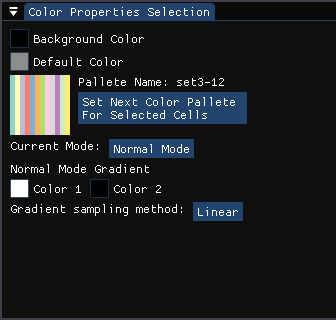
\includegraphics[width=\textwidth]{color_settings_normal_mode.png}
         \caption{Normalni način rada}
         \label{fig:color-settings-normal-mode}
     \end{subfigure}
     \hfill
     \begin{subfigure}[h]{0.49\textwidth}
         \centering
         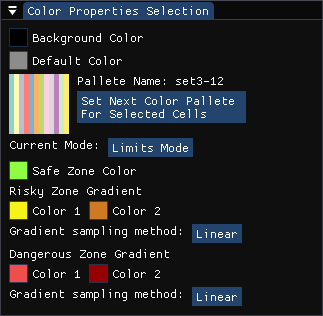
\includegraphics[width=\textwidth]{color_settings_limits_mode.png}
         \caption{Način rada s preddefiniranim ograničenjima}
         \label{fig:color-settings-limits-mode}
     \end{subfigure}
     \caption{Postavke boja tijekom dva moguća načina rada\\}
     \label{fig:color-settings-2-modes}
\end{figure}

Što se tiče mijenjanja postavki, korisnik može mijenjati boje klikom na obojani kvadrat čime se otvara prozor za mijenjanje boja prikazan na slici \ref{fig:color-picker}. U otvorenom prozoru boju se može mijenjati pomoću interaktivnog GUI sučelja ili unosom RGB ili HSV vrijednosti boje, a također je moguće i unošenje boja u heksadekadskom formatu.\\

\begin{figure} [H]
	\centering
    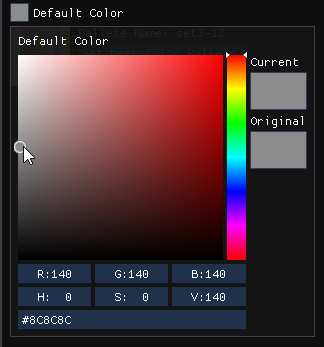
\includegraphics[width=0.5\textwidth]{color_settings_color_picker.png}
    \caption{Prozor za odabir boje\\}
    \label{fig:color-picker}
\end{figure}

Palete boja za odabrane ćelije su učitane izravno iz datoteke \textit{default\_pallete.txt} koja se mora nalaziti u istom direktoriju kao i izvršna datoteka alata. Početne palete su preuzete s web stranice ColorBrewer \citep{colorbrewer} i unesene su u navedenu datoteku u sljedećem formatu:

\begin{lstlisting}
p ime_palete
rgb_vrijednosti_boje1_u_rasponu_0_255
rgb_vrijednosti_boje2_u_rasponu_0_255
rgb_vrijednosti_boje3_u_rasponu_0_255
rgb_vrijednosti_boje4_u_rasponu_0_255
\end{lstlisting}
\ \\

Na slici \ref{fig:color-settings-2-modes} se može vidjeti kako je za svaku paletu u kvadratiću prikazan spektar boja, desno od kojeg je navedeno ime palete, a ispod imena se nalazi gumb za prelazak na sljedeću paletu. Kako palete sadrže ograničen broj boja, u alatu je implementiran način brisanja ćelija kada je broj odabranih ćelija veći od broja boja u paleti. Postoje dva slučaja kod kojih se to dogodi: pri dodavanju nove ćelije kada su već sve boje palete "zauzete" i pri mijenjanju trenutne palete na paletu čiji je broj boja manji od broja trenutno odabranih ćelija. U prvom slučaju alat briše zadnju odabranu ćeliju i dodaje novoodabranu ćeliju, a u drugom slučaju alat briše onoliko zadnjih odabranih ćelija kolika je razlika između broja odabranih ćelija i broja boja nove palete.\\

Ispod sučelja za mijenjanje palete se nalazi gumb za mijenjanje načina rada. Na gumbu piše ime trenutnog načina rada, a klikom na gumb alat prelazi u sljedeći način rada. Kako su moguća samo dva načina rada, gumb će alternirati između normalnog načina rada i načina rada s preddefiniranim ograničenjima.\\

Konačno, sučelje za odabir gradijenta se sastoji od dva standardna kvadrata za mijenjanje boja pomoću kojih se mijenja početna i krajnja kontrolna boja gradijenta. Ispod navedenih kvadrata se nalazi gumb za mijenjanje metode uzorkovanja gradijenta. Implementirane metode uzorkovanja i njihov utjecaj na gradijent su objašnjene i prikazane u poglavlju \ref{graph-view-section}.

\section{Postavke grafa} \label{graph-settings-section}

Postavke grafa se dijele na tri dijela koji su jasno naznačeni na slici \ref{fig:graph-settings-segmented}. Dio u kojem se mijenja boja grafa lebdeće ćelije se ne mijenja s obzirom na različite načine crtanja ili uspoređivanja jer se taj graf uvijek iscrtava. Kao što je već napomenuto u poglavlju \ref{requests-section}, alat implementira dva načina iscrtavanja grafa: linijski i stupčasti, a razlika u postavkama između ta dva načina je što stupčastom grafu korisnik može odrediti širinu stupca, kao što se može vidjeti na slici \ref{fig:graph-settings-segmented}, dok na linijskom grafu korisnik ne može mijenjati ništa. Način iscrtavanja se mijenja klikom na gumb na kojem piše ime trenutno aktivnog načina iscrtavanja.

\begin{figure} [H]
	\centering
    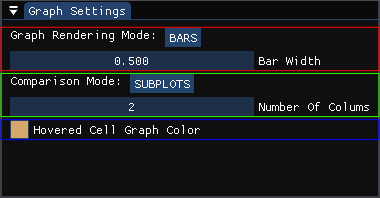
\includegraphics[width=0.7\textwidth]{graph_settings_subplots_segmented.png}
    \caption{Postavke grafa rastavljene na dijelove: postavke načina iscrtavanja (crveno), postavke načina usporedbe (zeleno) i postavke boje grafa "lebdeće ćelije" (plavo)}
    \label{fig:graph-settings-segmented}
\end{figure}

Ali za razliku od postavki načina iscrtavanja, razlike između postavki načina uspoređivanja su puno uočljivije. Tijekom normalnog načina usporedbe, korisnik nema nikakvih dodatnih postavki osim gumba za mijenjanje načina usporedbe koji je prisutan tijekom svih načina uspoređivanja i funkcionira na identičan način kao i gumb za mijenjanje načina iscrtavanja. Tijekom načina usporedbe s višestrukim prikazima, korisnik može odabrati u koliko će se stupaca prikazi organizirati. Konačno, kada je aktivan relativni način usporedbe, korisnik može odabrati jednu od već odabranih ćelija s obzirom na koju će se prikazati grafovi ostalih ćelija. Gumb ćelije koju korisnik odabere, ali i gumb ćelije iznad koje korisnik postavi pokazivač miša poprima boju odgovarajuće ćelije iz prikaza motora. Navedeni dodatak je implementiran kako bi korisnik imao bolju ideju o tome koja ćelija je trenutno odabrana i/ili koja će ćelija biti odabrana za relativno iscrtavanje.

\begin{figure} [H]
     \centering
     \begin{subfigure}[h]{0.48\textwidth}
         \centering
         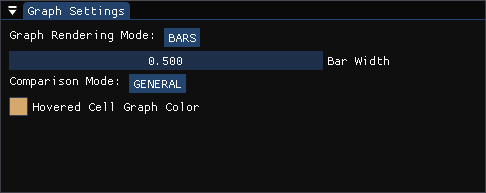
\includegraphics[width=\textwidth]{graph_settings_default.png}
         \caption{Normalni način usporedbe}
         \label{fig:graph-settings-normal-mode}
     \end{subfigure}
     \hfill
     \begin{subfigure}[h]{0.48\textwidth}
         \centering
         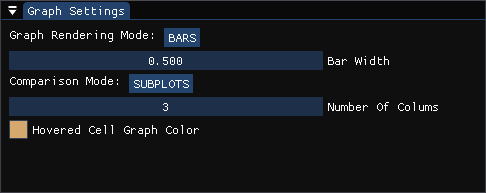
\includegraphics[width=\textwidth]{graph_settings_subplots.png}
         \caption{Način usporedbe s višestrukim prikazima}
         \label{fig:graph-settings-limits-mode}
     \end{subfigure}
     \hfill
     \begin{subfigure}[h]{0.48\textwidth}
         \centering
         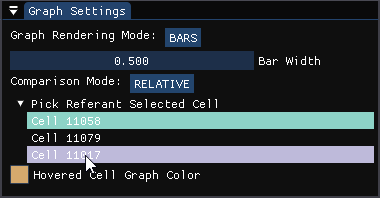
\includegraphics[width=\textwidth]{graph_settings_relative.png}
         \caption{Relativni način usporedbe}
         \label{fig:graph-settings-limits-mode}
     \end{subfigure}
     \caption{Postavke grafa tijekom tri različita načina usporedbe}
     \label{fig:graph-settings-3-modes}
\end{figure}

\section{Odabir frekvencija} \label{frequency-selection-section}

Ova komponenta služi isključivo za odabir frekvencija (kao što i samo ime govori), a postavljena je u odvojenu komponentu od postavki evaluacije odabranih frekvencija (opisanih u poglavlju \ref{frequency-settings-section}) radi poboljšanja lakoće korištenja alata. Izgled komponente se može vidjeti na slici \ref{fig:frequency-selection-view}. U normalnom načinu rada komponenta prikazuje sve frekvencije za koje su učitani podaci o vibriranju ćelija, dok su u načinu rada s preddefiniranim ograničenjima prikazane samo frekvencije za koje je definirano ograničenje u datoteci s ograničenjima. 

\begin{figure} [H]
	\centering
    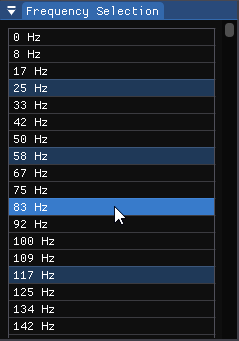
\includegraphics[width=0.45\textwidth]{frequency_selection_view.png}
    \caption{Prozor za odabir frekvencija}
    \label{fig:frequency-selection-view}
\end{figure}

\section{Postavke evaluacije odabranih frekvencija} \label{frequency-settings-section}

Kao što je već opisano u poglavlju \ref{requests-section}, korisnik u normalnom načinu rada može dodatno prilagoditi prikaz utjecaja odabranih frekvencija na snagu vibracije dijelova motora odabirom različitih metoda pomoću kojih se iz niza podataka o snazi vibracije ćelije dobije jedan konkretan podatak, ali i odabirom raspona pomoću kojeg se izračunati podatak pretvori u podatak iz raspona [0, 1] kako bi se olakšalo uzorkovanje gradijenta. Navedene prilagodbe nisu moguće prilikom načina rada s preddefiniranim ograničenjima jer je algoritam već "strogo" zadan i nema dijelova algoritma koje korisnik može mijenjati, ali spomenute parametre normalnog načina rada, korisnik može mijenjati unutar komponente postavki odabranih frekvencija koja je prikazana na slici \ref{fig:frq-sel-eval-settings}.

\begin{figure} [H]
	\centering
    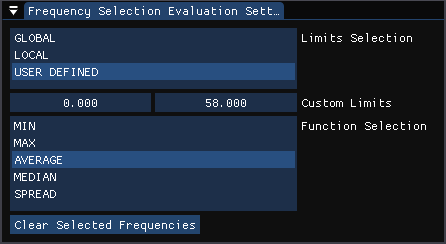
\includegraphics[width=0.8\textwidth]{frq_sel_eval_settings.png}
    \caption{Prozor postavki evaluacije odabranih frekvencija sa svim mogućim parametrima}
    \label{fig:frq-sel-eval-settings}
\end{figure}

Prozor postavki evaluacije odabranih frekvencija nije vidljiv sve dok korisnik ne odabere jednu od ponuđenih frekvencija unutar komponente iz poglavlja \ref{frequency-selection-section}. Kada se odabere barem jedna frekvencija, prozor postavki se prikazuje s parametrima koji su vidljivi ovisno o broju odabranih frekvencija i načinu rada u kojem korisnik koristi alat.\\

Oba načina rada u postavkama imaju gumb za brisanje liste trenutno odabranih frekvencija. Način rada s preddefiniranim ograničenjima osim tog gumba u postavkama neće imati niti jedan drugi element, a normalni način rada će moći mijenjati već spomenute metode računanja konačnih podataka i raspone izračunatih podataka. Lista za odabir raspona je vidljiva kada korisnik odabere barem jednu frekvenciju, a mijenjanje raspona definiranog od korisnika je omogućeno kada je navedeni raspon odabran u spomenutoj listi. Lista za odabir metoda računanja konkretnih podataka je vidljiva kada korisnik odabere dvije ili više frekvencije jer se pri jednoj odabranoj frekvenciji sve funkcije ponašaju identično.


\section{Općenite informacije}

Na slici \ref{fig:general-info} se može vidjeti komponenta koja služi za prikaz općenitih informacija vezanih za performanse alata poput broja sličica po sekundi i vremena proteklog između iscrtavanja dviju sličica. Korisnik dodatno može promijeniti interval nakon kojeg se navedene informacije ažuriraju.

\begin{figure} [H]
	\centering
    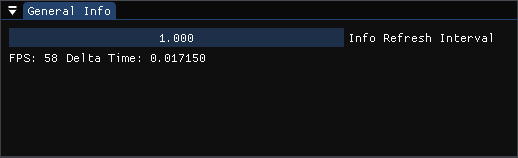
\includegraphics[width=0.9\textwidth]{general_info.png}
    \caption{Prozor za općenite informacije\\}
    \label{fig:general-info}
\end{figure}

\chapter{Implementacija}

Alat je razvijen u programskom jeziku C++ uz korištenje biblioteke OpenGL za komuniciranje s grafičkom karticom. No, osim OpenGL-a za razvoj alata je korišten i niz drugih biblioteka, čiji su detaljniji opisi i razlozi za korištenje navedeni u poglavlju \ref{libraries-section}. Budući da su se tijekom razvoja alata konstantno pojavljivali novi zahtjevi i funkcionalnosti koje se treba implementirati, bilo je potrebno uspostaviti arhitekturu rješenja koje će se rješenje pridržavati kako ne bi postalo kruto i krhko, a ta arhitektura je opisana u poglavlju \ref{codebase-architecture-section}. Konačno, kako je način slanja podataka s procesora na grafičku karticu iznimno važna komponenta izvedbe svake grafičke aplikacije, poglavlje \ref{graphics-card-data-section} opisuje kako je organiziran tok podataka s procesora na grafičku karticu.

\section{Korištene biblioteke} \label{libraries-section}

\subsection{OpenGL}

OpenGL \citep{opengl} je višeplatformska i višejezična biblioteka koja služi za prikazivanje 2D i 3D vektorske grafike. Biblioteka podržava dva distinktna načina rada: \textit{compatibility} i \textit{core}. U \textit{compatibility} načinu rada klijent definira poziciju i boju točaka primitiva koje želi iscrtati pozivajući funkcije API-a, nakon čega se navedene točke propuštaju kroz fiksni grafički protočni sustav na kraju kojega se iscrtava slika. \textit{Core} način rada, često zvani moderni OpenGL, dopušta klijentu mijenjanje određenih dijelova grafičkog protočnog sustava pomoću sjenčara \engl{shader}. Sjenčari su programi napisani u GLSL-u \engl{OpenGL Shading Language} koji se izvode na grafičkoj kartici, te manipuliraju podacima poslanim od strane klijenta preko OpenGL API-a u obliku tzv. \textit{buffer object}-a kako bi se postigli različiti vizualni efekti.\\

Za razvoj alata opisanog u ovom radu je korišten OpenGL 3.3 u \textit{core} načinu rada. Iako je u sklopu implementacije alata ova biblioteka prvenstveno korištena za iscrtavanje 3D modela motora, implementacije biblioteka Dear ImGui (poglavlje \ref{imgui-section}) i ImPlot (poglavlje \ref{implot-section}) korištene u ovom radu također koriste OpenGL za iscrtavanje elemenata korisničkog sučelja i 2D grafova.

\subsection{Dear ImGui} \label{imgui-section}
Dear ImGui \citep{imgui} je C++ biblioteka koja služi za iscrtavanje grafičkog korisničkog sučelja ili GUI-a \engl{Graphical User Interface}.\\

GUI biblioteke se obično mogu razvrstati na zadržane \engl{retained} i izravne \engl{immediate} s obzirom na korištene obrasce ažuriranja prikaza. Zadržane biblioteke interno čuvaju podatke o primitivima korisničkog sučelja koje treba iscrtati, a klijent pozivima metoda biblioteke ne može izravno utjecati na iscrtavanje tih primitiva, već jedino može mijenjati apstraktni model korisničkog sučelja. Na ovakav način zadržane biblioteke mogu dodatno optimizirati kako i kada će se izvršiti iscrtavanje elemenata. S druge strane, izravne GUI biblioteke omogućuju klijentu izravno pozivanje metoda za iscrtavanje elemenata korisničkog sučelja. Zbog toga klijent treba pozivati funkcije za iscrtavanje primitiva u svakoj iteraciji petlje ažuriranja aplikacije.\\

Dear ImGui spada u kategoriju izravnih GUI biblioteka. Ova biblioteka omogućuje jednostavno i brzo iteriranje GUI aplikacija, te unatoč tome što joj nedostaju određene funkcionalnosti koje se mogu naći u drugim GUI bibliotekama, i dalje je iznimno popularna u području razvoja GUI aplikacija zbog jednostavnosti korištenja i nadogradnje.

\subsection{ImPlot} \label{implot-section}

Iako Dear ImGui službeno podržava crtanje grafova, funkcionalnosti grafova implementiranih u sklopu ove biblioteke su iznimno ograničene. Iz tog razloga, za implementaciju grafova u ovom radu je korištena biblioteka ImPlot \citep{implot}. Ova biblioteka je proširenje Dear ImGui-a koje omogućava prikaz raznovrsnih interaktivnih grafova jednostavnim izravnim pozivima metoda za iscrtavanje. 

\subsection{Ostale biblioteke}
Osim već spomenutih biblioteka, za razvoj ovog alata je korištena još nekolicina drugih biblioteka koje su navedene u ovom poglavlju.\\

GLFW \citep{glfw} je višeplatformska biblioteka za razvoj OpenGL aplikacija, a u sklopu ove aplikacije biblioteka je korištena za stvaranje prozora, konteksta, javljanje događaja i primanje ulaza od korisnika.\\

GLM \citep{glm} je matematička biblioteka za grafičke aplikacije pisane u OpenGL-u. GLM nudi brojne klase i funkcije koje su dizajnirane i implementirane s istim konvencijama imenovanja i funkcionalnostima kao odgovarajući tipovi podataka i funkcije u GLSL-u. GLM je u ovom alatu korišten za operacije nad vektorima, te računanje matrica transformacije i projekcije.\\

NFD \citep{nfd} \engl{Native File Dialog} je višeplatformska C biblioteka koja pruža mogućnost otvaranja izvornog dijaloga za datoteke, a u sklopu alata je korištena prilikom učitavanja različitih datoteka s podacima o motoru.

\section{Arhitektura rješenja} \label{codebase-architecture-section}

Organizacija k\^{o}da alata je generalno inspirirana obrascom Model-Pogled-Upravljač ili MVC \engl{Model-View-Controller} kako bi se omogućilo lakše održavanje programa. Na slici \ref{fig:high-level-overview} se može vidjeti pojednostavljeni prikaz MVC organizacije alata s većinom ključnih klasa alata.

\begin{figure} [H]
	\centering
    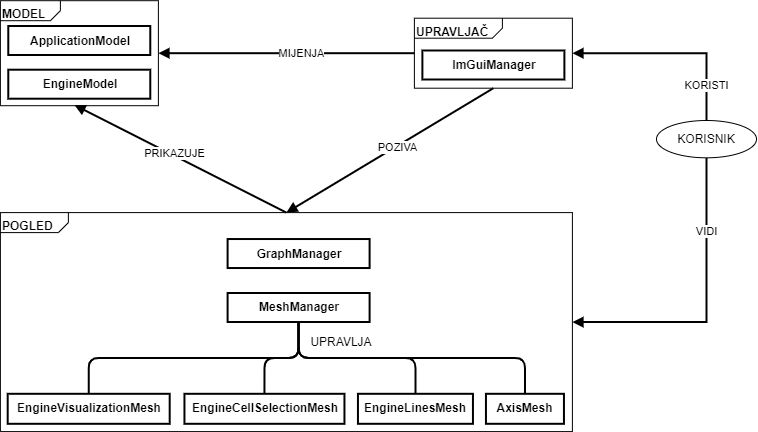
\includegraphics[width=\textwidth]{high_level_overview.png}
    \caption{Pregled MVC organizacije alata}
    \label{fig:high-level-overview}
\end{figure}
\ 
\\

Važno je spomenuti kako na slici \ref{fig:high-level-overview} nedostaje glavna klasa alata, a to je klasa \textit{App} jer ne sudjeluje izravno u MVC arhitekturi. Glavna odgovornost ove klase je povezivanje prikazanih komponenti, obrađivanje GLFW događaja i pozivanje metoda za ažuriranje spomenutih komponenti tijekom iteracija petlje ažuriranja. Spomenuta klasa stvara instance komponenti MVC arhitekture, te ih međusobno povezuje slanjem preko argumenata konstruktora ili povezivanjem preko sustava događaja i signala (detaljno opisanih u dodatku \ref{appendix:event-signal-system}). U poglavljima koje slijede su opisane uloge, odgovornosti i dijelovi svake komponente MVC organizacije ovog alata.

\subsection{Model}
Osnovna odgovornost svakog Modela u sklopu MVC arhitekture je čuvanja podataka aplikacije i pravila za njihovu manipulaciju. Radi lakšeg razumijevanja k\^{o}da i raspodjele odgovornosti, Model ovog alata je podijeljen u dvije klase: \textit{EngineModel} i \textit{ApplicationModel}. Objekt klase \textit{EngineModel} čuva postavke i podatake vezane za motor i prikaz motora, poput odabranih frekvencija, odabranih ćelija, "trenutne" lebdeće ćelije, pozicija točaka motora, ćelija motora itd., te definira metode za mijenjanje navedenih podataka. S druge strane, odgovornost klase \textit{ApplicationModel} je čuvanje postavki aplikacije koje nisu izravno vezane za podatke o motoru ili prikaz tih podataka, te definiranje metoda za vanjsko mijenjanje tih postavki. Spomenute postavke i podaci uključuju razne postavke grafova, postavke bojanja motora, pozadinsku boju alata te poziciju i rotaciju kamere.\\

Navedene klase nemaju izravne reference na nijedan drugi dio MVC arhitekture, stoga svaki put kada se dogodi promjena u Modelu, oni je javljaju "pretplatnicima" na tu promjenu pomoću događaja i/ili signala, čime se smanjuje krutost programskog rješenja. Što se mijenjanja postavki tiče, objekti spomenutih klasa interno sadrže objekte klase \textit{VariableMap}, čija je odgovornost čuvanje varijabli postavki, te pozivanje zadane metode kada se dogodi promjena u nekoj varijabli. Na taj način su omogućeni povratni pozivi, koje Dear ImGui za većinu elemenata korisničkog sučelja zapravo ne podržava. Kako bi se promjene u Modelu ispitale prilikom svake iteracije petlje ažuriranja alata, već spomenuta klasa \textit{App} poziva odgovarajuće metode objekata klasa \textit{EngineModel} i \textit{ApplicationModel} koje interno zovu metode vlastitih \textit{VariableMap} objekata.

\subsection{Pogled} \label{view-section}
Pogled je, kao komponenta MVC-a, uglavnom odgovoran za prikaz podataka komponente Model na koristan i praktičan način. Na slici \ref{fig:high-level-overview} se može vidjeti kako je komponenta Pogled, baš kao i Model, implementirana pomoću dvije klase: \textit{MeshManager} i \textit{GraphManager}.\\

Ključna odgovornost klase \textit{MeshManager} je iscrtavanje poligona i linija uz pomoć OpenGL-a na temelju podataka iz komponente Model. Kako se može vidjeti na skici organizacije arhitekture k\^{o}da, klasa \textit{MeshManager} ovu odgovornost razlaže na četiri dodatne klase: \textit{EngineVisualizationMesh}, \textit{EngineCellSelectionMesh}, \textit{EngineLinesMesh} i \textit{AxisMesh}. Navedene klase nasljeđuju apstraktnu klasu \textit{AbstractMesh}, s time da sve klase osim klase \textit{AxisMesh} klasu ne nasljeđuju izravno, već preko apstraktne klase \textit{AbstractEngineMesh}.
Implementirana je i klasa \textit{Shader} kako bi se apstrahirale operacije vezane za sjenčare, pa svaka od spomenutih komponenata \textit{MeshManager}-a sadrži vlastitu instancu klase \textit{Shader} i definira vlastite \textit{buffer object}-e koje šalje na grafičku karticu (više u poglavlju \ref{graphics-card-data-section}). Klasa \textit{App} u svakoj iteraciji petlje ažuriranja pozove metodu \textit{render} klase \textit{MeshManager} čija je odgovornost ažuriranje prikaza modela motora u stvarnom vremenu.\\

Rezultati iscrtavanja se ne spremaju izravno u glavni grafički međuspremnik \engl{framebuffer}, već u dva sporedna međuspremnika. U prvi međuspremnik rezultate iscrtavanja upisuju objekti klasa \textit{EngineVisualizationMesh}, \textit{EngineLinesMesh} i \textit{AxisMesh}. Klasa \textit{EngineVisualizationMesh} računa boje ćelija pomoću podataka iz Modela te iscrtava "obojani" motor. Klasa \textit{EngineLinesMesh} iscrtava linije koje obrubljuju ćelije kako bi se lakše prepoznale njihove granice, a klasa \textit{AxisMesh} služi za iscrtavanje koordinatnih osi kako bi korisnik dobio osjećaj za 3D prostor u kojem se motor nalazi. Opisani grafički međuspremnik se prikazuje korisniku tako što se u prikazu motora zapravo crta tekstura u koju se spremaju RGB vrijednosti međuspremnika. Drugi međuspremnik se koristi isključivo za prepoznavanje trenutne "lebdeće" ćelije, pa je "skriven" od korisnika. Razlika između ovog međuspremnika i međuspremnika vidljivog korisniku je što su ćelije motora u ovom međuspremniku konstantno obojane istim bojama koje ovise isključivo o indeksu ćelije. Stoga se u svakom trenutku ovaj grafički međuspremnik može uzorkovati na pikselu na kojem se nalazi pokazivač miša kako bi se iz dobivene RGB vrijednosti piksela saznao indeks ćelije na kojoj je pokazivač miša pozicioniran. Iscrtavanje ovih podataka u "skriveni" međuspremnik, te uzorkovanje istog je zadatak klase \textit{EngineCellSelectionMesh}. Razlike između prikaza ovih međuspremnika su vidljive na slici \ref{fig:framebuffers-example}.

\begin{figure} [H]
     \centering
     \begin{subfigure}[h]{0.8\textwidth}
         \centering
         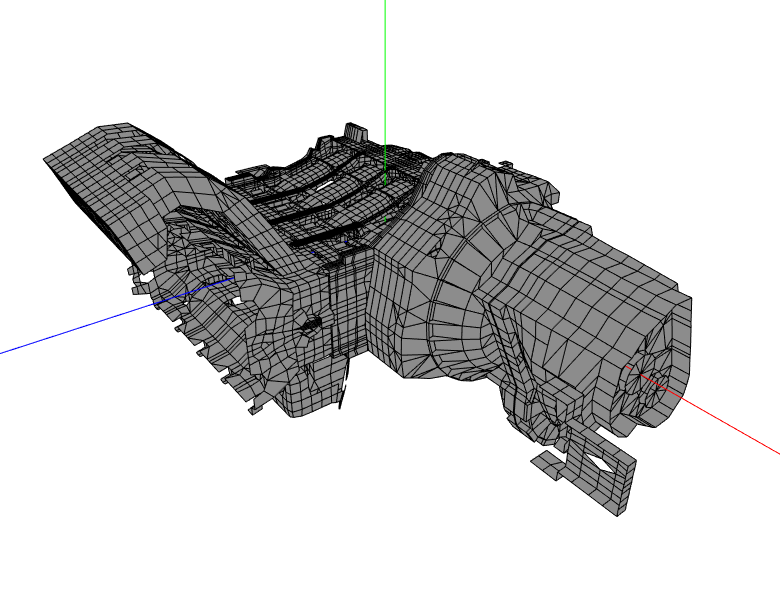
\includegraphics[width=\textwidth]{engine_default_color.png}
         \caption{Grafički međuspremnik koji je vidljiv korisniku}
         \label{fig:color-settings-normal-mode}
     \end{subfigure}
     \hfill
     \begin{subfigure}[h]{0.8\textwidth}
         \centering
         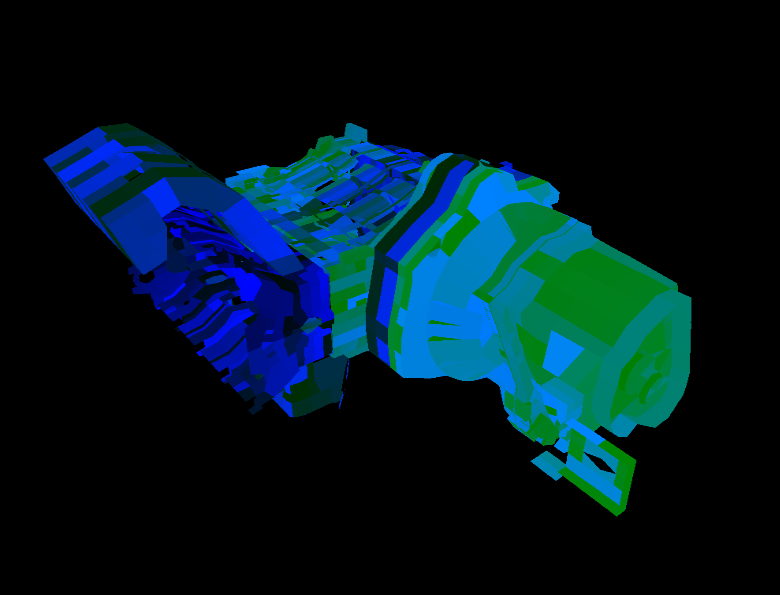
\includegraphics[width=\textwidth]{engine_cell_selection.png}
         \caption{Grafički međuspremnik za detekciju "lebdeće" ćelije}
         \label{fig:color-settings-limits-mode}
     \end{subfigure}
     \caption{Razlike između prikaza grafičkih međuspremnika}
     \label{fig:framebuffers-example}
\end{figure}

Druga klasa koja čini komponentu Pogleda je \textit{GraphManager}, a njena odgovornost je prikaz 2D grafova i legende gradijenta s obzirom na podatke koji su dostupni u Modelu poput: odabranih postavki, frekvencija i ćelija. Instanca ove klase izravno poziva metode biblioteke ImPlot koje su dodatno izmijenjene kako bi se omogućilo eksplicitno definiranje boja koje se koriste za crtanje grafova i legende gradijenta preko argumenata metoda. Klasa se pretplaćuje na događaje i signale Modela, tj. instanci sastavnih klasa Modela, koji su relevantni za ažuriranje instance pomoćne klase \textit{GraphData} unutar koje se čuvaju podaci važni za iscrtavanje grafova. Na ovaj način se objekt klase \textit{GraphData} ne mora ponovno "puniti" podacima u svakoj iteraciji petlje ažuriranja. No, \textit{GraphManager} izravno dohvaća podatke Modela, tj. ne pretplaćuje se na promjene, koji mijenjaju izgled grafa, ali ne zahtjevaju ponovno postavljanje objekta klase \textit{GraphData}. Konkretne metode iscrtavanja i uspoređivanja grafova, te uzorkovanja legende gradijenta su implementirane pomoću obrasca Strategija, čime se olakšava potencijalno dodavanje novih metoda iste namjene. Za razliku od do sada objašnjenih klasa, klasa \textit{App} ne poziva direktno metodu za iscrtavanje grafova i legendi klase \textit{GraphManager}, već to radi klasa \textit{ImGuiManager} kada definira prikaze korisničkog sučelja alata unutar kojih se te komponente trebaju nalaziti.\\

\subsection{Upravljač}

Komponenta Upravljač je u arhitekturi MVC uvijek odgovorna za komunikaciju s korisnikom, a kako je većina spomenute komunikacije u ovom alatu omogućena pomoću korisničkog sučelja koje pruža biblioteka Dear ImGui, glavna komponenta Upravljača je klasa \textit{ImGuiManager}. Navedena klasa je odgovorna za sve pozive metoda koje su dio biblioteke Dear ImGui, stoga ova klasa definira prozore korisničkog sučelja i njihove sadržaje, gumbe i funkcije koje se pozivaju na aktivaciju gumba, sučelja za mijenjanje boja i brojeva, izbornike i dijaloge za učitavanje datoteka itd. Osim navedenog, dužnost ove klase je i obavještavanje ostalih komponentama o događajima koji su vezani za korisničko sučelje poput promjene veličine prikaza motora ili definiranje direktorija datoteke za učitavanje podataka o motoru. Instanca ove klase čuva pokazivač na objekt klase \textit{MeshManager} kako bi pristupila teksturi u koju je spremljen grafički međuspremnik koji se prikazuje korisniku (opisan u poglavlju \ref{view-section}). Spomenutu teksturu zatim može prikazati u prozoru zaduženom za prikaz motora. Uz to instanca klase \textit{ImGuiManager} čuva i pokazivač na objekt klase \textit{GraphManager} čije metode koristi za iscrtavanje grafova i legende gradijenta.\\

Važno je naglasiti kako, unatoč tome što je veliki dio interakcije s korisnikom u alatu implementiran pomoću biblioteke Dear ImGui, veliki dio stvarne interakcije koju korisnik obavlja s alatom nije vezan za dijelove korisničkog sučelja već za događaje poput klika i kretanja miša, te pomicanja kotačića miša. Ti su događaji važni kako bi se korisniku omogućilo označavanje "lebdeće" ćelije, odabiranje "lebdeće" ćelije i kontrola kamere. Kako je već spomenuto na početku poglavlja \ref{codebase-architecture-section}, klasa \textit{App} zapravo obrađuje GLFW događaje koji javljaju ovakav tip korisničkog unosa. Budući da su takvi događaji \textit{ImGuiManager}-u važni za obraditi, objekt klase \textit{App} prvo pozove metodu objekta klase \textit{ImGuiManager} koja je zadužena za obrađivanje specifičnog događaja. U spomenutoj metodi se obrađivanje događaja delegira biblioteci Dear ImGui, a zatim se ispita je li pokazivač miša iznad prikaza modela motora, pošto su sve navedene interakcije vezane za prikaz modela motora. \textit{ImGuiManager} vraća odgovor na taj upit preko povratne vrijednosti pozvane funkcije. Ako je pokazivač miša iznad prikaza motora u trenutku pojave događaja, objekt klase \textit{App} će događaj dodatno obraditi pomoću ostalih komponenti MVC arhitekture, tako da je na neizravan način i klasa \textit{App} dio komponente Upravljač.


\section{Organizacija podataka na grafičkoj kartici} \label{graphics-card-data-section}

U poglavlju \ref{view-section} je objašnjeno kako četiri klase šalju vlastitim sjenčarima različite podatke na grafičku karticu budući jer imaju različite uloge. Cilj ovog poglavlja je detaljnije objašnjavanje toka podataka između procesora i grafičke kartice za svaku od navedenih klasa, a kako bi se omogućilo što razumljivije objašnjavanje tog toka, važno je objasniti nekoliko generalnih razlika između načina slanja i iscrtavanja podataka korištenih u ovom alatu.\\

U alatu razvijenom u sklopu ovog rada se podaci na grafičku karticu šalju na dva načina: pomoću  \textit{vertex buffer object}-a i pomoću uniformnih varijabli. \textit{Vertex buffer object}-i, skraćeno VBO, sadrže polje podataka koji opisuju svaki vrh modela na način koji je relavantan sjenčaru vrhova. U grafičkom protočnom sustavu sjenčar vrhova procesira elemente VBO-a, a rezultate prosljeđuje u daljnji dio protočnog sustava. Za jedan sjenčar se može definirati proizvoljan broj VBO-a samo je važno uvijek povezati strukturu elementa koji je sačuvan u VBO-u s atributima sjenčara vrhova pomoću funkcija OpenGL-a poput \textit{glVertexAttribPointer}. Uniformne varijable su iste za svaki vrh, te su zajedničke sjenčaru vrhova i fragmenata. Njih klijent ne šalje na grafičku karticu učitavanjem u VBO-e, već izravnim definiranjem lokacije i "pakirane "vrijednosti uniformne varijable. Klijent saznaje lokaciju uniformne varijable u sjenčaru pozivanjem funkcije \textit{glGetUniformLocation} kojoj kao argumente predaje indeks sjenčara i ime uniformne varijable.\\

Također, u alatu se koriste i dvije različite metode za iscrtavanje podataka učitanih u VBO: \textit{glDrawArrays} i \textit{glDrawElements}. Metoda \textit{glDrawArrays} svaki element VBO-a šalje jednom u sjenčar vrhova, te pretpostavlja da su vrhovi unutar VBO-a poredani slijedno i prate strukturu koju predstavljaju, npr. tri vrha iz istog trokuta su unutar VBO-a definirani jedan za drugim, te zadnji trokut neće imati broj vrhova koji nije djeljiv s tri. S druge strane metoda \textit{glDrawElements} zahtjeva dodatno definirani \textit{buffer object} zvani \textit{element buffer object}, skraćeno EBO, unutar kojeg su spremljeni indeksi podataka iz VBO-a koji definiraju poredak iscrtavanja učitanih podataka. Korištenjem ove metode u slučaju kada lica modela imaju velik broj dijeljenih vrhova, značajno se smanjuje broj podataka koji se šalje preko VBO-a jer se podaci ponavljajućih vrhova mogu "reciklirati" višestrukim navođenjem indeksa tog vrha unutar EBO-a.

\subsection{Podaci za bojanje ćelija}

Podaci koji su relevantni za bojanje ćelija su organizirani u dva VBO-a i 4 uniformne varijable. Preko VBO-a, tj. podataka koji opisuju pojedini vrh, se šalju pozicije vrhova, indeks ćelije kojoj pripadaju i boja te ćelije. Ti podaci su rastavljeni u dva VBO-a na način da se pozicije i indeks ćelije vrha šalju u sklopu jednog VBO-a, a boja ćelije pomoću drugog. Na taj način se podaci koji su konstantni (pozicija i indeks ćelije) ne moraju slati svaki put kada se mijenjaju boje modela motora, već se šalju samo kad se učitaju iz datoteka.\\

Uniformne varijable koje se šalju na karticu za potrebe bojanja ćelija su matrice modela, pogleda i projekcije, te indeks trenutne "lebdeće" ćelije. Matrica modela je konstantno postavljena na matricu identiteta, a matrice pogleda i projekcije su tu kako bi se model pravilno iscrtavao i nakon promjene rotacije i pozicije kamere, te promjene dimenzija prozora prikaza motora. Indeks trenutne lebdeće ćelije je poslan kako bi sjenčar znao kojoj ćeliji treba postaviti boju na inverz trenutne boje. Na taj način nije potrebno ažurirati VBO s bojama ćelija svaki put kada pokazivač miša bude postavljen na novu ćeliju.\\

Za iscrtavanje ovih podataka se koristi metoda \textit{glDrawElements}, tako da je uz slanje podataka, potrebno poslati i indekse koji definiraju po kojem poretku ti podaci dolaze. Iako se na prvi pogled može primjetiti kako ćelije ne dijele vrhove s istim indeksom ćelija, važno je napomenuti kako OpenGL u \textit{core} načinu rada podržava samo iscrtavanje trokuta. Stoga ćelije koje su četverokuti treba podijeliti na trokute, a takve ćelije korištenjem metode \textit{glDrawElements} ne definiraju unutar VBO-a više šest točaka već četiri. Kako takve ćelije čine ukupno 90.191\% svih ćelija modela motora koji se koristi u ovom radu (ostatak ćelija su trokuti), primjenom ove optimizacije se na grafičku karticu šalje 31.614\% manje podataka o vrhovima.

\subsection{Podaci za detekciju lebdeće ćelije}

Podaci koji se koriste za iscrtavanje motora s ćelijama jedinstvenih boja (opisano u poglavlju \ref{view-section}) se na grafičku karticu šalju pomoću jednog VBO-a koji za svaki vrh definira njegovu poziciju i indeks ćelije kojoj pripada, te pomoću tri uniformne varijable: matrica modela, pogleda i projekcije. Sjenčar iz indeksa ćelije izračuna boju vrha te ćelije, a klasa \textit{EngineCellSelectionMesh} obavlja inverznu operaciju nakon što uzorkuje boju na pikselu iznad kojeg je postavljen pokazivač miša. Za ovo iscrtavanje se također koristi metoda \textit{glDrawElements}, te je smanjenje broja podataka jednako kao i kod podataka za bojanje ćelija.

\subsection{Podaci za linije ćelija}

Podaci koji se koriste za crtanje linija koje razgraničavaju ćelije se na grafičku karticu šalju pomoću jednog VBO-a koji prenosi samo pozicije vrhova linija i tri uniformne varijable koje su matrice modela, pogleda i projekcije. Ovi podaci se također iscrtavaju pomoću metode \textit{glDrawElements} od koje dobivaju veću uštedu u odnosu na korištenje metode \textit{glDrawArrays} jer se pozicije vrhova mogu dijeliti između ćelija.

\subsection{Podaci za koordinatne osi}
Za crtanje linija koordinatnih osi se koristi jedan VBO unutar kojeg se prenosi polje podataka o vrhovima koji su opisani u dva bajta: prvi bajt je indeks u rasponu od 0 do 3, te služi za identificiranje pozicije vrha koordinatnih osi (točka ishodišta ili vrh x/y/z osi), a drugi bajt je indeks u rasponu od 0 do 2 i definira kojoj osi taj vrh pripada. Sjenčar interno definira konstantna polja koja indeksira pomoću indeksa iz VBO-a. Osim VBO-a sjenčar prima i dvije uniformne varijable: matrice pogleda i projekcije. Za razliku od dosadašnjih podataka, ovi podaci se crtaju metodom \textit{glDrawArrays}. Ova metoda se koristi zbog jednostavnosti i manje količine potrebnih podataka u odnosu na metodu \textit{glDrawElements}, koja bi zahtijevala dodatno definiranje EBO-a, što za ovako mali broj vrhova nema smisla.

\chapter{Demonstracija rada alata}

\section{Učitavanje datoteka}

Kada korisnik prvi put pokrene alat, prozori alata će izgledati slično kao na slici \ref{fig:initial-screenshot}. Važno je naglasiti kako korisnik može promijeniti poziciju i veličinu svakog prozora u sklopu alata, a ta promjena će ostati spremljena nakon zatvaranja alata.

\begin{figure} [H]
	\centering
    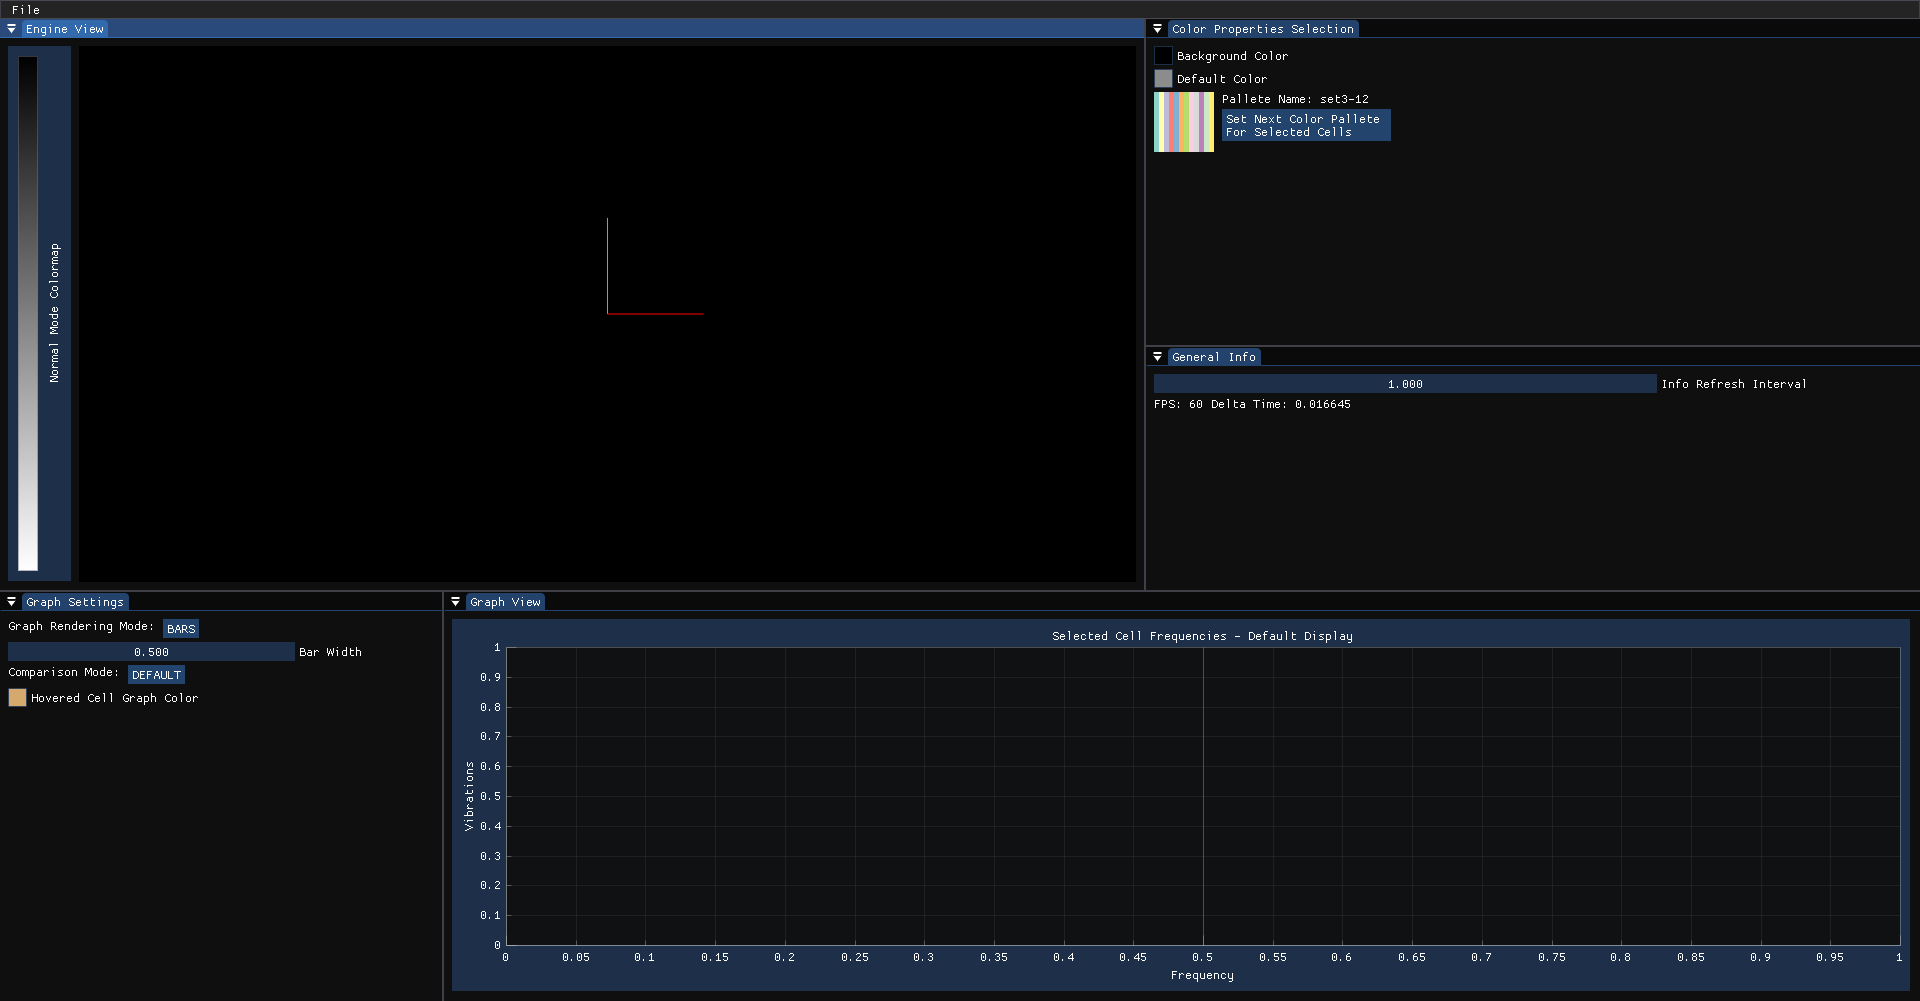
\includegraphics[width=\textwidth]{demonstration/initial_screenshot.png}
    \caption{Prikaz alata nakon pokretanja}
    \label{fig:initial-screenshot}
\end{figure}

Kako bi korisnik mogao vizualizirati podatke s kojima su vibracije ćelija opisane, potrebno je učitati datoteke s relevantnim podacima. Navedene datoteke se mogu učitati pomoću izbornika prikazanog na slici \ref{fig:file-menu}. Klikom na bilo koji gumb tog izbornika se otvara izvorni dijalog za odabiranje datoteka prikazan na slici \ref{fig:file-dialog}.

\begin{figure} [H]
	\centering
    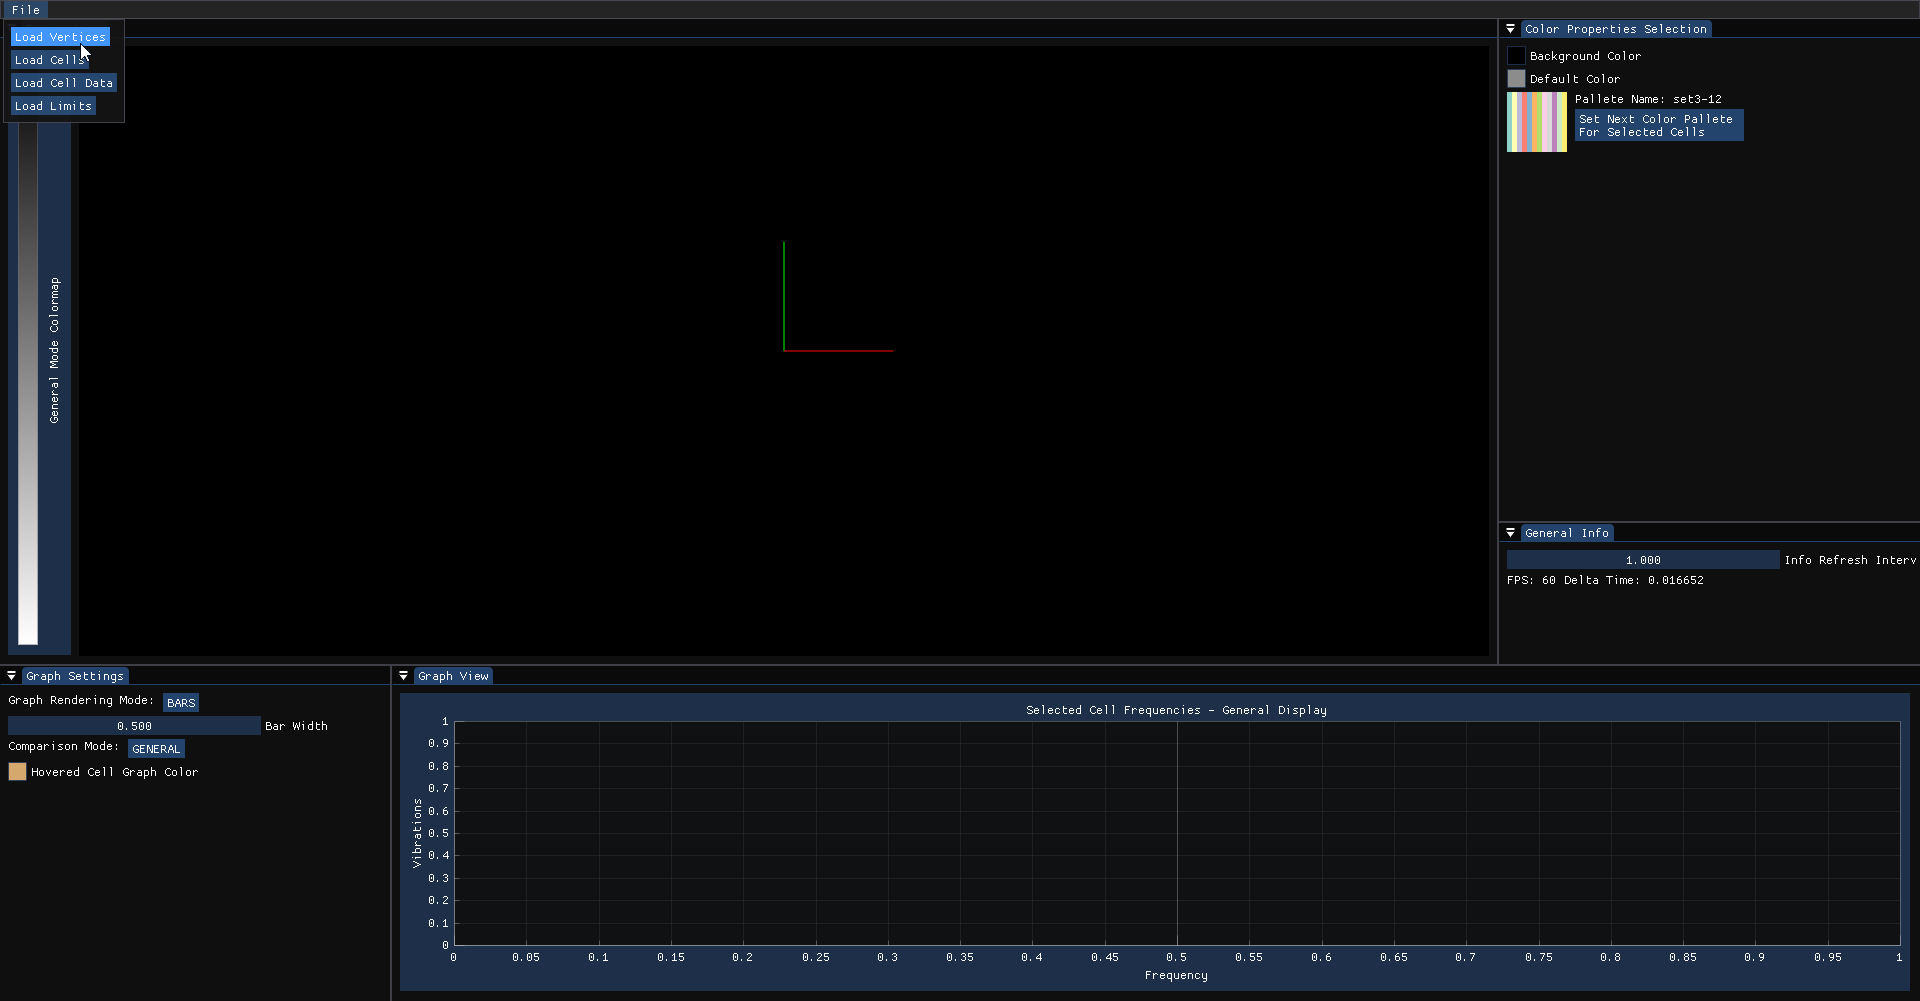
\includegraphics[width=\textwidth]{demonstration/load_file_menu.png}
    \caption{Izbornik za učitavanje datoteka}
    \label{fig:file-menu}
\end{figure}

\begin{figure} [H]
	\centering
    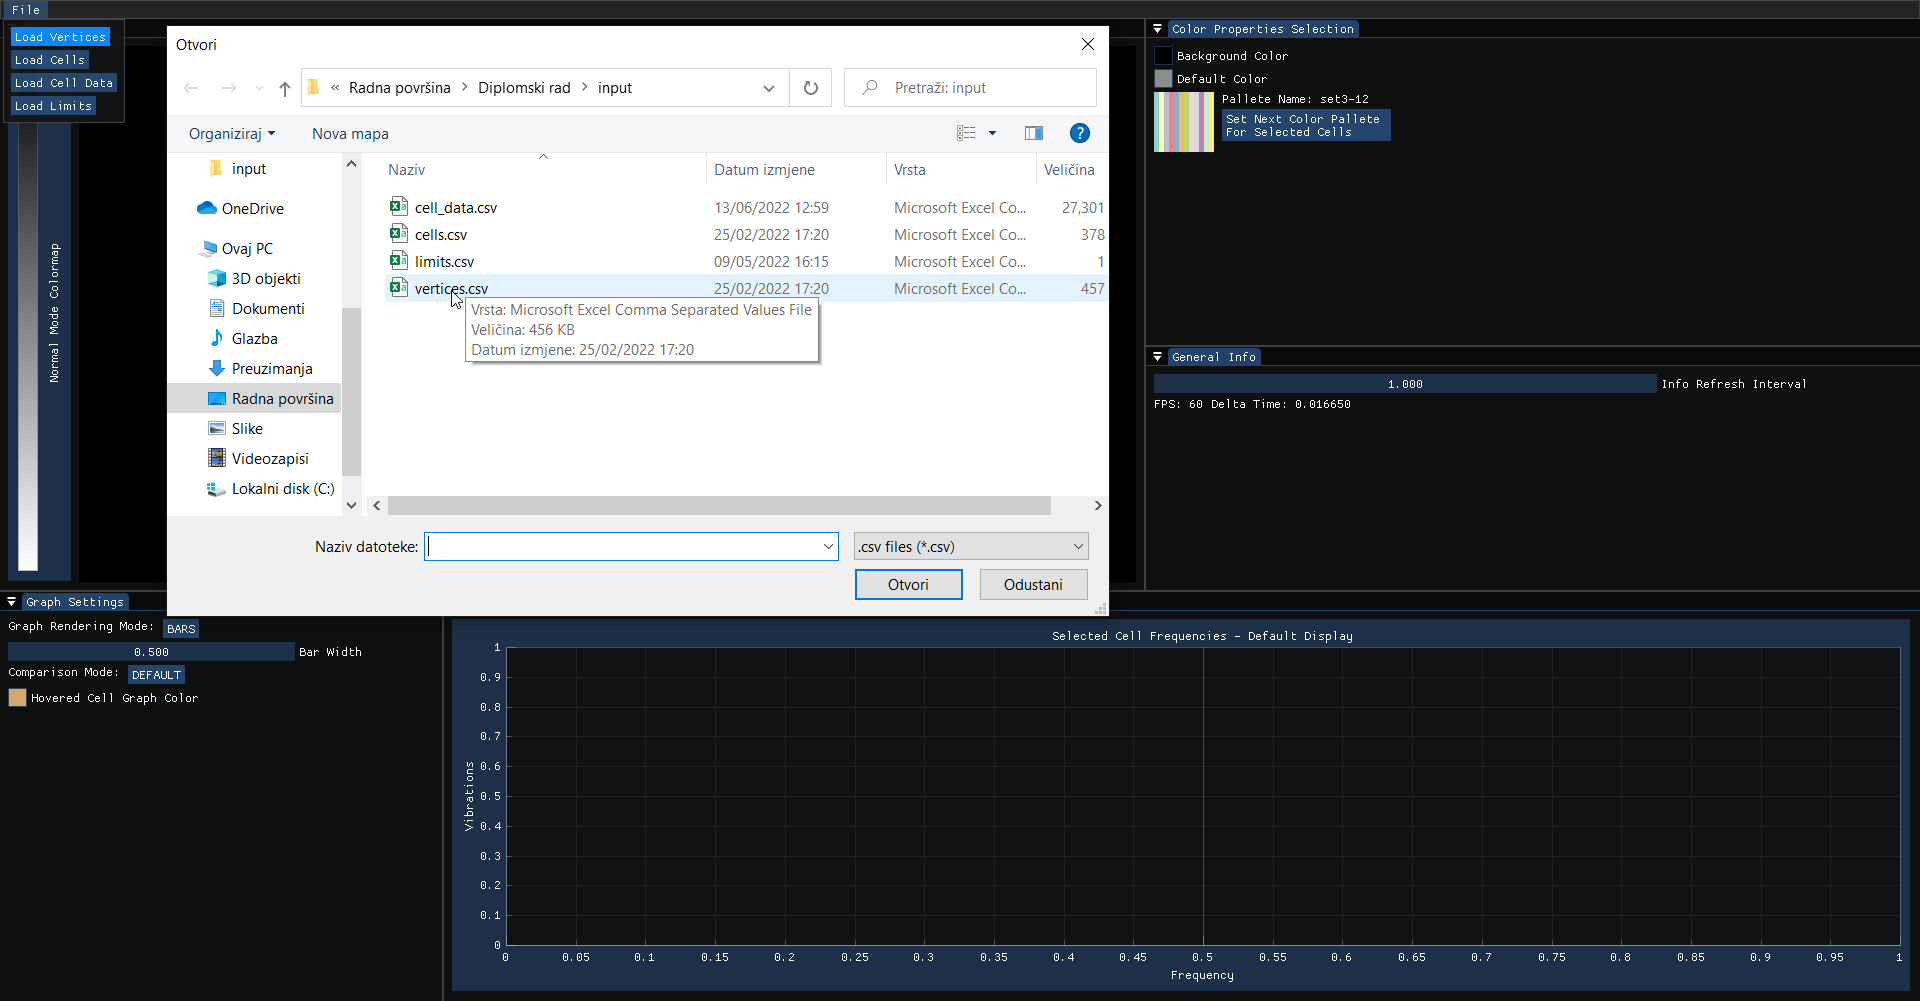
\includegraphics[width=\textwidth]{demonstration/file_select_dialog.png}
    \caption{Dijalog za odabiranje datoteke}
    \label{fig:file-dialog}
\end{figure}

Nakon što su sve moguće datoteke učitane, izgled alata bi trebao sličiti prikazu sa slike \ref{fig:loaded-files-tool}.

\begin{figure} [H]
	\centering
    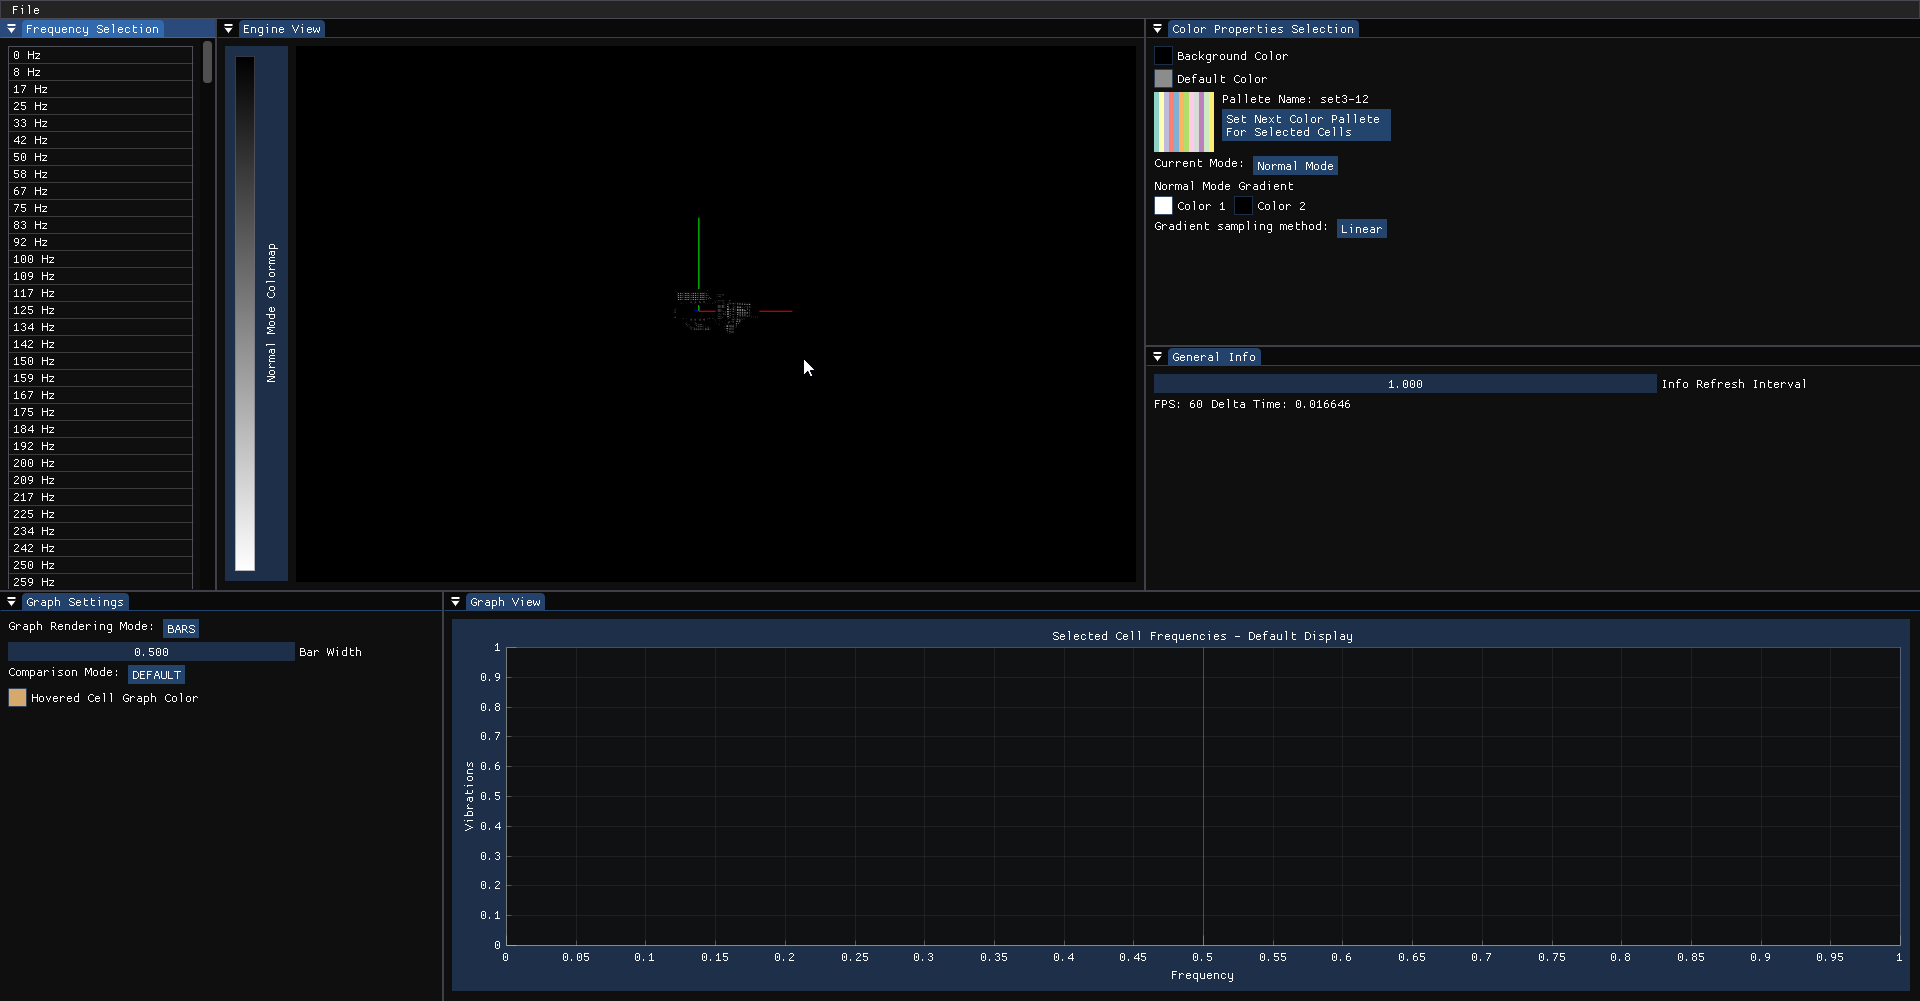
\includegraphics[width=\textwidth]{demonstration/files_loaded_screenshot.png}
    \caption{Prikaz alata nakon što su sve relevantne datoteke učitane}
    \label{fig:loaded-files-tool}
\end{figure}

\section{Normalni način rada}

Alat se u početku uvijek nalazi u normalnom načinu rada. U prikazu alata sa slike \ref{fig:loaded-files-tool} korisnik može odabrati frekvencije vibriranja za koje ga zanima snaga vibracije ćelija motora, na što se boje ćelija motora ažuriraju slično kao na slici \ref{fig:selected-frq}.

\begin{figure} [H]
	\centering
    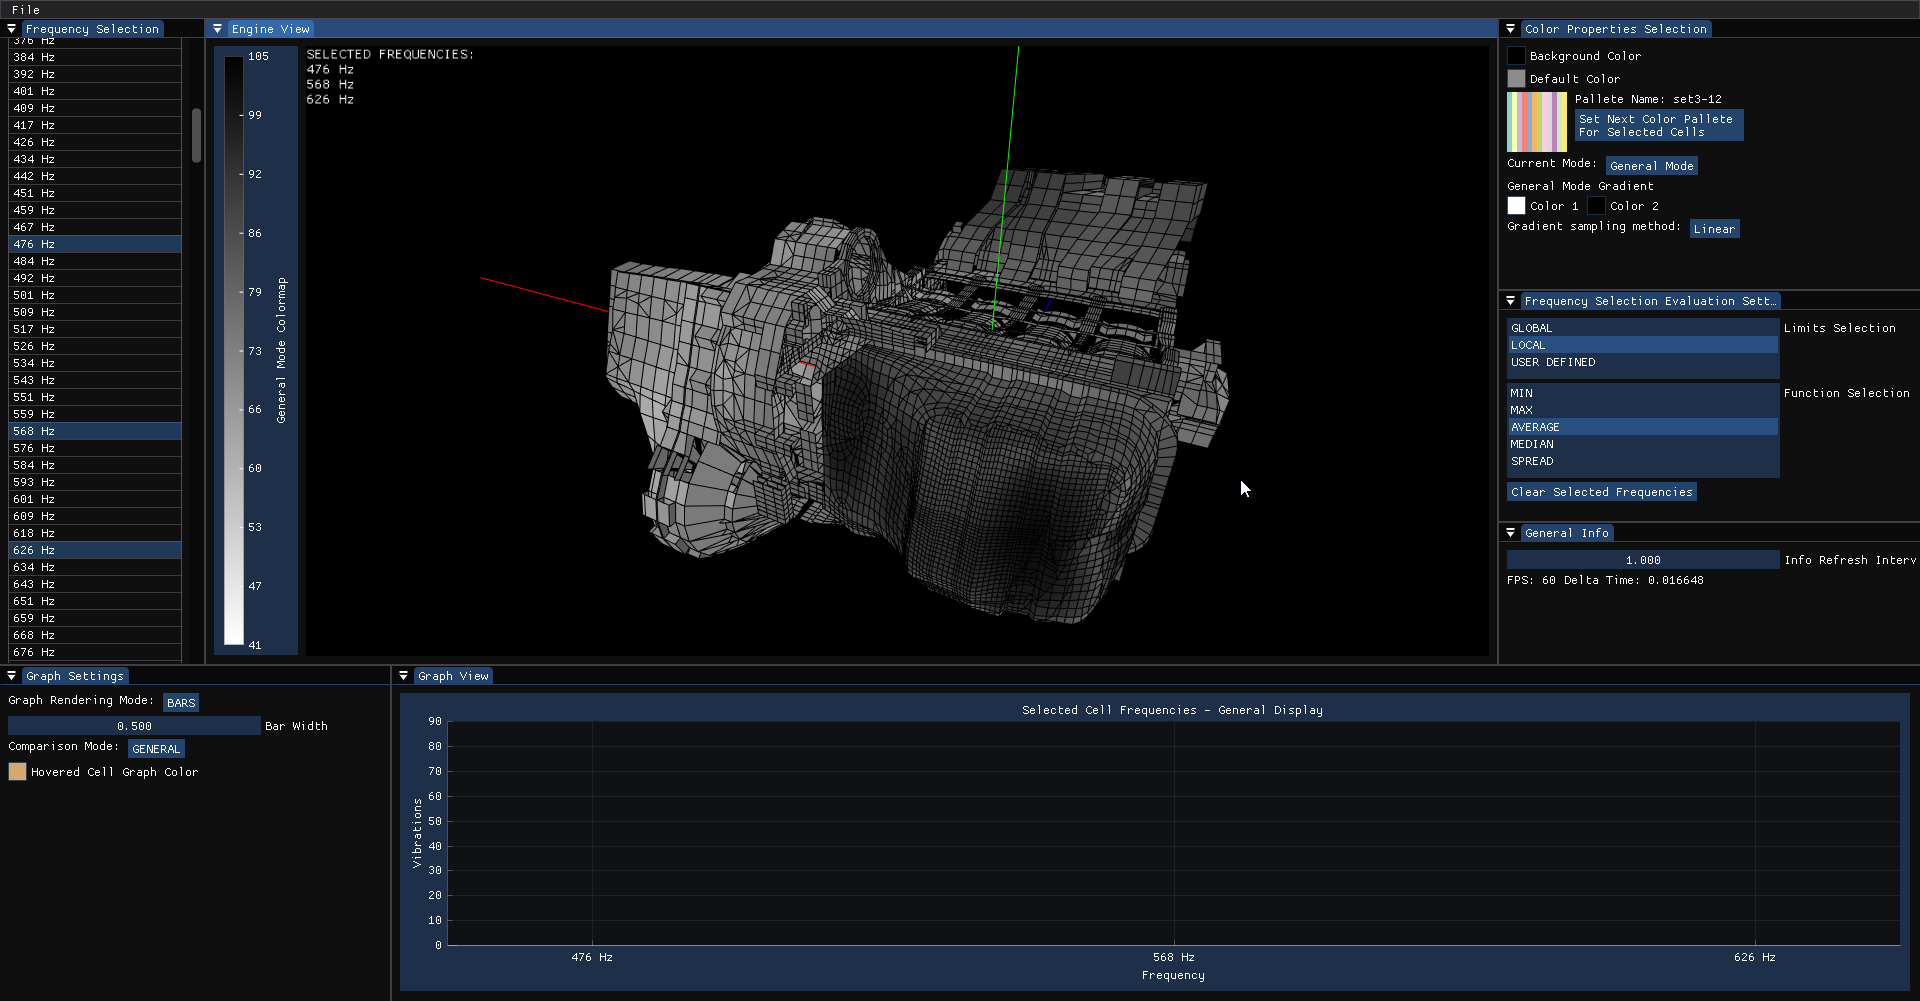
\includegraphics[width=\textwidth]{demonstration/selected_frq.png}
    \caption{Odabiranje frekvencija u normalnom načinu rada alata}
    \label{fig:selected-frq}
\end{figure}

Ako korisniku vidljivost ili izgled početno postavljenog gradijenta ne odgovaraju, moguće je promijeniti boje koje opisuju gradijent, kao što je prikazano na slici \ref{fig:color-select}.

\begin{figure} [H]
	\centering
    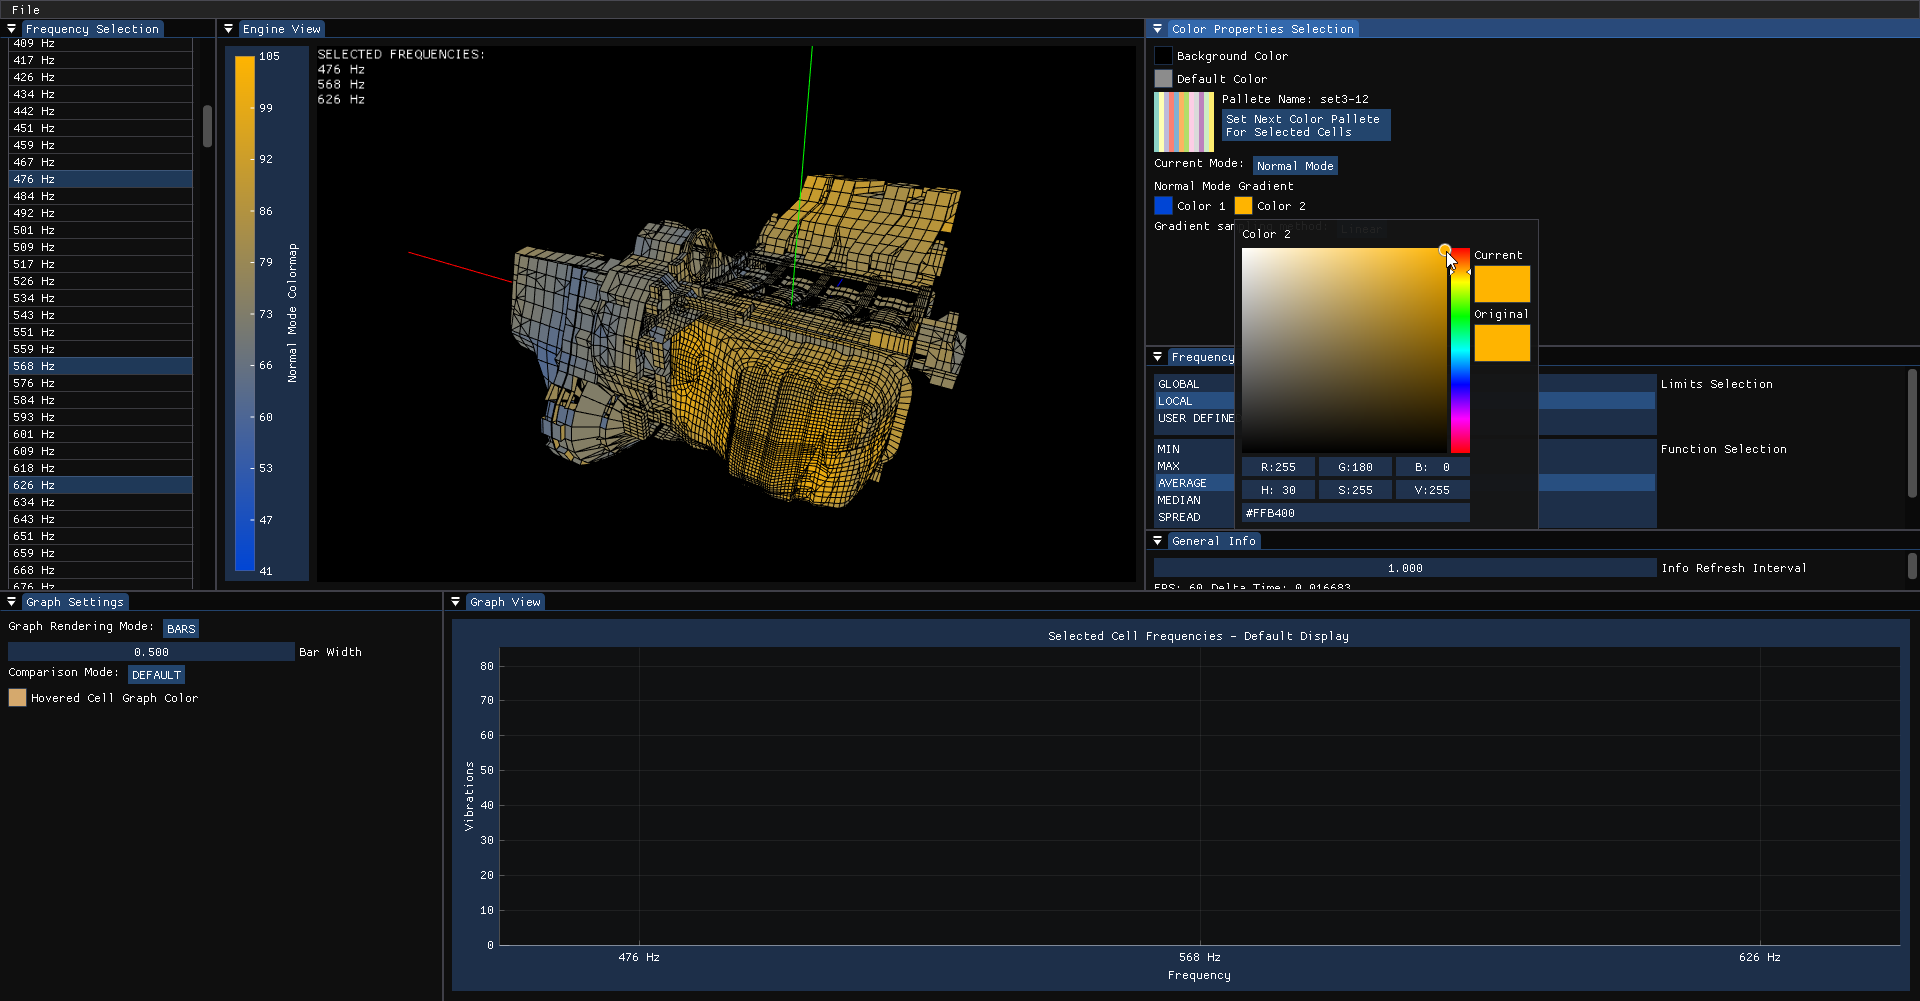
\includegraphics[width=\textwidth]{demonstration/color_select.png}
    \caption{Odabiranje boja gradijenta}
    \label{fig:color-select}
\end{figure}

No, sa slike \ref{fig:color-select} je vidljivo kako boja koja označava vibracije pri vrhu lokalnog raspona zauzima nešto manje od pola gradijenta, što korisniku vjerojatno nije pretjerano korisno ako želi uočiti kritične dijelove motora. Iz tog razloga, korisnik može promijeniti način uzorkovanja gradijenta, a na slici \ref{fig:quartic-engine-colors} se može vidjeti kako kvartičko uzorkovanje uvelike pomaže pri vizualnom izoliranju ekstrema.

\begin{figure} [H]
	\centering
    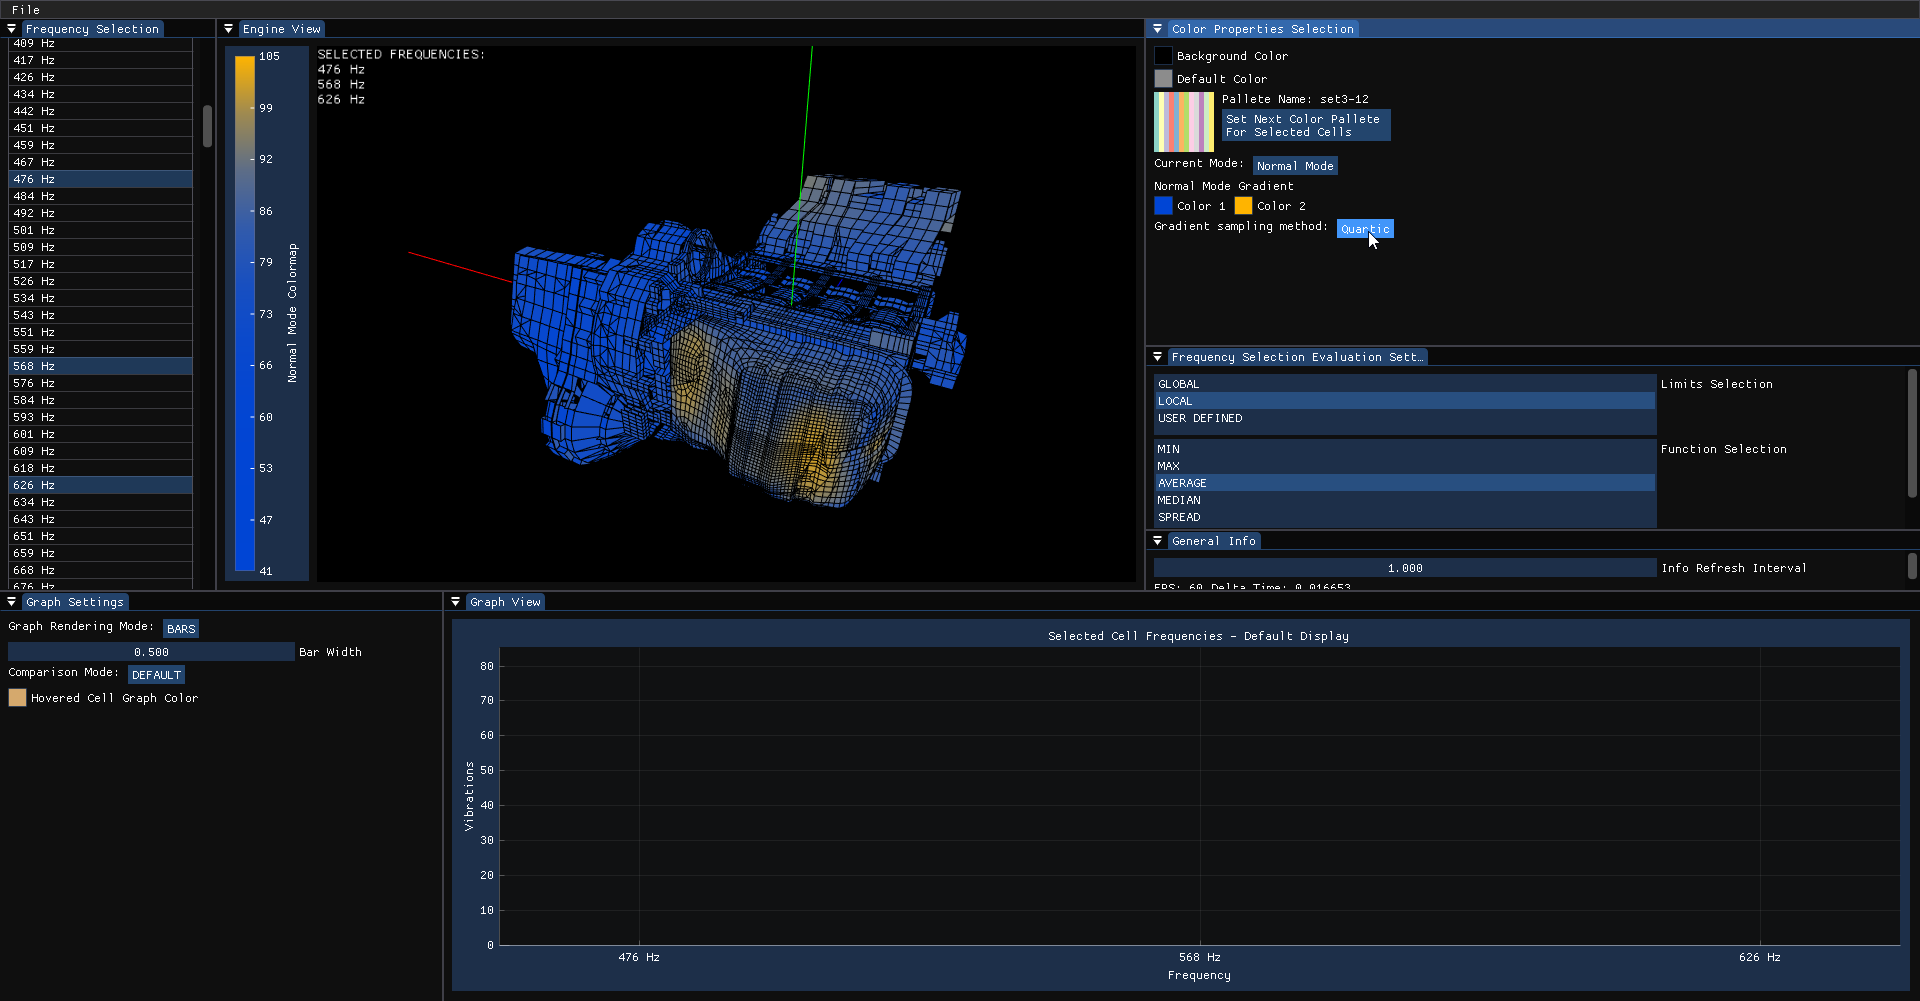
\includegraphics[width=\textwidth]{demonstration/quartic_sampling_normal_mode.png}
    \caption{Boje ćelija motora pri kvartičkom uzorkovanju gradijenta}
    \label{fig:quartic-engine-colors}
\end{figure}

Ako korisnik želi imati veću kontrolu nad isticanjem ekstremnih vrijednosti, može to učiniti "ručnim" definiranjem raspona. Na ovakav način korisnik može definirati proizvoljni minimum i maksimum ekstremnih vrijednosti. No, važno je naglasiti kako je pri ovakvom načinu izoliranja ekstrema dobro koristiti linearno uzorkovanje gradijenta jer ostala uzorkovanja najvjerojatnije neće "kritičnom" bojom obojati većinu ćelija koje pripadaju rasponu ekstremnih vrijednosti kojeg je korisnik definirao. Na slici \ref{fig:custom-interval} se može vidjeti primjer korištenja intervala definiranog od strane korisnika. Na spomenutoj slici se također koristi i funkcija MAX, koja je jako korisna ako korisnika zanima koliko će najjače ćelija vibrirati pri odabranim frekvencijama.

\begin{figure} [H]
	\centering
    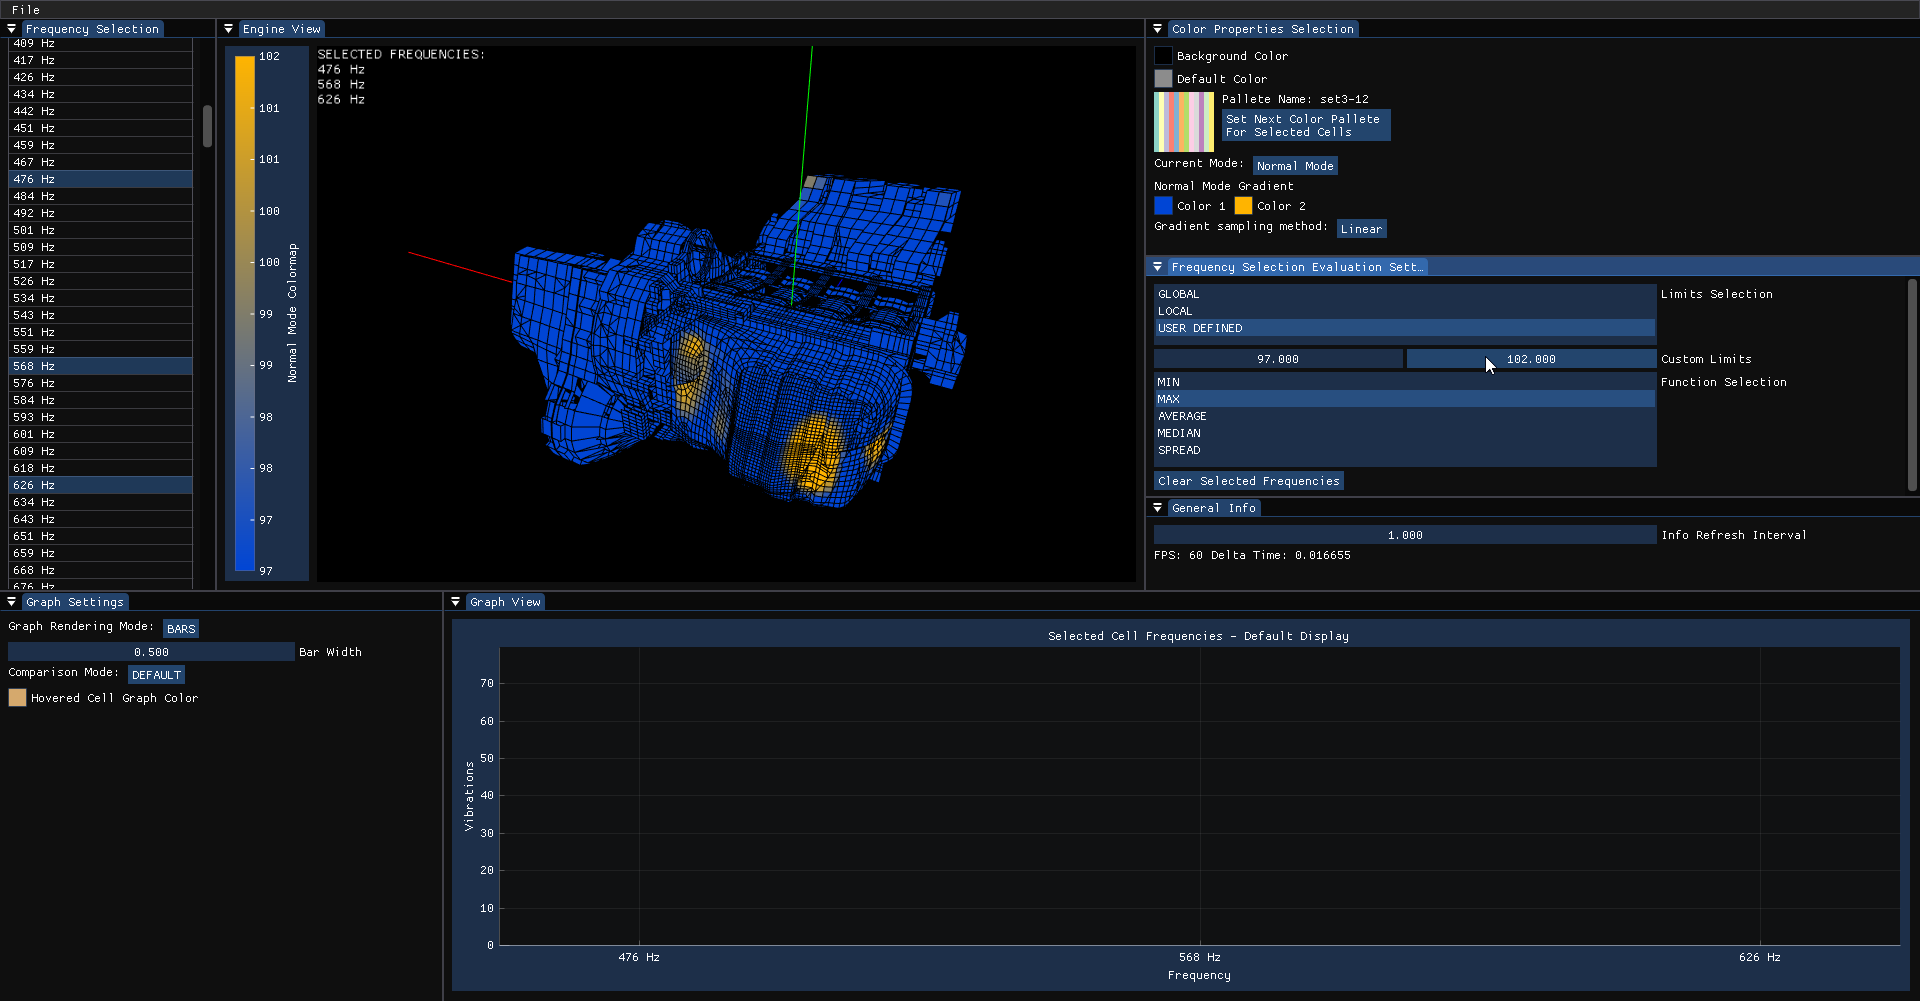
\includegraphics[width=\textwidth]{demonstration/custom_limits_linear_sampling.png}
    \caption{Izgled motora uz "ručno" definirani raspon i korištenje funkcije MAX}
    \label{fig:custom-interval}
\end{figure}

"Ručno" definiranje raspona također može biti korisno i kod korištenja funkcije SPREAD. Izgled motora prilikom korištenja te funkcije je vidljiv na slici \ref{fig:spread-view}. Navedena funkcija vraća razliku između najveće i najmanje snage vibracije ćelije pri odabranim frekvencijama, pa se korištenjem ove funkcije uz raspon definiran od strane korisnika može preciznije definirati koji je raspon razlika u snazi vibriranja ćelija korisniku bitan za uočiti. 

\begin{figure} [H]
	\centering
    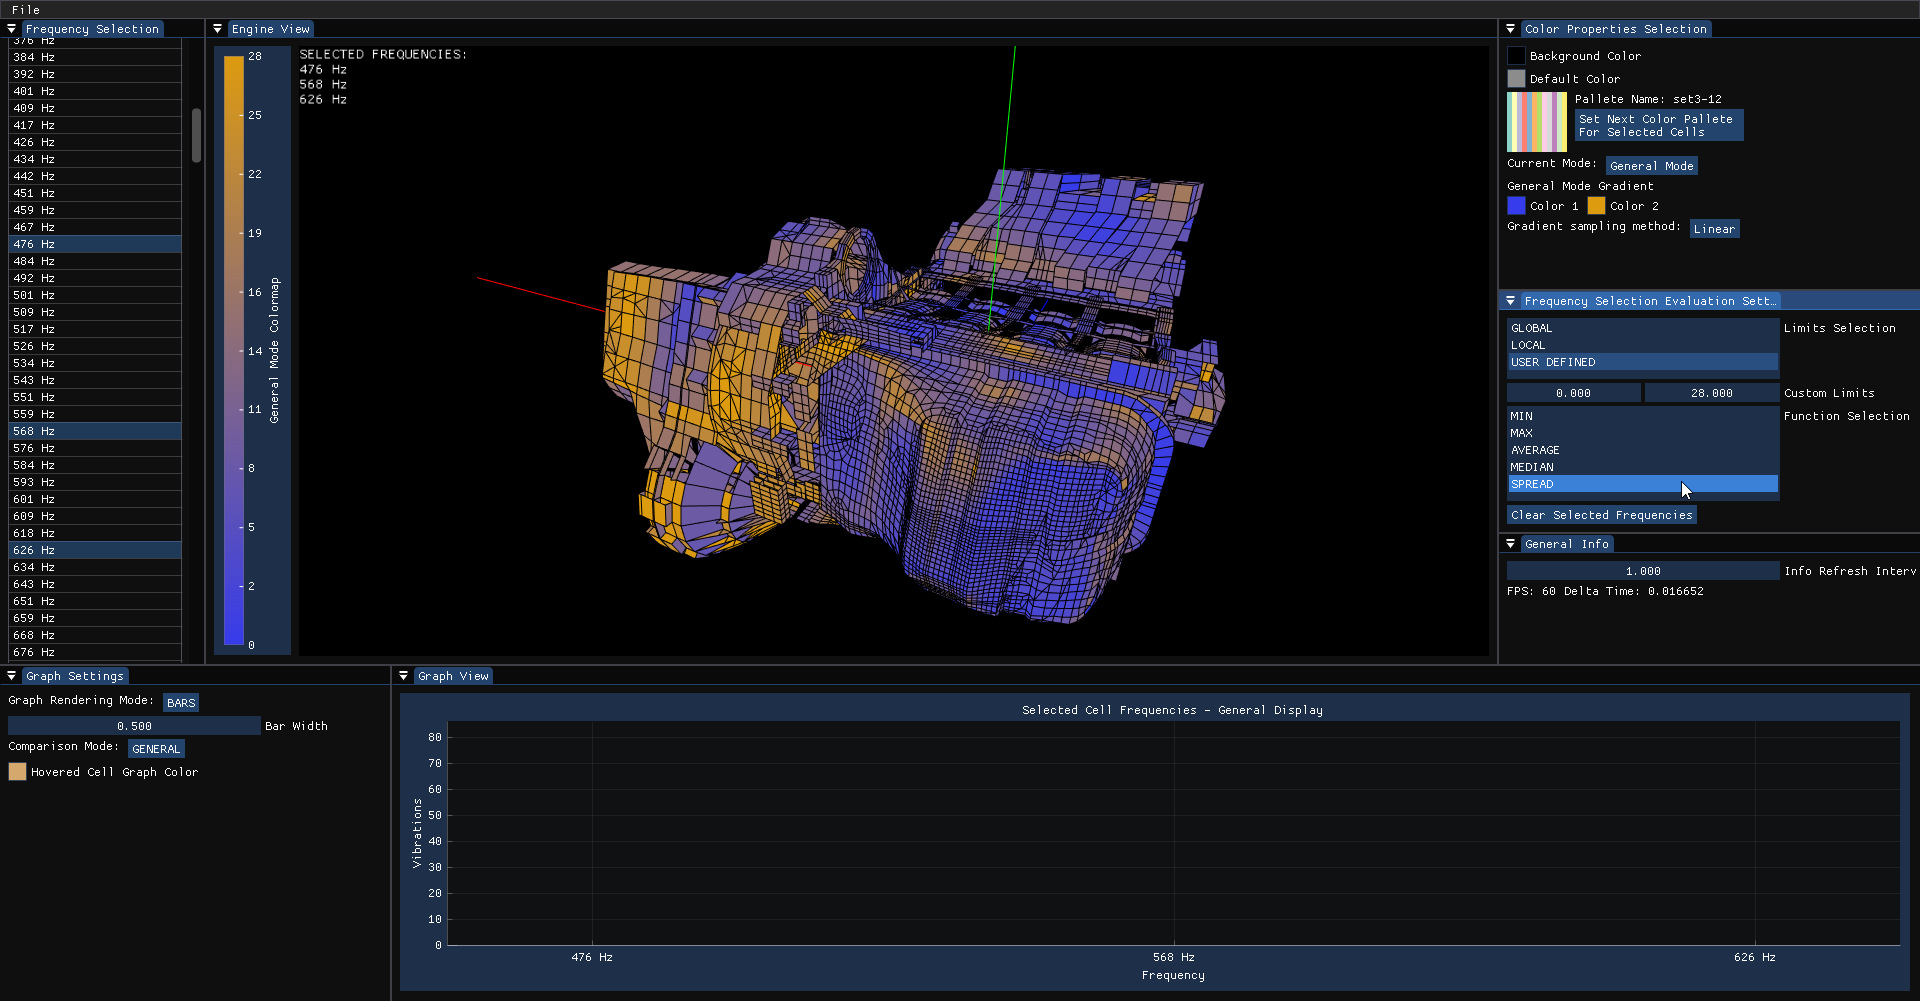
\includegraphics[width=\textwidth]{demonstration/spread.png}
    \caption{Izgled motora pri korištenju funkcije SPREAD uz raspone definirane od strane korisnika}
    \label{fig:spread-view}
\end{figure}

\section{Način rada s preddefiniranim ograničenjima}

Klikom na gumb s imenom trenutnog načina rada alat prelazi iz normalnog načina rada u način rada s preddefiniranim ograničenjima i obratno. Na slici \ref{fig:limits-mode-switched} se može vidjeti kako je broj frekvencija koje se može odabrati u načinu rada s preddefiniranim ograničenjima puno manji nego u normalnom načinu rada jer su samo dostupne frekvencije za koje su ograničenja definirana u datoteci iz koje su učitana.

\begin{figure} [H]
	\centering
    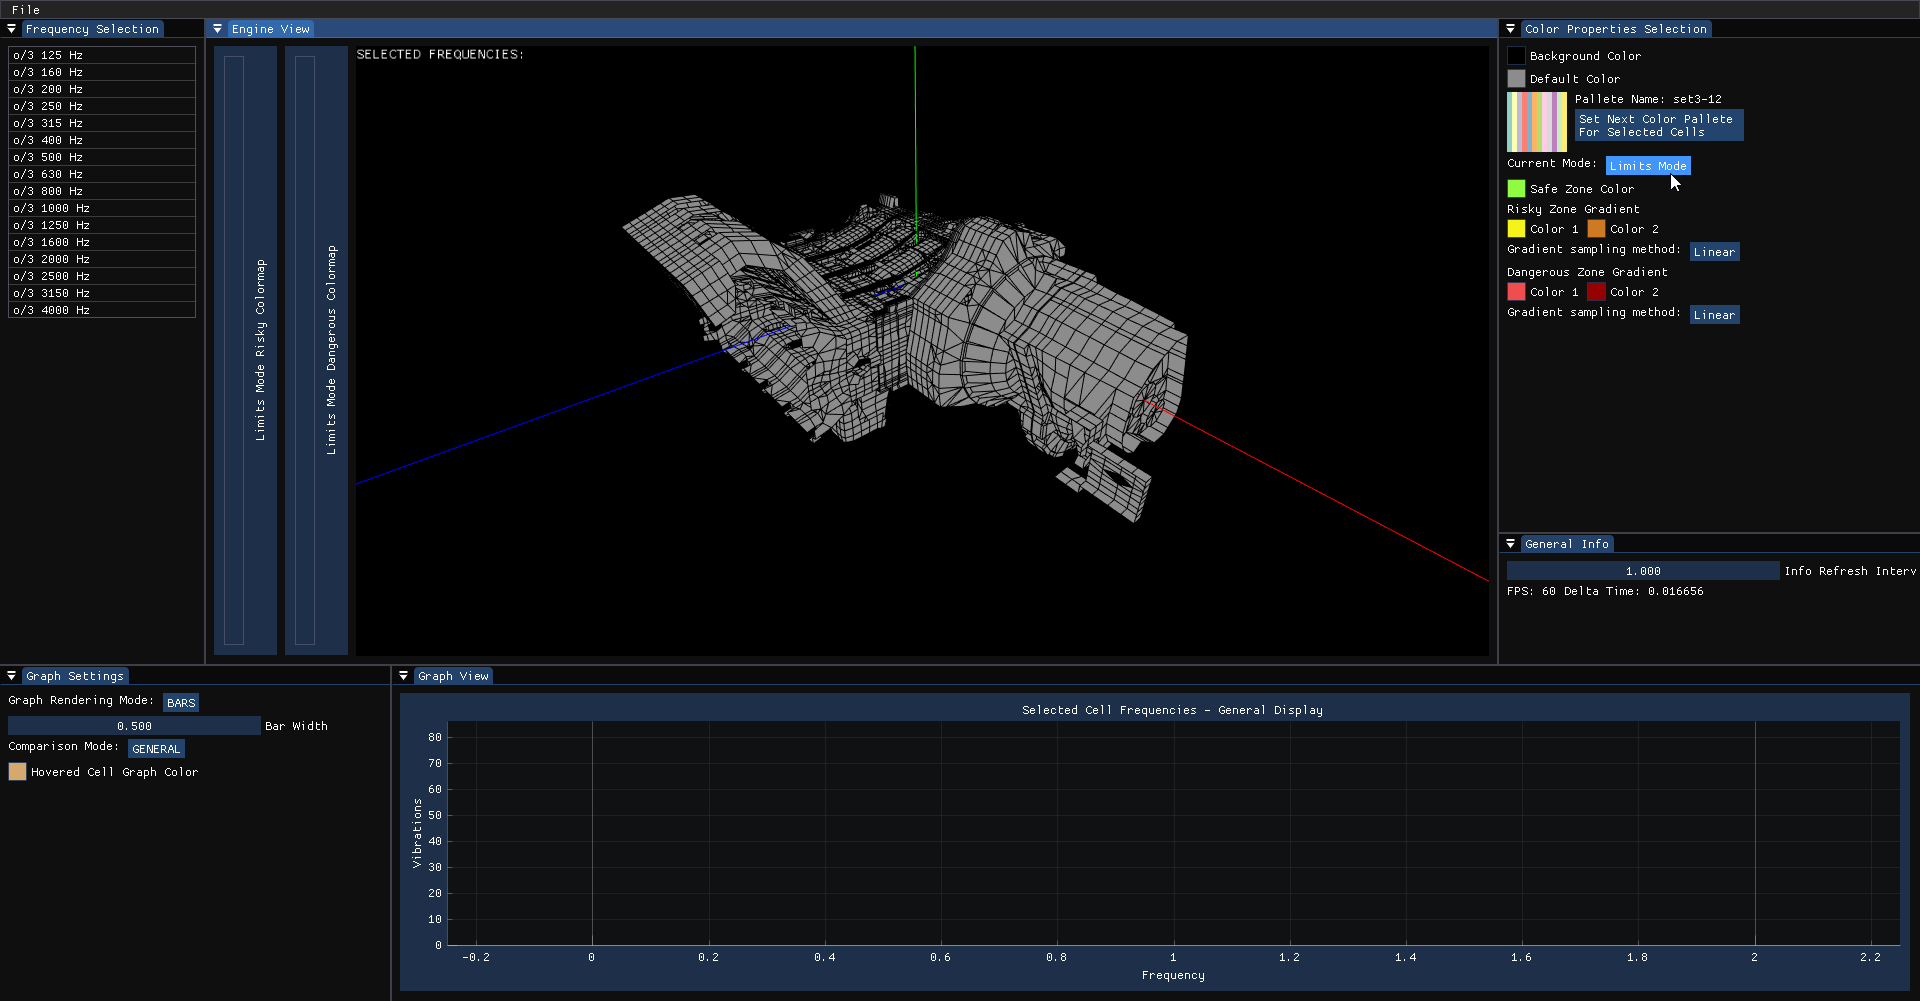
\includegraphics[width=\textwidth]{demonstration/limits_mode_opened.png}
    \caption{Početni izgled alata u načina rada s preddefiniranim ograničenjima}
    \label{fig:limits-mode-switched}
\end{figure}

Na slici \ref{fig:limits-mode-frq-selected} se može vidjeti kako alat izgleda kada je u načinu rada s preddefiniranim ograničenjima odabrano nekoliko ponuđenih frekvencija vibriranja. U ovom načinu rada se također mogu mijenjati boje i metoda uzorkovanja gradijenta.

\begin{figure} [H]
	\centering
    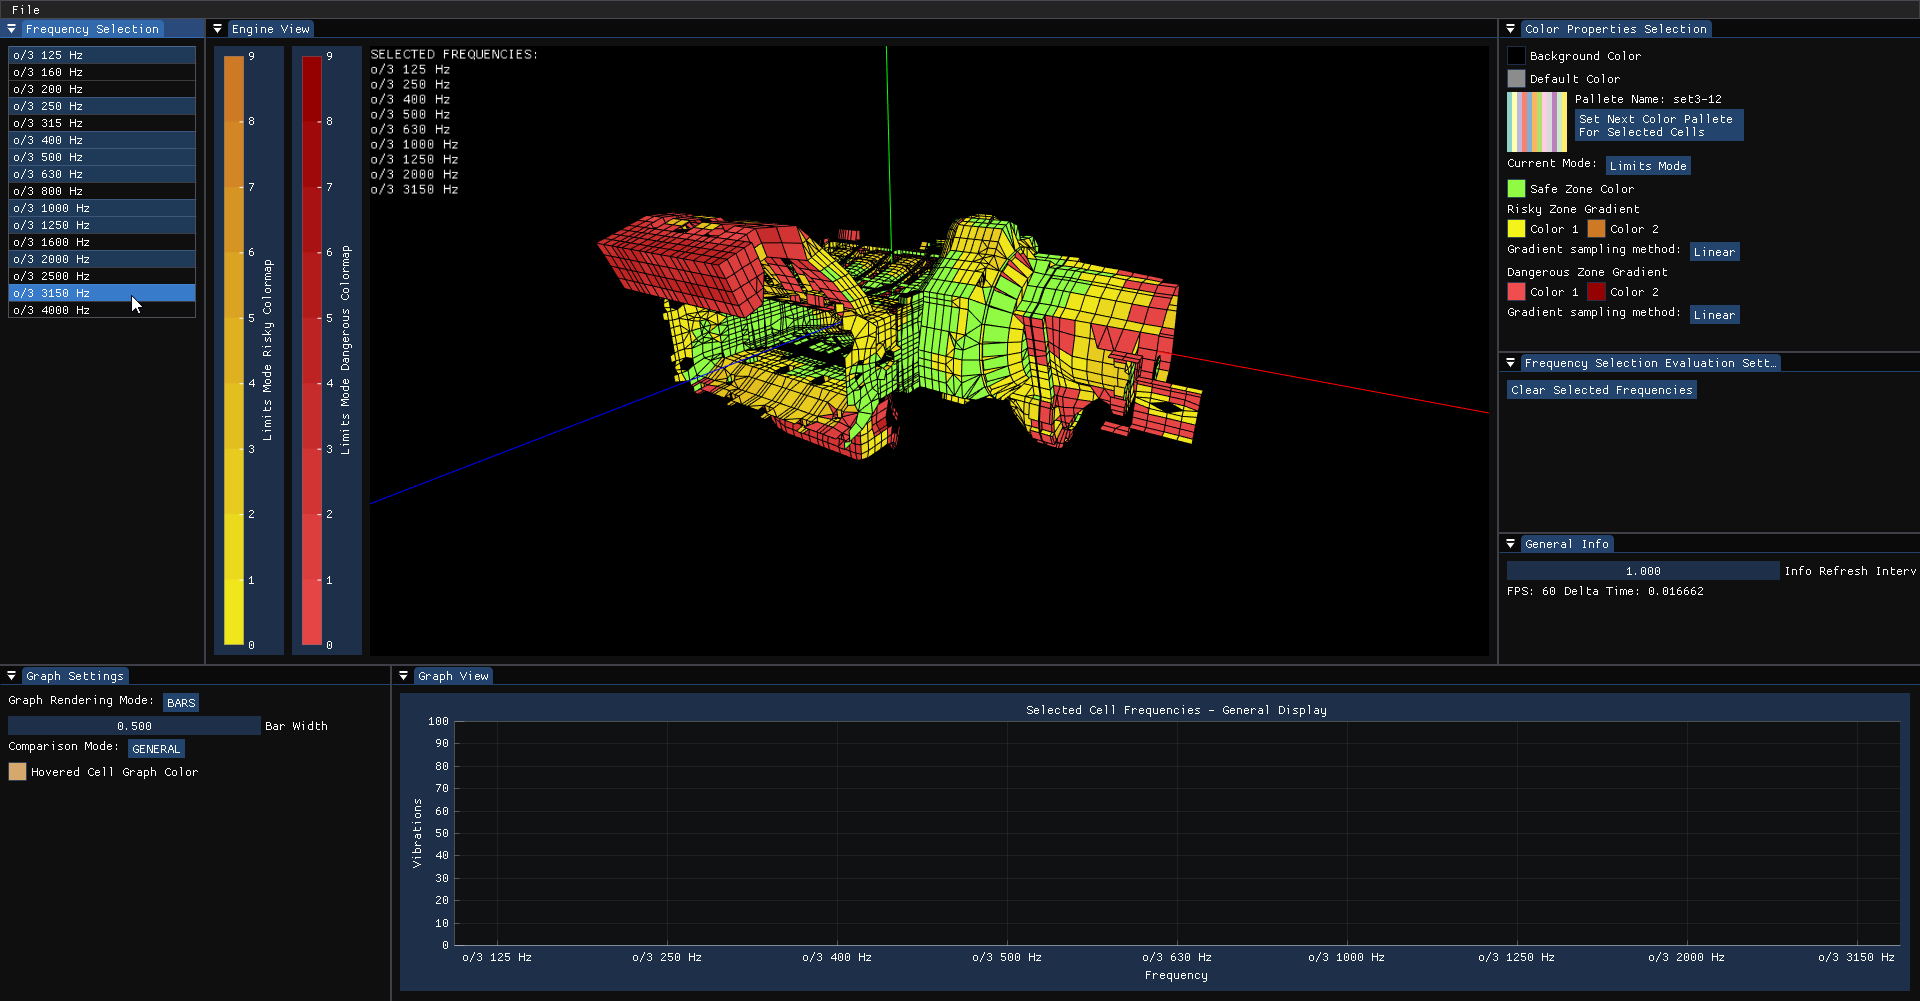
\includegraphics[width=\textwidth]{demonstration/limits_mode_frq_selected.png}
    \caption{Nekoliko odabranih frekvencija u načinu rada s preddefiniranim ograničenjima}
    \label{fig:limits-mode-frq-selected}
\end{figure}

\section{Uspoređivanje ćelija pomoću grafova}

Boje ćelija motora daju samo grubi pregled snage vibracije ćelija, ali ako korisnik želi detaljno analizirati kako se snaga vibracije ćelije mijenja s obzirom na odabrane frekvencije, može koristiti 2D grafove koje alat nudi. Na slici \ref{fig:hovered-graph} se može vidjeti kako alat iscrtava 2D graf ćelije iznad koje korisnik postavi pokazivač miša, a u tom grafu su prikazani podaci o snazi vibracije interesne ćelije pri svim odabranim frekvencijama. Kao što je u prijašnjim poglavljima već spomenuto, navedena ćelija se naziva "lebdeća" ćelija, a boja grafa navedene ćelije se može mijenjati u postavkama grafa, koje se na spomenutoj slici nalaze u donjem lijevom kutu alata.

\begin{figure} [H]
	\centering
    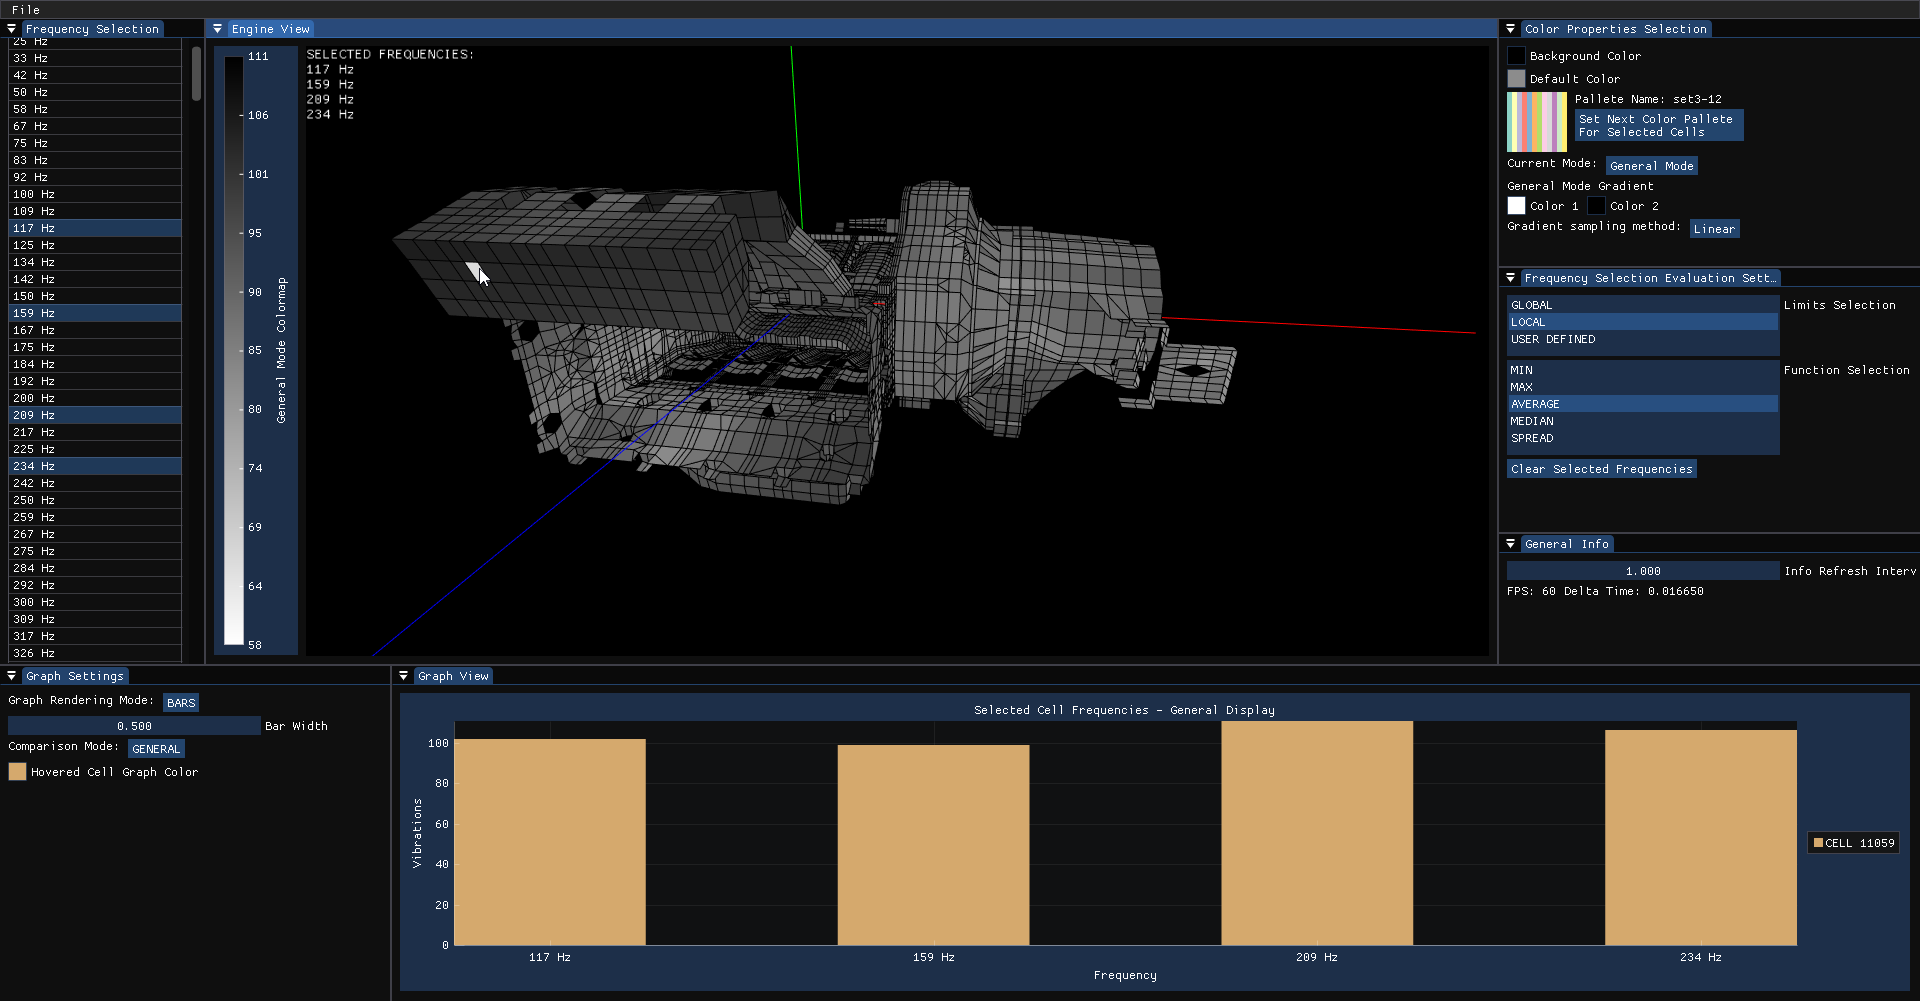
\includegraphics[width=\textwidth]{demonstration/cell_hovered.png}
    \caption{Graf "lebdeće" ćelije}
    \label{fig:hovered-graph}
\end{figure}

Korisnik trenutnu "lebdeću" ćeliju može dodati u listu odabranih ćelija klikom na lijevu tipku miša, ali ako je "lebdeća" ćelija već u listi odabranih ćelija, lijevi klik miša će tu ćeliju maknuti iz liste. Odabiranjem ćelija, korisnik može detaljnije uspoređivati njihovu snagu vibracije s obzirom na odabrane frekvencije. Kao što je vidljivo sa slike \ref{fig:selected-cells-graphs}, odabrane ćelije su obojane bojom iz trenutne palete, a grafovi im se konstantno nalaze u prikazu grafova. 

\begin{figure} [H]
	\centering
    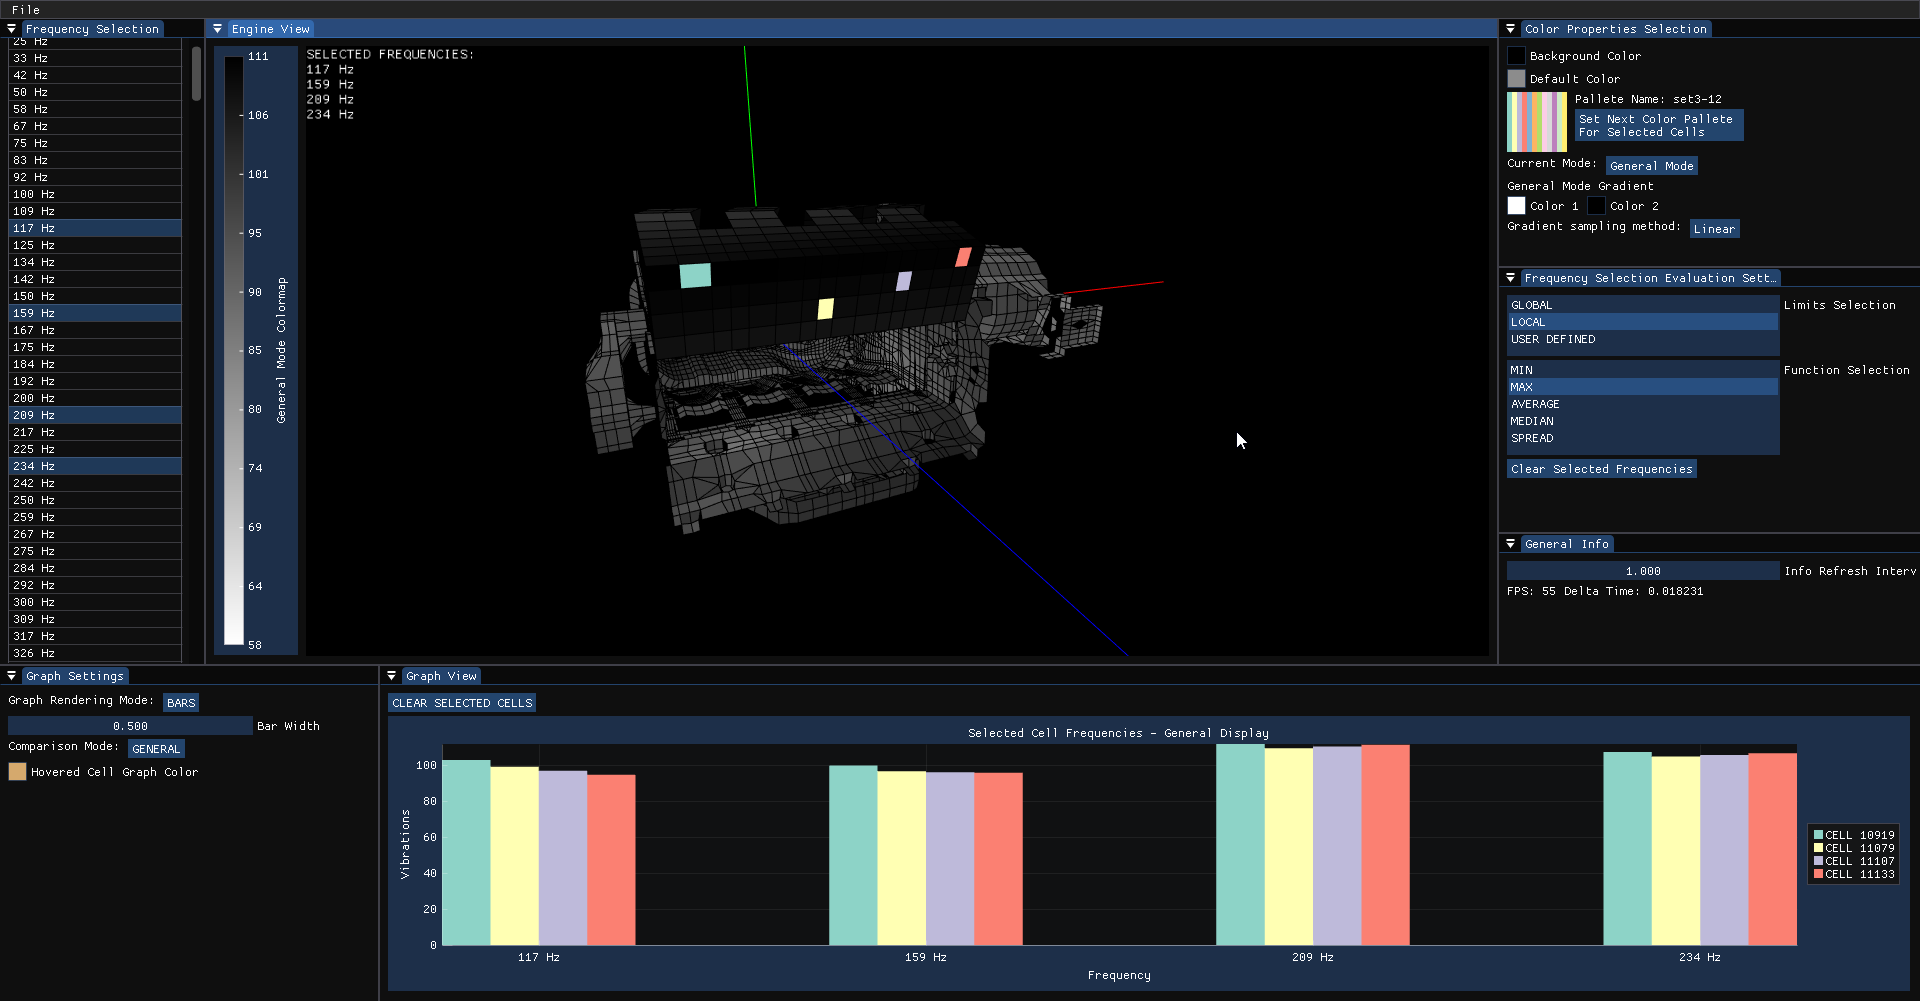
\includegraphics[width=\textwidth]{demonstration/selected_cells_max.png}
    \caption{Usporedba grafova odabranih ćelija}
    \label{fig:selected-cells-graphs}
\end{figure}

Važnost grafova pri uspoređivanju vibracija ćelija postaje očitija ako se usporede slike \ref{fig:selected-cells-graphs} i \ref{fig:hovered-cell-selected-cells} jer promatrajući dijelove motora prikazane na tim slikama, je vidljivo kako su ćelije na ta dva dijela motora slično obojane. Tek kada korisnik postavi pokazivač miša iznad jedne od ćelija sa slike \ref{fig:hovered-cell-selected-cells} postane očito kako se ćelije ne ponašaju ni približno slično.

\begin{figure} [H]
	\centering
    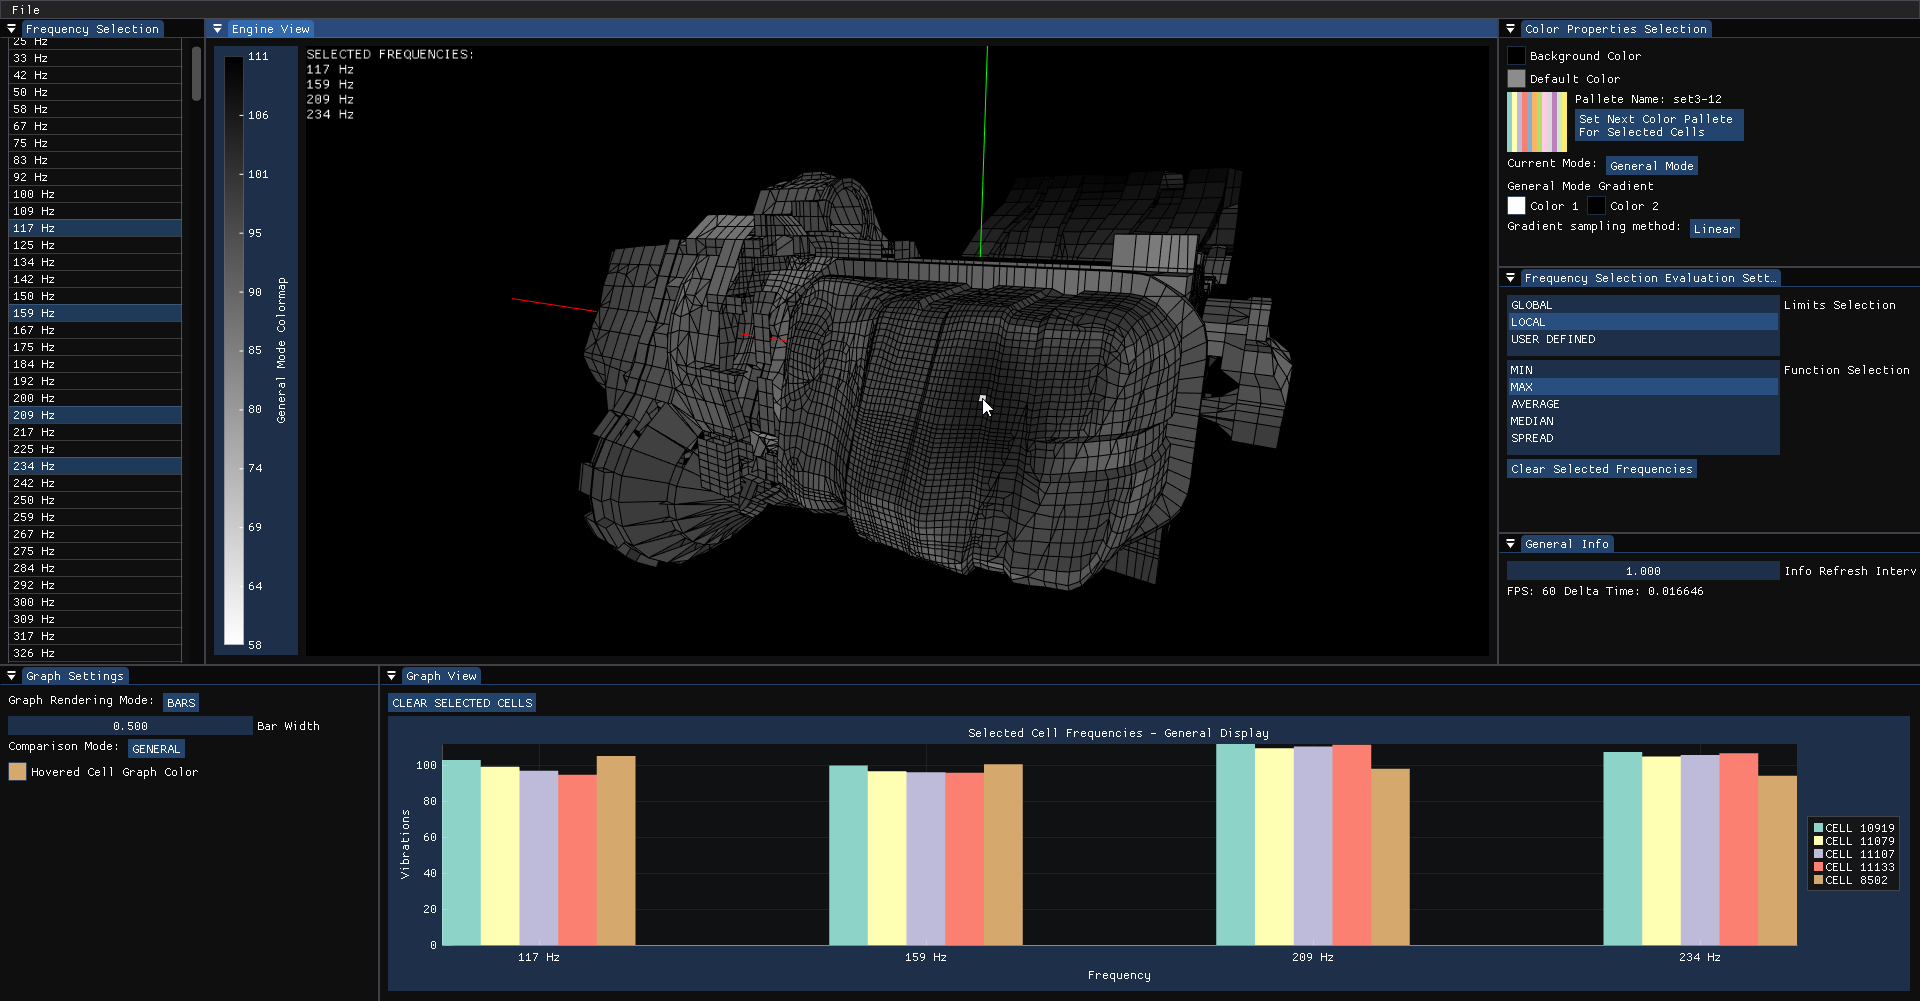
\includegraphics[width=\textwidth]{demonstration/hovered_cell_max.png}
    \caption{"Lebdeća" ćelija koja ima približan maksimum kao i odabrane ćelije na drugom dijelu motora}
    \label{fig:hovered-cell-selected-cells}
\end{figure}

Korisnik može promijeniti način usporedbe klikom na gumb koji nosi ime trenutnog načina usporedbe (u postavkama grafa). Slike \ref{fig:subplots-graph-comp} i \ref{fig:relative-graph-comp} prikazuju dodatne moguće načine na koje korisnik može usporediti odabrane ćelije.


\begin{figure} [H]
	\centering
    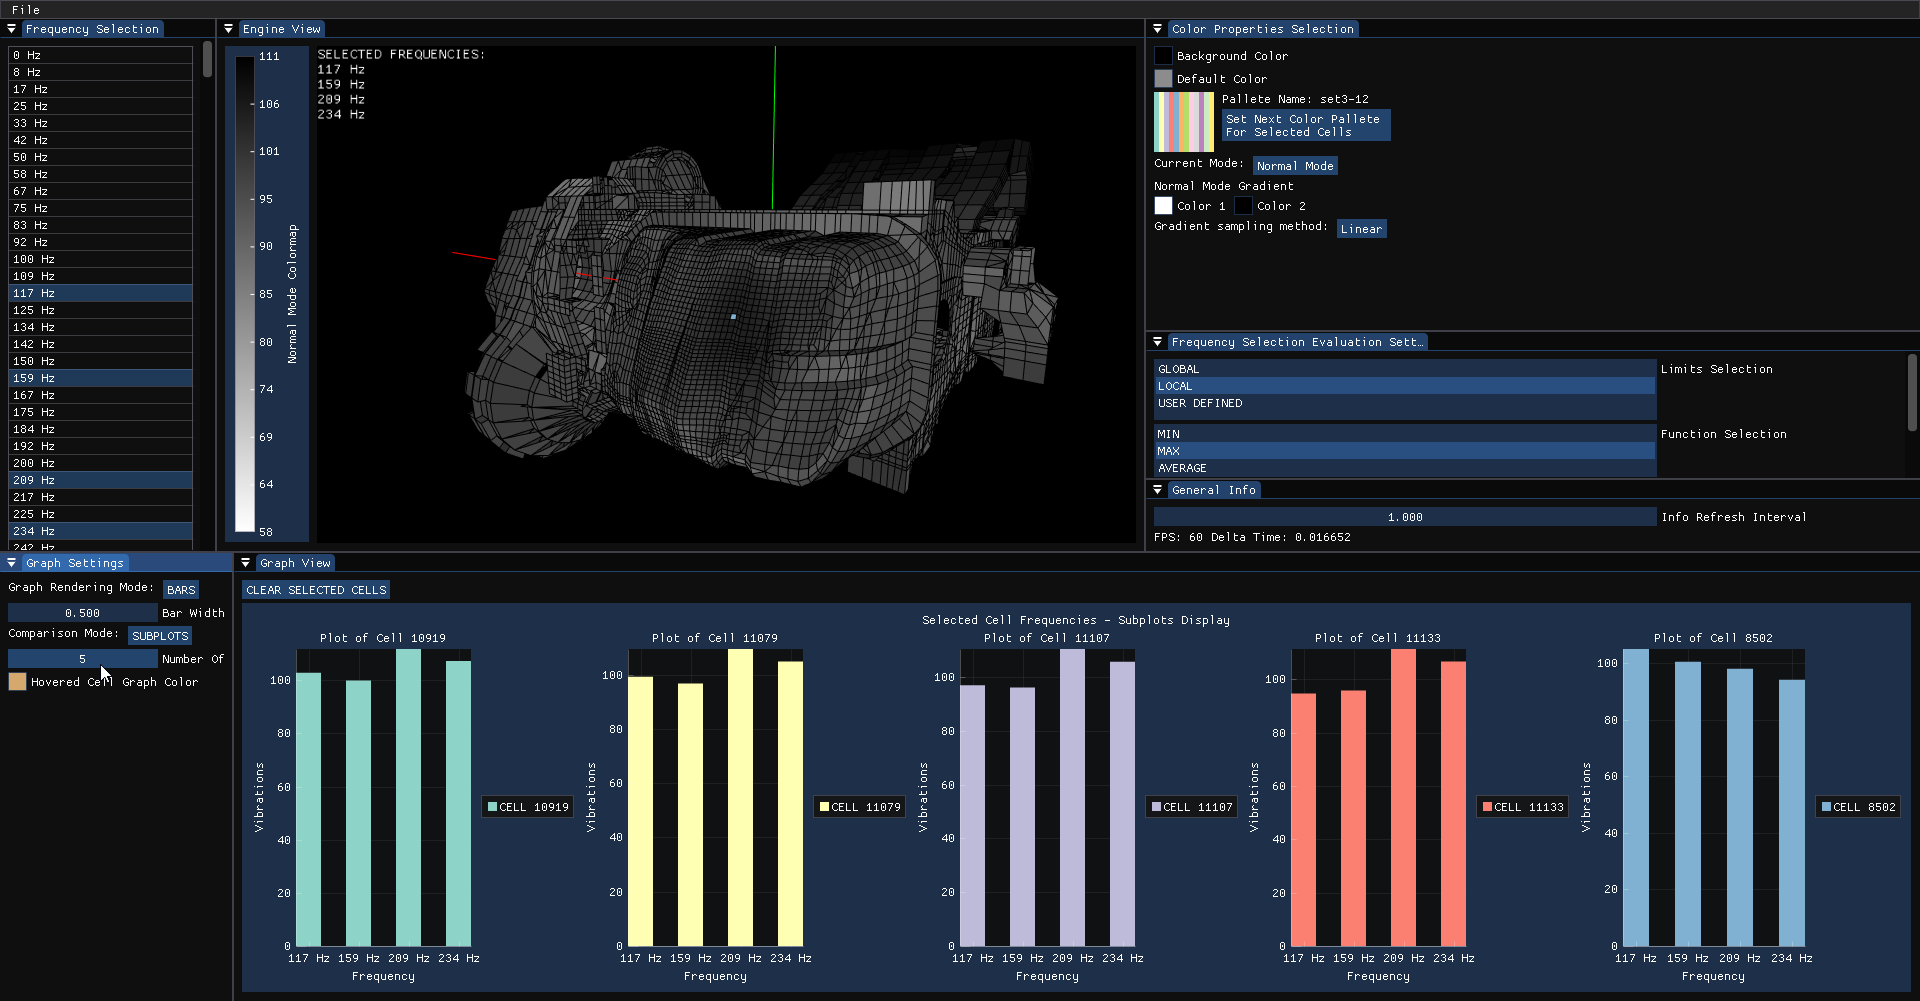
\includegraphics[width=\textwidth]{demonstration/selected_cell_subplots.png}
    \caption{Prikaz grafova u načinu usporedbe s višestrukim prikazima}
    \label{fig:subplots-graph-comp}
\end{figure}

\begin{figure} [H]
	\centering
    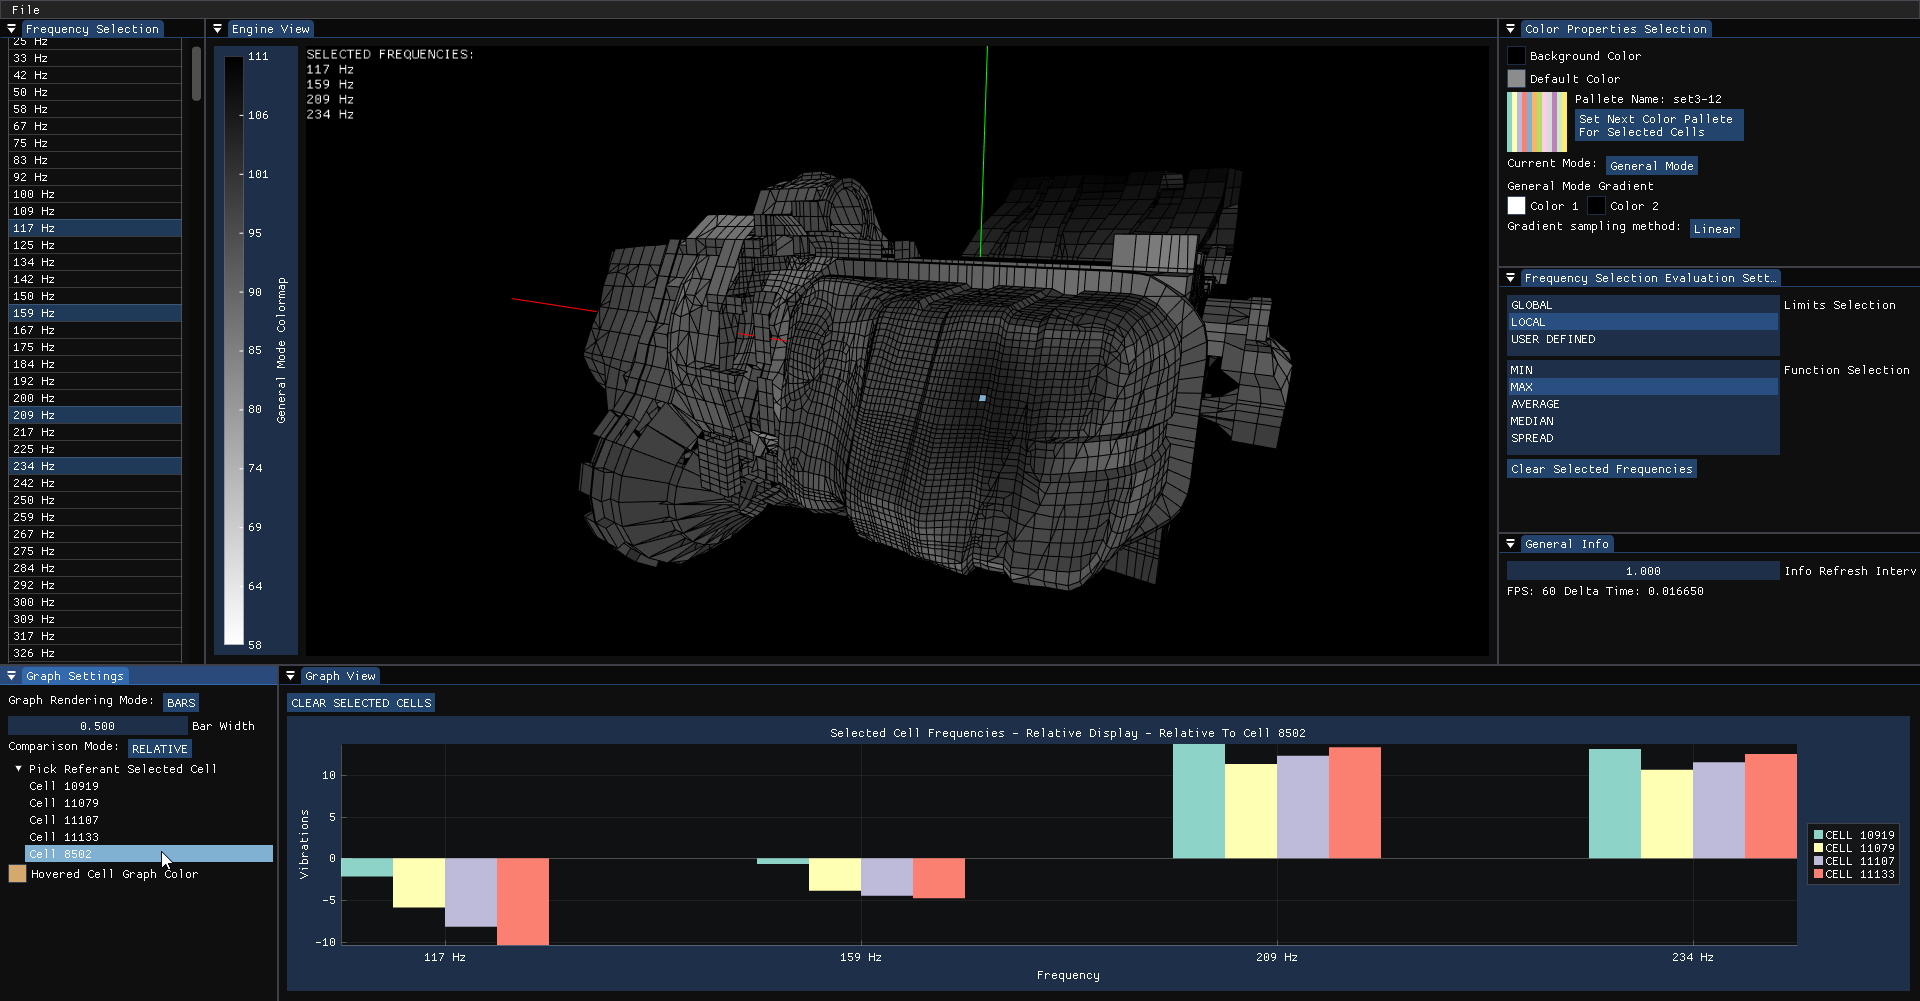
\includegraphics[width=\textwidth]{demonstration/selected_cell_relative.png}
    \caption{Prikaz grafova u relativnom načinu usporedbe}
    \label{fig:relative-graph-comp}
\end{figure}

\chapter{Zaključak}

Alat razvijen u sklopu ovog rada uvelike poboljšava mogućnosti uspoređivanja snaga vibracija dijelova motora na različitim frekvencijama vibriranja. U sklopu alata se korisniku nude dva načina rada koji različito prikazuju iste podatke na modelu motora. Normalni način rada omogućuje odabir više frekvencija na temelju kojih će se određivati boje dijelova motora, ali omogućuje i odabir funkcije pomoću koje će se niz podataka o snazi vibracije dijelova motora na odabranim frekvencijama evaluirati u konačni podatak. Način rada s preddefiniranim ograničenjima korisniku pruža mogućnost definiranja ograničenja na temelju kojih će se ćelije motora svrstati u tri klase s obzirom na snagu vibriranja na odabranim frekvencijama vibracije motora. Osim vizualizacije podataka pomoću 3D modela motora, alat prikazuje podatke korisniku i pomoću 2D grafova za koje su implementirana tri načina uspoređivanja. Spomenuti grafovi nisu zamjena za prikaz podataka na modelu motora, već su nadopuna jer korisniku pružaju mogućnost detaljnije i preciznije analize podataka vezanih za odabrane frekvencije i ćelije.\\

Za alat bi bilo dobro kad bi se nastavio razvijati u smjeru pokrivanja funkcionalnosti iz rada \citep{matkovic2021getting}, prvenstveno dodataka poput interaktivne selekcije i vezanih višestrukih prikaza jer bi navedeni dodaci uvelike doprinijeli jednostavnosti korištenja alata. Ručno spremanje postavki alata bi također bilo koristan dodatkak, s time da bi te postavke uključivale ne samo raspored prozora, već i odabrane gradijente, boje i ostale faktore koje korisnik može mijenjati u alatu. No, na kraju bi najvažnije bilo dodatno evaluirati alat u suradnji sa stručnjacima koji bi ga koristili, kako bi se dobile povratne informacije o unaprjeđivanju postojećih i implementaciji novih mogućnosti koje bi stručnjacima bile od velike koristi.

\bibliography{literatura}
\bibliographystyle{fer}

\appendix
\chapter{Različiti načini crtanja grafova} \label{appendix:graph-display-examples}

\begin{figure}[H]
	\centering
	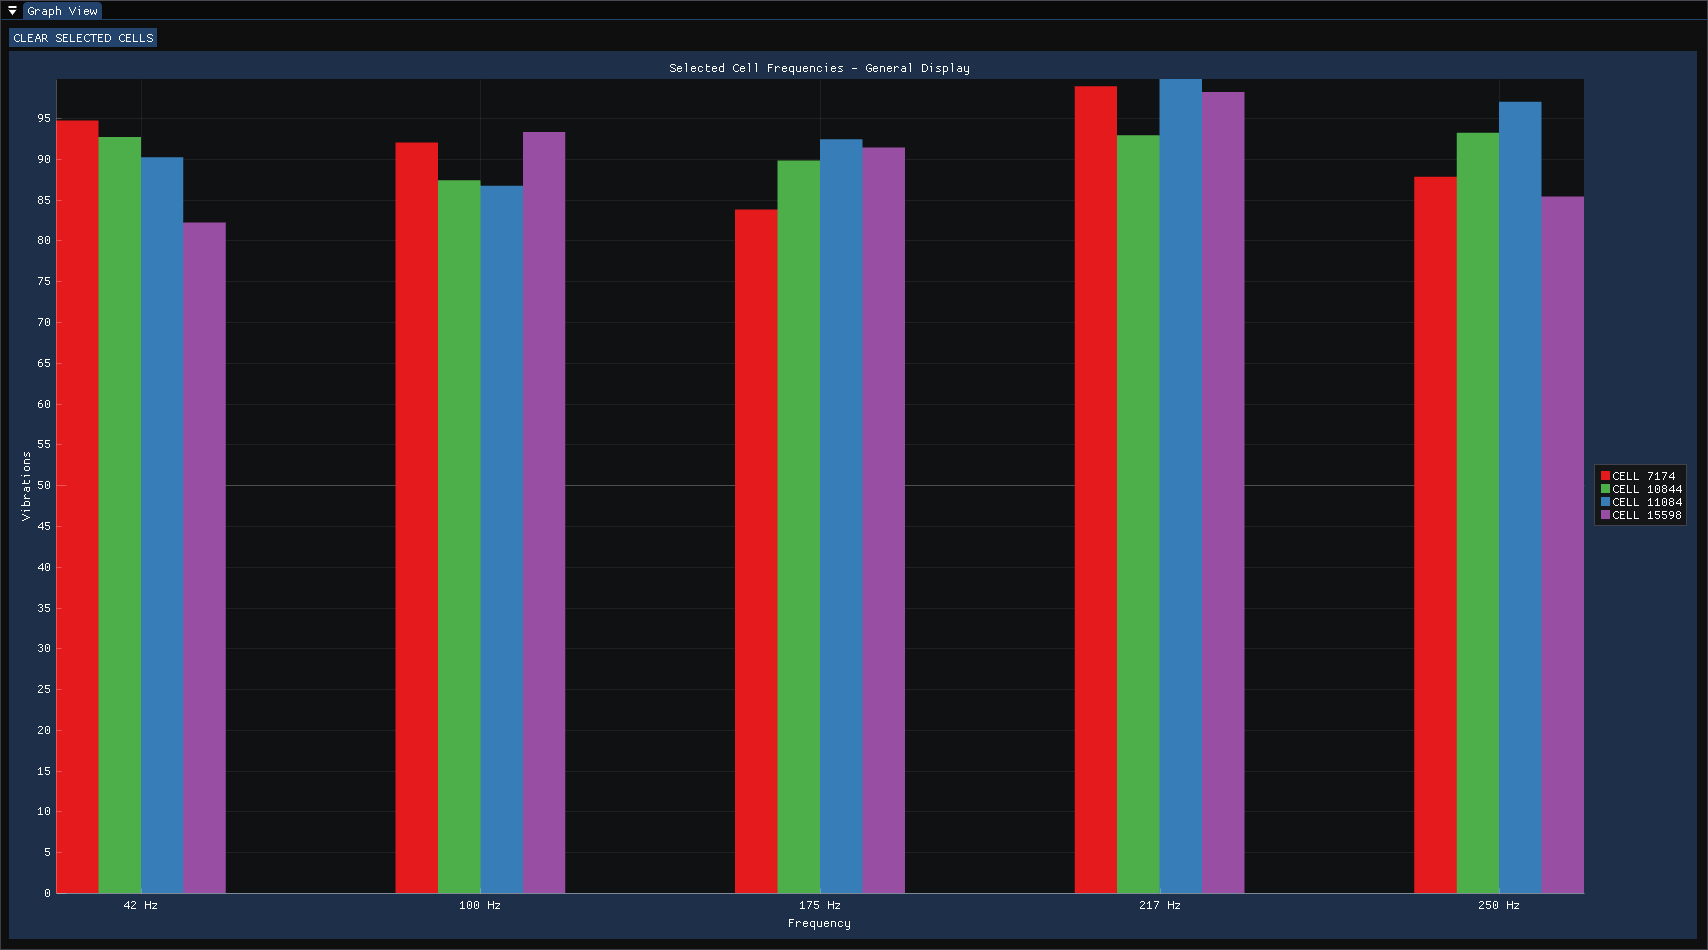
\includegraphics[width=\textwidth]{default_graph_display_bars.png}
	\caption{Normalni način usporedbe grafova u obliku stupaca}
    \label{appendix:default_graph_display_bars}
\end{figure}

\begin{figure}[H]
	\centering
	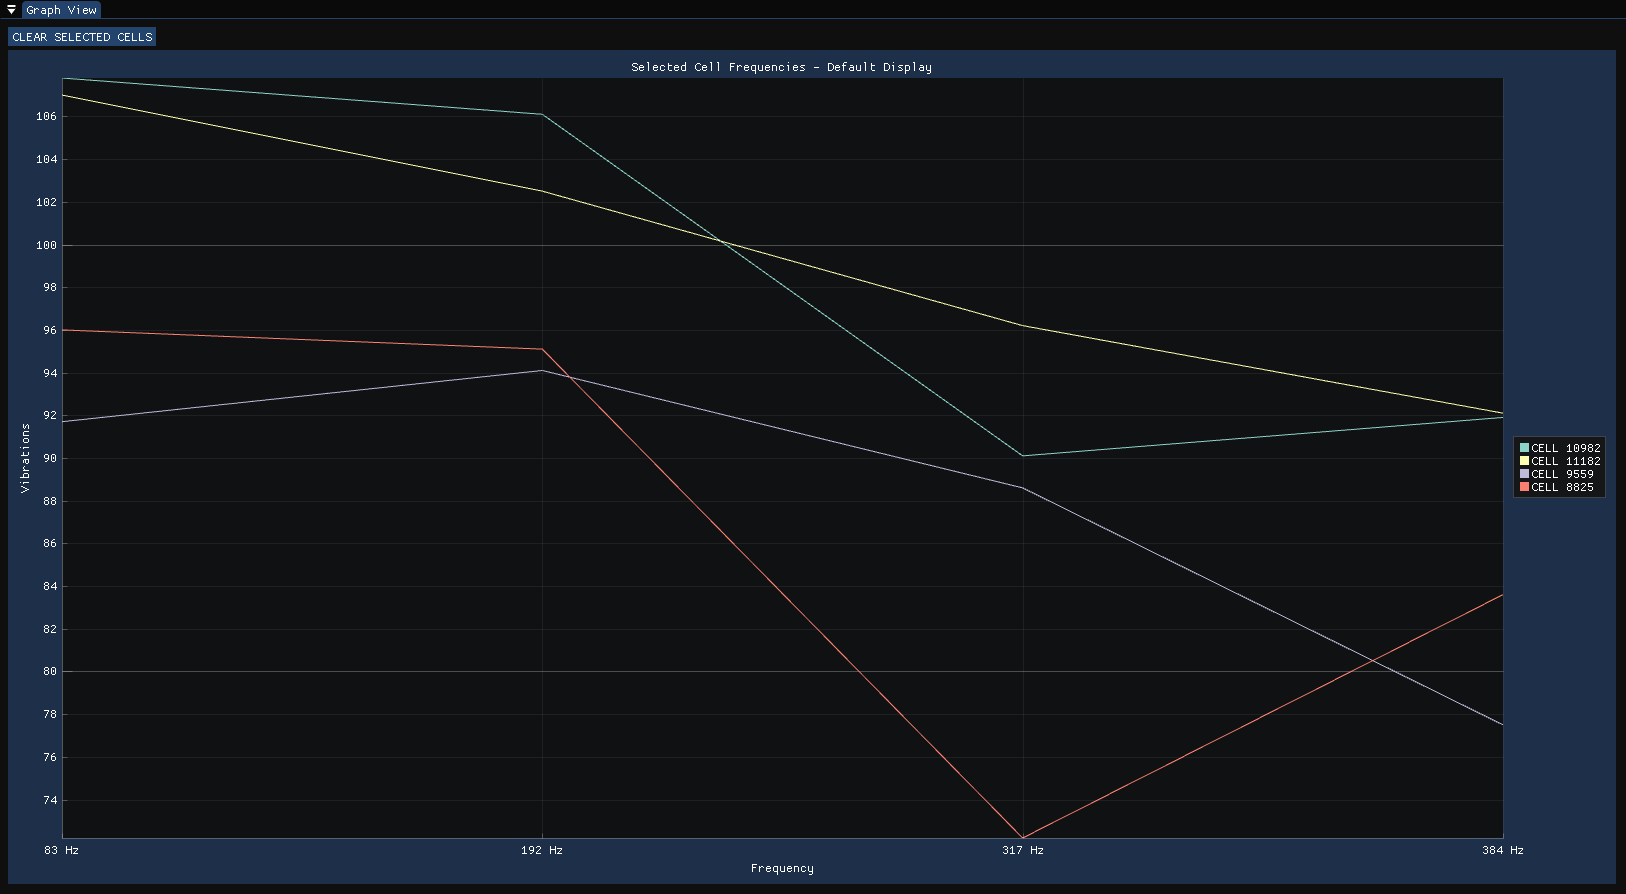
\includegraphics[width=\textwidth]{default_graph_display_lines.png}
	\caption{Normalni način usporedbe grafova u obliku linija}
    \label{appendix:default_graph_display_lines}
\end{figure}

\begin{figure}[H]
	\centering
	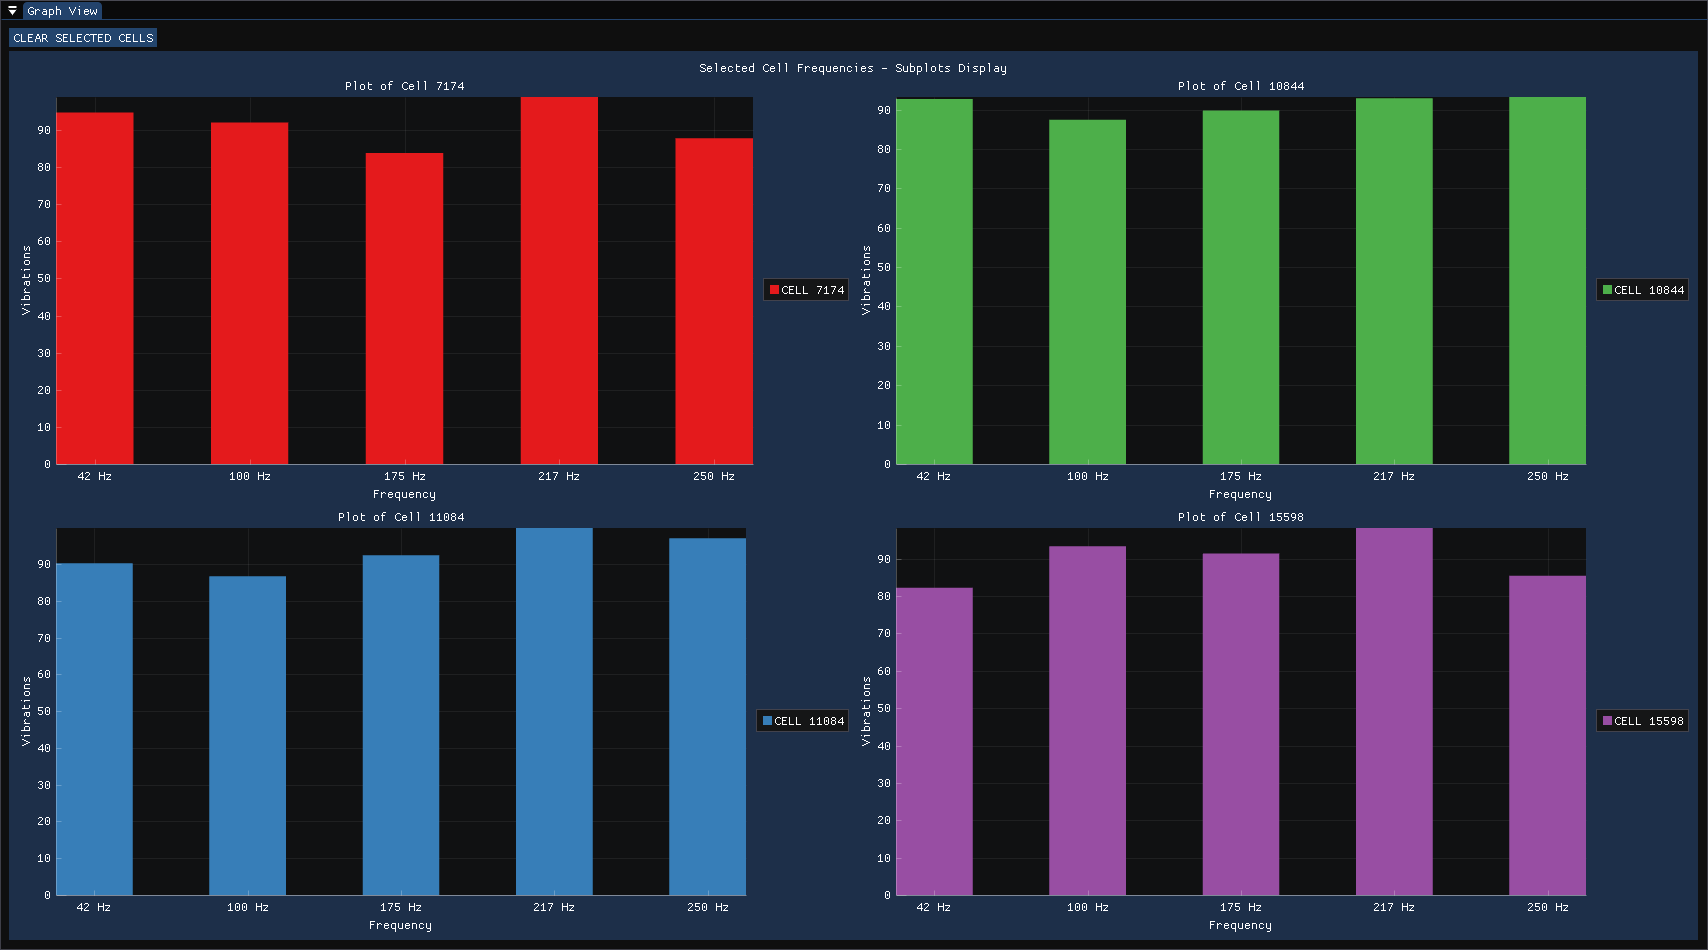
\includegraphics[width=\textwidth]{subplots_graph_display_bars.png}
	\caption{Način usporedbe grafova s višestrukim prikazima u obliku stupaca}
    \label{appendix:subplots_graph_display_bars}
\end{figure}

\begin{figure}[H]
	\centering
	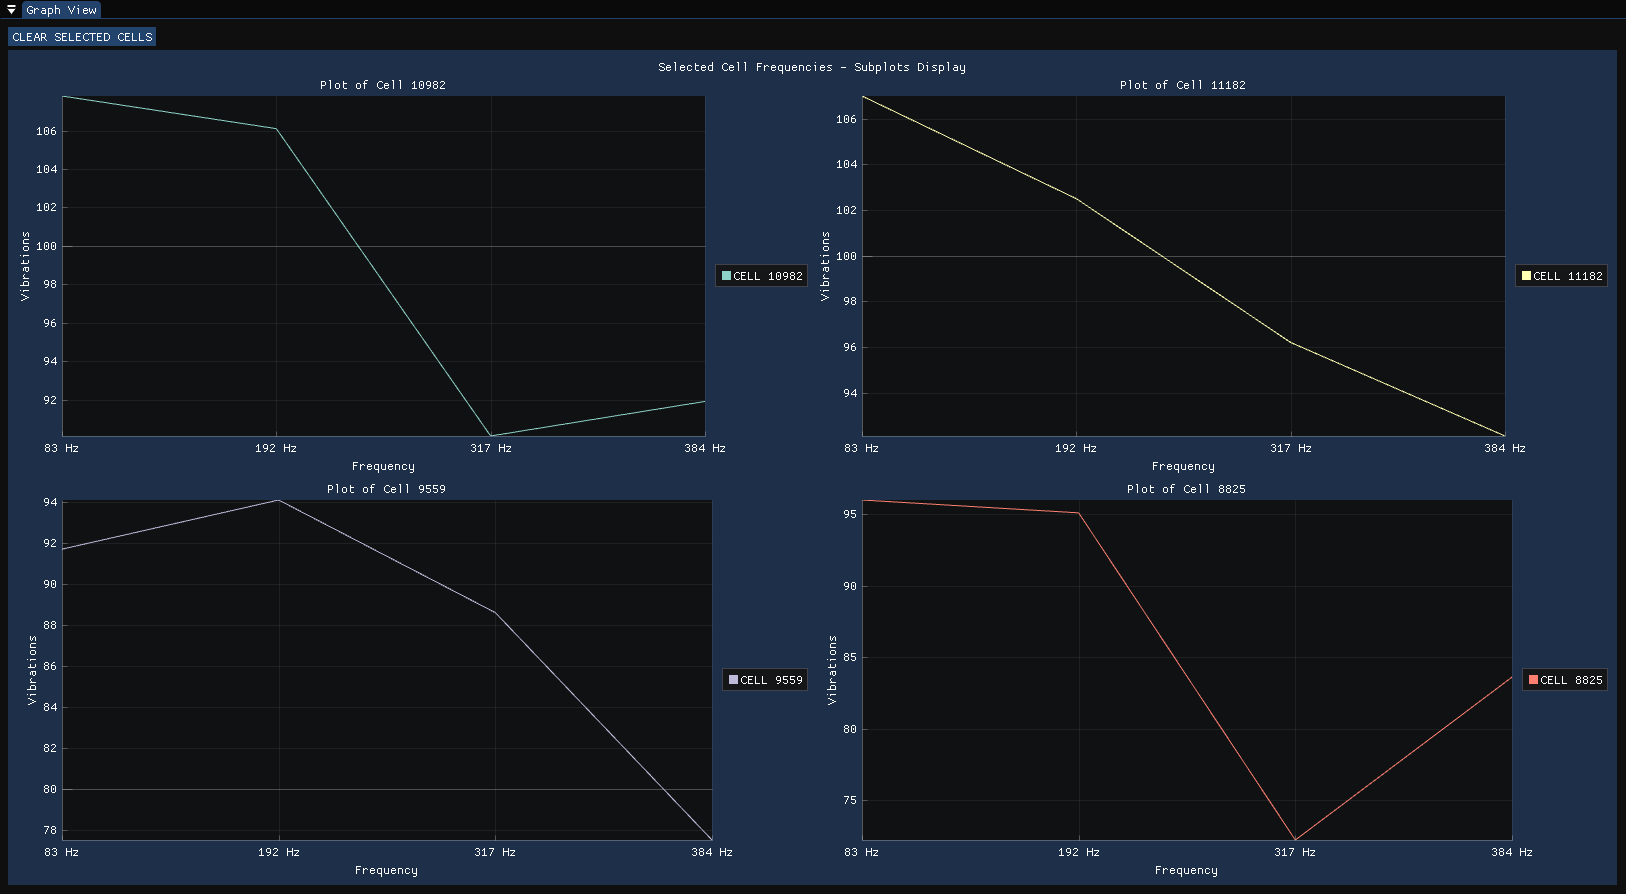
\includegraphics[width=\textwidth]{subplots_graph_display_lines.png}
	\caption{Način usporedbe grafova s višestrukim prikazima u obliku linija}
    \label{appendix:subplots_graph_display_lines}
\end{figure}

\begin{figure}[H]
	\centering
	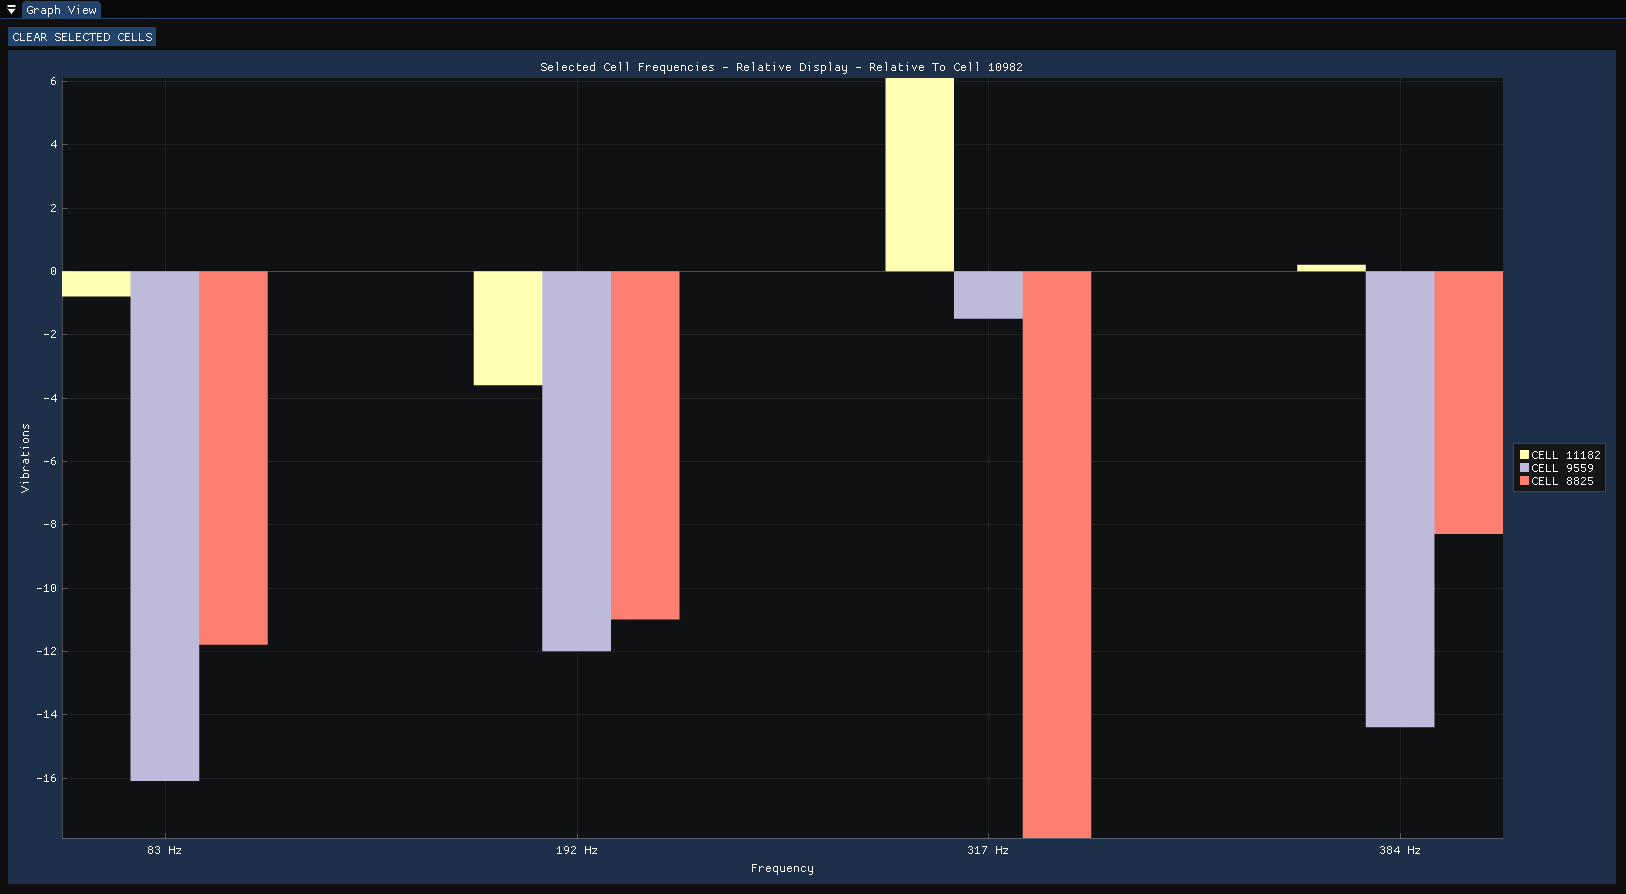
\includegraphics[width=\textwidth]{relative_graph_display_bars_cell_10982.png}
	\caption{Relativni način usporedbe grafova u obliku stupaca u kojem su podaci svih ćelija prikazani u odnosu na ćeliju 10982}
    \label{appendix:relative_graph_display_bars}
\end{figure}

\begin{figure}[H]
	\centering
	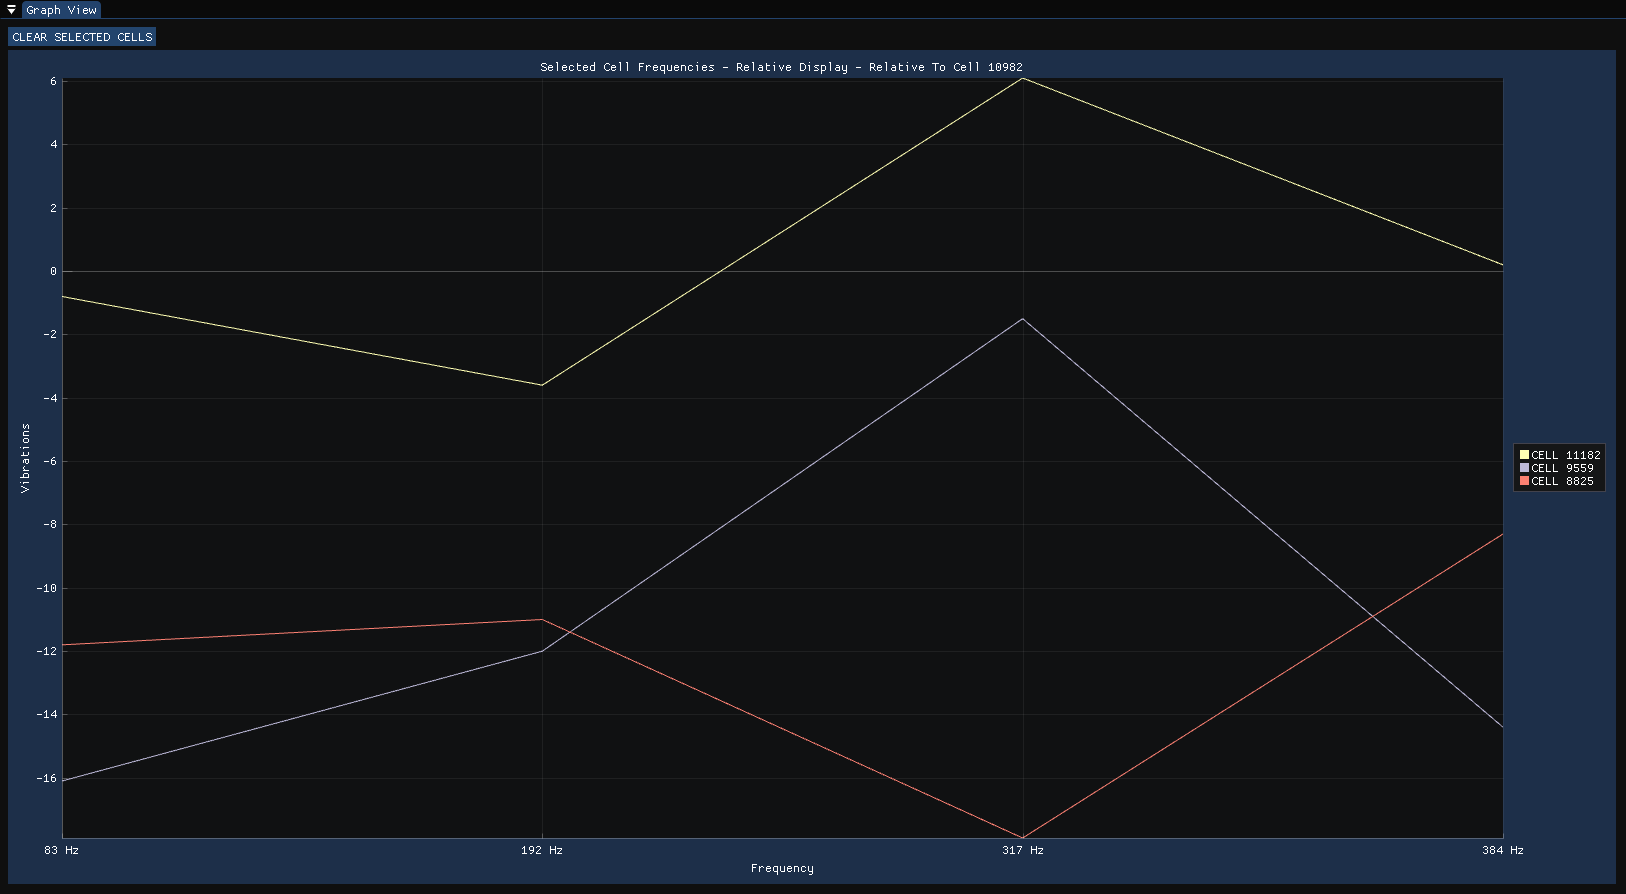
\includegraphics[width=\textwidth]{relative_graph_display_lines_cell_10982.png}
	\caption{Relativni način usporedbe grafova u obliku linija u kojem su podaci svih ćelija prikazani u odnosu na ćeliju 10982}
    \label{appendix:relative_graph_display_lines}
\end{figure}

\chapter{Sustav događaja i signala} \label{appendix:event-signal-system}

Sustav događaja i signala je razvijen u sklopu ovog rada kako bi se olakšalo korištenje obrasca Promatrač. Sustav je implementiran pomoću klasa \textit{Event} i  \textit{Signal} čiji je k\^{o}d prikazan u nastavku.\\

\begin{lstlisting}[caption={Klasa \textit{Event}},captionpos=b]
template <typename T>
class Event {
private:
	std::vector<std::function<void(T)>> m_listeners;
public:
	void add_listener(std::function<void(T)> listener) {
	 m_listeners.push_back(listener); 
	}
	
	template <typename L>
	void add_member_listener(void(L::*m)(T), L* l) {
	 add_listener(std::bind(m, l, std::placeholders::_1)); 
	}
	
	void invoke(T var) {
	for (auto& l : m_listeners)
		l(var);
	}
};
\end{lstlisting}

\begin{lstlisting}[caption={Klasa \textit{Signal}},captionpos=b]
class Signal {
private:
	std::vector<std::function<void()>> m_listeners;
public:
	void add_listener(std::function<void()> listener) { m_listeners.push_back(listener); }

	template <typename L>
	void add_member_listener(void(L::* m)(), L* l) { add_listener(std::bind(m, l)); }

	void invoke() {
	for (auto& l : m_listeners)
		l();
	}
};
\end{lstlisting}
\
\\

Obje klase funkcioniraju na način da im se u listu "promatrača" doda funkcija koju instanca ovih klasa zatim pozove kada se pozove članska funkcija \textit{invoke}. Kada se pozove spomenuta funkcija nad objektom klase \textit{Event}, funkciji je potrebno predati argument koji će ona proslijediti svim funkcijama koje su "pretplaćene" na taj događaj. S druge strane, funkcija \textit{invoke} klase \textit{Signal} ne prima argumente jer sve funkcije koje se "pretplaćuju" na instance ove klase također ne primaju argumente.\\

U obje navedene klase postoje dvije različite funkcije koje služe za registriranje funkcija koje se pozivaju pri aktivaciji događaja: \textit{add\_listener} i \textit{add\_member\_listener}. Funkcija \textit{add\_member\_listener} služi za "registriranje" članskih funkcija jer one zahtijevaju dodatno definiranje pokazivača na objekt čiju se člansku funkciju poziva. Funkcija \textit{add\_listener} se koristi za dodavanje svih ostalih funkcija.

\begin{sazetak}
Osiguravanje minimalne razine buke motora je jedan od ključnih zadataka inženjera pri projektiranju motora, stoga im je iznimno važno održati vibriranje motora prilikom rada na što nižoj razini jer vibracija motora izravno utječe na buku koju motor proizvodi. NVH \engl{Noise, Vibration, Harshness} simulacije pružaju jednostavan način provjere snage vibracija pojedinih dijelova motora u fazi projektiranja. No, računske simulacije ove vrste nerijetko proizvode podatke koje se ne može jednostavno analizirati, pa alati za vizualizaciju uvelike pomažu stručnjacima kod stvaranja ispravne predodžbe o izračunatim podacima. Ovaj rad opisuje izradu alata za vizualizaciju podataka dobivenih iz NVH simulacije pomoću 3D modela motora i 2D grafova. Fokus predstavljenog alata je omogućavanje jednostavnijeg načina uspoređivanja utjecaja različitih frekvencija vibriranja motora na snagu vibracije motora.

\kljucnerijeci{vizualizacija, 3D, NVH podaci, C++, OpenGL}
\end{sazetak}

\engtitle{3D Interactive Visualization of Vibration Simulation}
\begin{abstract}

Minimizing engine noise presents an important task when designing an engine, so it is of utmost importance to keep the engine vibration strength at the lowest possible level since it directly affects the noise level produced by the engine. NVH (Noise, Vibration, Harshness) simulations provide an easy way to check the vibration strength of individual engine parts at the design stage. However, computational simulations of this kind often produce data that is hard to analyze, so visualization tools help significantly by presenting the calculated data intuitively and understandably. This thesis describes the development of an application for visualizing data obtained from NVH simulation using a 3D engine model and 2D graphs. The focus of the presented tool is to provide a straightforward way to compare the influence of different frequencies of engine vibration on the strength of engine vibration.

\keywords{visualization, 3D, NVH data, C++, OpenGL}
\end{abstract}

\end{document}
